\documentclass[a4paper,oneside,11pt]{memoir}
\AddToHook{cmd/section/before}{\clearpage}
\usepackage[utf8]{inputenc}
\usepackage[T1]{fontenc}
\usepackage{microtype}
\usepackage[dvips]{graphicx}
\usepackage{xcolor}
\usepackage{bookman}
\usepackage{graphicx,xcolor}
\usepackage[usestackEOL]{stackengine}
\usepackage[percent]{overpic}
\usepackage{amssymb}
\usepackage{xcolor,framed,marginnote,blindtext}
\usepackage[british]{babel}
\usepackage{longtable}
\usepackage{pdflscape}
\usepackage{makecell}
\usepackage{colortbl}
\usepackage{array}
\usepackage{csquotes}
\usepackage{nicematrix,tikz}
\usepackage{stix}
\usepackage{xcolor}

\usepackage{tabularray}

\usepackage[useregional]{datetime2}

\usepackage{xstring}

\usepackage{topskycolors}

\usepackage{enumitem}

\usepackage[export]{adjustbox}

\usepackage{utfsym}

\usepackage{multirow}

\usepackage{float}

\usepackage{sidecap}

\usepackage{graphicx,capt-of}

\usepackage{biblatex}
\addbibresource{refs.bib}

\usepackage{geometry}

\usepackage{microtype}

\usepackage{cellspace}
\setlength\cellspacetoplimit{4pt}
\setlength\cellspacebottomlimit{4pt}

\usepackage[scaled]{helvet}

\renewcommand\familydefault{\sfdefault} 

\renewcommand*{\arraystretch}{1.6}

\newcounter{rowcounter}

\newcommand{\nextrow}{\refstepcounter{rowcounter}}

\newcommand{\rev}{Rev.1}

\newcommand{\colorref}[1]{\colorbox{Flight Highlight}{\color{#1}#1}}

\newcommand{\colortabex}[1]{\cellcolor{Flight Highlight}\color{#1}\colorref{#1}}

\newcommand{\colortab}[1]{\cellcolor{Flight Highlight}\color{#1}}

\newcommand{\tagref}[1]{\textit{\hyperref[#1]{\StrDel{#1}{tag:}}}}

\newcommand{\stateref}[1]{\textit{\hyperref[state:#1]{#1}}}

\newcommand{\winref}[1]{\textit{\titleref{#1}}}

\newcommand{\image}[1]{\includegraphics[max height=10cm,max width=\textwidth]{#1}}

\newcommand{\drawtag}[3]{\node[draw,red,minimum height=0.55cm,minimum width=#1] at (#2) (#3) {}}

\newcommand{\drawtagdesc}[4]{\node[draw,black,thick,text width=#1] at (#2) (#3) {#4};}

\newcolumntype{P}[1]{>{\centering\arraybackslash}p{#1}}

\newcommand{\headerformat}{%
  {%
 \begin{tabular}{|P{0.1916\textwidth}|P{0.6666\textwidth}|P{0.1416\textwidth}|} 
    \hline
    \raisebox{-0.5\height}{
\includegraphics[max height=0.5\headheight,max width=0.15\textwidth]{img/logo.png}} & \textbf{\large{\leftmark}} & \textbf{\large{\thesection}}  \\
    \scriptsize{TOPLIS User Manual}             & \rightmark         & \small{P\thepage}\         \\
    \hline
    \end{tabular}%
}%
}


\newcommand\capdimage[2]{
\begin{center}
\hspace{1em}%
\vtop{%
\centering
\includegraphics[max height=8cm,max width=8cm]{#1}%
\captionof{figure}{#2}%
}%
\end{center}
\ignorespaces}

\newcolumntype{t}{>{\tt}c}

\colorlet{shadecolor}{gray!20}

\makeatletter
\def\maxwidth#1{\ifdim\Gin@nat@width>#1 #1\else\Gin@nat@width\fi}
\makeatother

\newcommand{\warn}[1]{
  \begin{center}
    
    \begin{tabular}{| P{1.5cm}|p{10.5cm} |}
      \hline
      \cellcolor{shadecolor}\colorbox{red}{\color{white}Warning} &\cellcolor{shadecolor} #1 \\ \hline
    \end{tabular}
  \end{center}
}

\newcommand{\note}[1]{
  \begin{center}
    
    \begin{tabular}{| P{1.5cm}|p{10.5cm} |}
      \hline
      \cellcolor{shadecolor}\colorbox{gray}{\color{white}Note} &\cellcolor{shadecolor} #1 \\ \hline
    \end{tabular}
  \end{center}
}

\DTMlangsetup[en-GB]{abbr,ord=omit,monthyearsep={\space}}

\usepackage[
breaklinks=true,colorlinks=true,
%linkcolor=blue,urlcolor=blue,citecolor=blue,% PDF VIEW
linkcolor=.,urlcolor=black,citecolor=black,% PRINT
bookmarks=true,bookmarksopenlevel=2]{hyperref}

% PDF VIEW
%\geometry{total={210mm,297mm}}
% PRINT
%\geometry{total={210mm,297mm},
%left=20mm,right=20mm,
%bindingoffset=10mm, top=25mm,bottom=25mm}

%PAGE SETUP
\setstocksize{297mm}{210mm}
\settrimmedsize{297mm}{210mm}{*}
\settrims{0pt}{0pt}
\settypeblocksize{230mm}{166mm}{*}
\setlrmargins{*}{34mm}{*}
\setulmargins{42mm}{*}{*}
\setheadfoot{20mm}{15mm}
\setmarginnotes{1mm}{15mm}{1mm}
\checkandfixthelayout

%\OnehalfSpacing
%\linespread{1.3}
\setlength{\parindent}{0pt}

\pretolerance=5000
\tolerance=9000 
\emergencystretch=0pt
\righthyphenmin=4
\lefthyphenmin=4

%%% CHAPTER'S STYLE
\chapterstyle{bianchi}
%\chapterstyle{ger}
%\chapterstyle{madsen}
%\chapterstyle{ell}
%%% STYLE OF SECTIONS, SUBSECTIONS, AND SUBSUBSECTIONS
\setsecheadstyle{\Large\bfseries\sffamily\raggedright}
\setsubsecheadstyle{\large\bfseries\sffamily\raggedright}
\setsubsubsecheadstyle{\bfseries\sffamily\raggedright}

%%% STYLE OF PAGES NUMBERING
%\pagestyle{companion}\nouppercaseheads 
%\pagestyle{headings}
%\pagestyle{Ruled}

\addtopsmarks{plain}{}{ 
  \createmark{chapter}{left}{nonumber}{}{} 
  \createmark{section}{right}{nonumber}{}{} 
} 

\pagestyle{plain}
\makepagestyle{plain}
\makeoddfoot{plain}{\rule{\textwidth}{1pt}\\\today}{}{\rev}
\makeoddhead{plain}{\headerformat}



\maxsecnumdepth{subsubsection} % chapters, sections, and subsections are numbered
\maxtocdepth{subsubsection} % chapters, sections, and subsections are in the Table of Contents

%%%---%%%---%%%---%%%---%%%---%%%---%%%---%%%---%%%---%%%---%%%---%%%---%%%
\begin{document}

%%%---%%%---%%%---%%%---%%%---%%%---%%%---%%%---%%%---%%%---%%%---%%%---%%%
%   TITLEPAGE
%
%   due to variety of titlepage schemes it is probably better to make titlepage manually
%
%%%---%%%---%%%---%%%---%%%---%%%---%%%---%%%---%%%---%%%---%%%---%%%---%%%
\thispagestyle{empty}

{%%%

\centering
\Large

~\vspace{\fill}

{\huge
  \textbf{ 
    \image{img/logo.png}\\
    TOPLIS
}
}

\vspace{2.5cm}

{\LARGE
USER MANUAL
}

\vspace{3.5cm}

TopSky plugin for Portugal vACC

\medskip

Version 2.0

\medskip

\vspace{\fill}

\today

%%%
}%%%

\cleardoublepage
%%%---%%%---%%%---%%%---%%%---%%%---%%%---%%%---%%%---%%%---%%%---%%%---%%%
%%%---%%%---%%%---%%%---%%%---%%%---%%%---%%%---%%%---%%%---%%%---%%%---%%%

\tableofcontents*

\clearpage

%%%---%%%---%%%---%%%---%%%---%%%---%%%---%%%---%%%---%%%---%%%---%%%---%%%
%%%---%%%---%%%---%%%---%%%---%%%---%%%---%%%---%%%---%%%---%%%---%%%---%%%

\chapter{Introduction}

\section{Disclaimer}

Although - as its name suggests - the TopSky plugin is based on TOPLIS and the TopSky ATM system, it is in no way affiliated with or endorsed by Thales Group or NAV Portugal. Similarities between plugin features and the real system are not entirely coincidental, but the plugin can not be used as a real world training aid.

\section{Foreword}

EuroScope, a controller client developed by Gergely Csernák for the VATSIM network, was first released for public use in September 2007. One of the biggest changes in version 3.1 was the possibility for the user community to customize the program to an even higher degree than was possible before by writing their own plugins that can be used to alter the way information is presented and even create completely new functionality into the program. This allowed creating very detailed simulations of all kinds of ATC systems without making the main program overly complex. Version 3.2 expands on these possibilities, making it possible to create even better plugins.

\bigskip

The base TopSky plugin is developed by Juha Holopainen of VATSIM Scandinavia. The TopSky plugin (a.k.a. The Plugin Formerly Known As “EUROCAT 2000 E”) started out as a very small project to create a couple of customized aircraft tag items, but as more information about the real system and the possibilities with the plugin development became available, it slowly grew to include an almost complete set of tag items, tag menus, graphical elements on the radar display and some additional functionality.\cite{topskygen}

\bigskip

The A-CDM plugin is developed by Roger Puig of VatSpa. CDM is an Euroscope plugin based on the real life CDM tool that allows us to improve the departure flows at airports.\cite{cdm}

\chapter{Systems}

\section{A-CDM}

Airport CDM (A-CDM) aims to improve the efficiency and resilience of airport operations by optimising the use of resources and improving the predictability of air traffic. 

It also allows the exchange of more accurate departure information, particularly target take-off times, with the European ATFCM network, leading to improved en-route and sectoral planning.\cite{eurocontrol}

\subsection{Operation}

The A-CDM plugin operates in a Master-Slave topology, in which the "CDM Master" will calculate the required data and distribute it to the slaved CDM positions. Due to this, it is mandatory that the "Master" ATC is the one at the lowest position, such as Delivery.

\warn{IF THERE IS NO ACTIVE "CDM MASTER" A-CDM WILL NOT BE OPERATIONAL}
  


\warn{IF MORE THAN ONE POSITION ASSIGNS ITSELF AS "CDM MASTER" A-CDM WILL NOT BE OPERATIONAL}

At the end of a session or controller swap, the "CDM MASTER" ATC should return himself to "CDM SLAVE" before the next controller takes over.

\subsubsection{A-CDM Timeline}

\begin{figure}
  \centering
  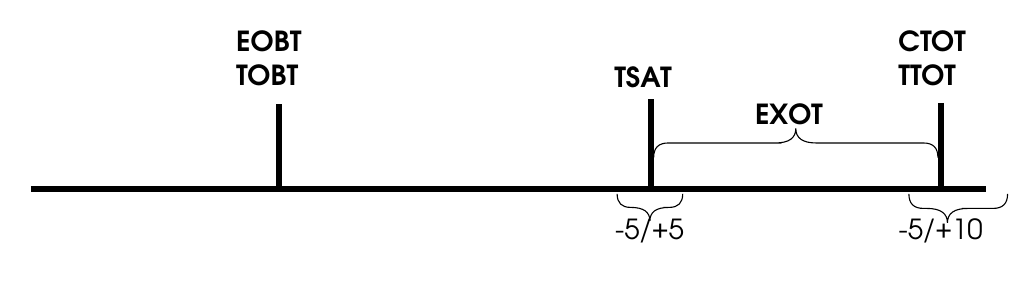
\begin{tikzpicture}[x=0.75pt,y=0.75pt,yscale=-1,xscale=1]
    \path (0,121); 
    
    \draw [line width=2.25]    (0,84.09) -- (\textwidth,84.09) ;
    \draw [line width=2.25]    (438.47,42.6) -- (438.47,84.41) ;
    \draw [line width=2.25]    (298.69,40.97) -- (298.69,82.78) ;
    \draw [line width=2.25]    (119.42,43.39) -- (119.42,85.2) ;
    \draw   (282.5,86.46) .. controls (282.5,90.8) and (284.67,92.97) .. (289,92.97) -- (289,92.97) .. controls (295.19,92.97) and (298.29,95.14) .. (298.29,99.47) .. controls (298.29,95.14) and (301.39,92.97) .. (307.59,92.97)(304.8,92.97) -- (307.59,92.97) .. controls (311.92,92.97) and (314.09,90.8) .. (314.09,86.46) ;
    \draw   (423.07,86.46) .. controls (423.07,91.13) and (425.4,93.46) .. (430.07,93.46) -- (431.63,93.46) .. controls (438.3,93.46) and (441.63,95.79) .. (441.63,100.46) .. controls (441.63,95.79) and (444.96,93.46) .. (451.63,93.46)(448.63,93.46) -- (463.62,93.46) .. controls (468.29,93.46) and (470.62,91.13) .. (470.62,86.46) ;
    \draw   (437.06,68.94) .. controls (437.06,64.27) and (434.73,61.94) .. (430.06,61.94) -- (378.58,61.94) .. controls (371.91,61.94) and (368.58,59.61) .. (368.58,54.94) .. controls (368.58,59.61) and (365.25,61.94) .. (358.58,61.94)(361.58,61.94) -- (307.1,61.94) .. controls (302.43,61.94) and (300.1,64.27) .. (300.1,68.94) ;
    
    \draw (416.76,6.65) node [anchor=north west][inner sep=0.75pt]   [align=left] {\textbf{CTOT}\\\textbf{TTOT}};
    \draw (279.87,23.86) node [anchor=north west][inner sep=0.75pt]   [align=left] {\textbf{TSAT}};
    \draw (97.71,6.65) node [anchor=north west][inner sep=0.75pt]   [align=left] {\textbf{EOBT}\\\textbf{TOBT}};
    \draw (280.29,97.31) node [anchor=north west][inner sep=0.75pt]   [align=left] {\mbox{-}5/+5};
    \draw (416.87,97.31) node [anchor=north west][inner sep=0.75pt]   [align=left] {\mbox{-}5/+10};
    \draw (347.71,41.46) node [anchor=north west][inner sep=0.75pt]   [align=left] {\textbf{EXOT}};
  \end{tikzpicture}
  \caption{A-CDM timeline with delaying TSAT example} \label{fig:acdm}
\end{figure}

Each departure follows a timeline of events from the moment a Flight Plan is submitted until the flight is airborne. These events are called "Milestones".

\medskip

Every Flight Plan should have a meaningfull Estimated Off Block Time (EOBT, also known as ETD). The EOBT is the starting point for the A-CDM calculation from which A-CDM will set the Target Off Block Time (TOBT) equal to. If the ATC notices TOBT is not meaningfull (already in the past or too far into the future) it must be updated.

\medskip

A-CDM will calculate a Target Take Off Time (TTOT) based on the TOBT, current departure rate, known traffic and Flow Restrictions. Each TTOT is separated from other TTOTs by the ammount of time required in order to achieve the maximum defined departure rate. During moments of high traffic that, without a regulation, would exceed the airport departure rate capacity, the system will delay the TTOT in order to meet the required departure rate. 

\medskip

Based on the Departure Stand and Runway, the system calculates an Estimated Taxi Out Time (EXOT). Then, the system subtracts TTOT-EXOT, of which the result is the Target Start-up Time (TSAT). TSAT may never be earlier than TOBT. A TSAT has a validity window of -5 to +5 minutes, within which start-up approval may be issued. 

A TSAT within the validity window will be colored in \colorref{color1}, or if outside the validity window \colorref{color2}. Additionally, it will be colored in \colorref{color5} the minute it expires, as an attention getter.

If a flight misses its TSAT, a new one must be assigned by right clicking the TSAT value in order to set TOBT to present time and restart the CDM calculation for the concerned flight.

\medskip

During times of extraordinary demand, a Calculated Take-Off Time (CTOT) may be issued for a certain flight. The A-CDM operation remains the same, with the exception that it will try to match TTOT to CTOT. A CTOT has a validity window of -5 to +10 minutes of CTOT, during which Take Off clearance must be issued.    

\subsubsection{Commands}

Interaction with core A-CDM systems is done with classic command line inputs:

\begin{longtable}{|p{5cm}|p{8.5cm}|}
  \hline
  \texttt{.cdm reload}                 & Reloads all CDM configs\\ \hline
  \texttt{.cdm refresh}                & Forces a data refresh phase\\ \hline
  \texttt{.cdm save}                   & Saves data to \texttt{savedData.txt}\\ \hline
  \texttt{.cdm load}                   & Loads \texttt{savedData.txt}\\ \hline
  \texttt{.cdm master "airport"}       & Become the master of the selected airport.\\ \hline
  \texttt{.cdm slave "airport"}        & Turn back to slave of the selected airport.\\ \hline
  \texttt{.cdm refreshtime "seconds"}  & Change refresh rate time in seconds (Default 30, MAX 99).\\ \hline
  \texttt{.cdm delay "minutes"}        & Adds delay minutes to all flights that have a TSAT in the future\\ \hline
  \texttt{.cdm lvo}                    & Toggle LVO on or off\\ \hline
  \texttt{.cdm realmode}               & Toggle realmode on or off\\ \hline
  \texttt{.cdm remarks}                & Toggle set TSAT to Euroscope scratchpad on or off\\ \hline
  \texttt{.cdm rates}                  & Updates rates values from \texttt{rate.txt}\\ \hline
  \texttt{.cdm help}                   & Show all commands \\ \hline
  \caption{A-CDM commands}
  \label{tab:acdm-commands}
\end{longtable}



\subsection{A-CDM field descriptions}

\begin{longtable}{|p{2.5cm}|p{2.5cm}|p{4.5cm}|p{4.5cm}|}
  \hline
  \textbf{Data field}             &  \textbf{Description}     &  \textbf{Comments}                    &  \textbf{Color} \\ \hline  \endhead
  A \nextrow \label{tag:CDM A}&  
    Alert & 
      Flashes A if the aircraft is waiting for an action&
        \colorref{color5}\\ \hline

  ASAT \nextrow \label{tag:ASAT}&  
    Actual Start-Up Approval Time &
        Automatically records time of Start-Up Approval when inputting a Start-Up, Pushback, Taxi or DEPA Ground Status &   
          \colorref{color12} \\ \hline

  ASRT \nextrow \label{tag:ASRT}&  
    Actual Start-Up Request Time &
        Used to record time of Ready or Start-Up Request &   
          \colorref{color10} \\ \hline
  
  CTOT \nextrow \label{tag:CTOT}&  
      Calculated Take Off Time&
        Flow restrictions create CTOTs to planes afected with published MDIs from ECFMP &   
            \colorref{color11} \\ \hline

  E \nextrow \label{tag:E}&  
    State & 
      Depending on aircraft timming:

      P: EOBT more than 35 minutes in the future

      C: EOBT is less than 35min and TSAT not expired

      I: TSAT expired &
        \\ \hline            

            
  EOBT \nextrow \label{tag:EOBT}&  
    Estimated Off Block Time & 
      Same time as Flight Plan ETD or EOBT &
        \colorref{color8} 

        \bigskip

        If a new EOBT is submitted by the pilot, and EOBT is different than TOBT:

        \colorref{color4} \\ \hline

  
  Flow Message \nextrow \label{tag:Flow Message}&  
    ECFMP Flow Message&
        Description of the restriction impacting the flight &   
          \colorref{color8}\\ \hline

  Ready \nextrow \label{tag:Ready}&  
    Ready State Flag&
      Used to signal Ready state. Setting Ready also records time of Ready or Start-Up Request &   
        Ready:
        
        \colorref{color1} 
        
        \bigskip
        
        Not Ready:
        
        \colorref{color7}\\ \hline
      
  TOBT \nextrow \label{tag:TOBT}&  
    Target Off Block Time & 
      On receipt of a new Flight Plan, TOBT is set to the same time as EOBT. 

      \bigskip

      If the Flight Plan is updated with a new EOBT, TOBT will not change automatically. 

      If required, TOBT may be manually updated using the Edit TOBT function &
        From TOBT-35 to TOBT-5

        \colorref{color2} 

        \bigskip

        From TOBT-5 to TOBT+5:

        \colorref{color1} \\ \hline

  TSAC \nextrow \label{tag:TSAC}&  
    Target Start-Up Approval Communicated Time&
      Used to note down TSAT communicated to the flight&   
       If TSAC within 5 minutes of TSAT:

       \colorref{color1}

       If TSAT changed by more than 5 minutes:

       \colorref{color4} \\ \hline

  TSAT \nextrow \label{tag:TSAT}&  
    Target Startup Time & 
      TTOT - EXOT &   
        From EOBT-35 to TSAT-5:
        
        \colorref{color2}

        \bigskip

        From TSAT-5 to TSAT+5:

        \colorref{color1}

        \bigskip

        From TSAT+5 to TSAT+6:

        \colorref{color5}

        \bigskip

        After TSAT+6:
        
        \colorref{color2}\\ \hline

  TTOT \nextrow \label{tag:TTOT}&  
    Target Take Off Time &
      &   
        \colorref{color9}\\ \hline
        \caption{A-CDM field descriptions}
        \label{tab:acdm-items}
\end{longtable}

\section{Coordination}

TopSky provides various ways to coordinate information between controllers.

\bigskip

The example track labels do not represent any specific setup and are only meant to highlight the items specific to each function. In the examples, aircraft ABC123 is assumed by “transferring controller” and the next sector is referred to as “accepting controller”. For reference, the example labels would look like these before any coordination (coordination point TROIA, entry/exit level FL180):

\bigskip

\begin{longtable}{p{0.45\textwidth} p{0.45\textwidth}}
  Transferring controller:

  \begin{tabular}{
    >{\columncolor{Flight Highlight}}l 
    >{\columncolor{Flight Highlight}}l
    >{\columncolor{Flight Highlight}}l }
    {\color{Assumed} ABC123} & {\color{Coordination} IDA}       & {\color{Assumed} }      \\
    {\color{Assumed} 100}    & {\color{Assumed} $\blacktriangle$} & {\color{Assumed} TROIA} \\
    {\color{Assumed} 180}    & {\color{Assumed} }          & {\color{Assumed} }     
  \end{tabular}
  &

  Accepting controller:

  \begin{tabular}{
    >{\columncolor{Flight Highlight}}l 
    >{\columncolor{Flight Highlight}}l
    >{\columncolor{Flight Highlight}}l }
    {\color{Coordination} ABC123} & {\color{Coordination} IDT}       & {\color{Coordination} }      \\
    {\color{Coordination} 100}    & {\color{Coordination} $\blacktriangle$} & {\color{Coordination} TROIA} \\
    {\color{Coordination} 180}    & {\color{Coordination} }          & {\color{Coordination} }     
  \end{tabular}
  \end{longtable}

\bigskip

Some of the coordination functions (ROF, RTI and TIP) require very specific conditions to exist to be able to send the necessary messages between the controllers. TopSky attempts to check for this and either disables the function (grey text in the menu button) or creates a warning message if the conditions are lost during a coordination, but in some cases the coordination messages can get lost. In this case try the coordination again or manually coordinate.

\subsection{PEL/COPN}

A coordination is displayed by coloring the proposed values \colorref{Proposition In} or \colorref{Proposition Out}, depending on whether the coordination was sent or received, in the track label and the flight lists. Additionally, a message is displayed in the \winref{win:miw} for received coordinations and in the \winref{win:mow} for coordinations sent by you.

\bigskip

To send a PEL (Planned Entry Level) coordination, left-click on the PEL value in the track label or a flight list. This opens a menu to select a value. To send a COPN (Entry Point) coordination, left-click on the COPN value in the track label or a flight list. This opens the \winref{menu:wpt}. Select “Routing”. This opens a menu to select the desired point. The response of the coordination can be a counter-proposal as well, in which case the color of the values remain \colorref{Proposition In}.

\bigskip

An example track label, showing both the PEL and COPN being coordinated:

\bigskip

\begin{tabular}{
  >{\columncolor{Flight Highlight}}l 
  >{\columncolor{Flight Highlight}}l
  >{\columncolor{Flight Highlight}}l }
  {\color{Coordination} ABC123} & {\color{Coordination} IDT}       & {\color{Coordination} }      \\
  {\color{Coordination} 100}    & {\color{Coordination} $\blacktriangle$} & {\color[RGB]{225,130,180} TROIA} \\
  {\color[RGB]{225,130,180} 180}    & {\color{Coordination} }          & {\color{Coordination} }     
\end{tabular}

\bigskip

To answer an incoming coordination, left-click on a proposed value or the corresponding message in the \winref{win:miw}. This opens a menu where you can select the response (Accept, Refuse or Change). After the response, the track label and lists display depend on the answer:

\bigskip

\begin{tabular}{l l}
  Accept: & Accepted values, sector state color\\
  Refuse: & Original values, sector state color (due to EuroScope bug, should be \colorref{Warning})\\
  Change: & New proposed values in \colorref{Proposition Out}\\
\end{tabular}

\subsection{XFL/COPX}

A coordination is displayed by coloring the proposed values \colorref{Proposition In} or \colorref{Proposition Out}, depending on whether the coordination was sent or received, in the track label and the flight lists. Additionally, a message is displayed in the \winref{win:miw} for received coordinations and in the \winref{win:mow} for coordinations sent by you.

\bigskip

To send an XFL (Exit Flight Level) coordination, left-click on the XFL value in the track label or a flight list. This opens a menu to select a value. To send a COPX (Exit Point) coordination, left-click on the COPX value in the track label or a flight list. This opens the \winref{menu:wpt}. Select “Routing”. This opens a menu to select the desired point. The response of the coordination can be a counter-proposal as well, in which case the color of the values remain \colorref{Proposition In}.

\bigskip

An example track label, showing both the XFL and COPX being coordinated:

\bigskip

\begin{tabular}{
  >{\columncolor{Flight Highlight}}l 
  >{\columncolor{Flight Highlight}}l
  >{\columncolor{Flight Highlight}}l }
  {\color{Assumed} ABC123} & {\color{Coordination} IDA}       & {\color{Assumed} }      \\
  {\color{Assumed} 100}    & {\color{Assumed} $\blacktriangle$} & {\color[RGB]{225,130,180} TROIA} \\
  {\color{Assumed} 180}    & {\color[RGB]{225,130,180} 200}          & {\color{Assumed} }     
\end{tabular}

\bigskip

To answer an incoming coordination, left-click on a proposed value or the corresponding message in the \winref{win:miw}. This opens a menu where you can select the response (Accept, Refuse or Change). After the response, the track label and lists display depend on the answer:

\bigskip

\begin{tabular}{l l}
  Accept: & Accepted values, sector state color\\
  Refuse: & Original values, sector state color (due to EuroScope bug, should be \colorref{Warning})\\
  Change: & New proposed values in \colorref{Proposition Out}\\
\end{tabular}

\subsection{Releases}

To communicate a release to the next controller, select the “Trf \& release” option instead of “Transfer” in the \winref{menu:cs} when transferring the aircraft. This opens the \winref{menu:xfrrel} to select the desired release condition. The available choices are “Climb”, “Descent”, “Turn” and “Full”. Selecting an option will start the transfer with the selected release condition.

\bigskip

The release will be displayed on line 0 of the track label (in \colorref{Proposition In} or \colorref{Proposition Out} during the transfer), showing the first letter of the release condition. The example labels below show a Full release:

\bigskip

\begin{longtable}{p{0.45\textwidth} p{0.45\textwidth}}
  Transferring controller:

\begin{tabular}{
  >{\columncolor{Flight Highlight}}l 
  >{\columncolor{Flight Highlight}}l
  >{\columncolor{Flight Highlight}}l }
  {\color{Proposition In} F} & {\color{Coordination} }       & {\color{Assumed} }      \\
  {\color{Proposition In} ABC123} & {\color{Proposition In} IDA}       & {\color{Assumed} }      \\
  {\color{Assumed} 100}    & {\color{Assumed} $\blacktriangle$} & {\color{Assumed} TROIA} \\
  {\color{Assumed} 180}    & {\color{Assumed} }          & {\color{Assumed} }     
\end{tabular}
&

  Accepting controller:

\begin{tabular}{
  >{\columncolor{Flight Highlight}}l 
  >{\columncolor{Flight Highlight}}l
  >{\columncolor{Flight Highlight}}l }
  {\color{Proposition In} F} & {\color{Coordination} }       & {\color{Assumed} }      \\
  {\color{Assumed} ABC123} & {\color{Assumed} IDT}       & {\color{Coordination} }      \\
  {\color{Coordination} 100}    & {\color{Coordination} $\blacktriangle$} & {\color{Coordination} TROIA} \\
  {\color{Coordination} 180}    & {\color{Coordination} }          & {\color{Coordination} }     
\end{tabular}
\end{longtable}

\bigskip

After the accepting controller assumes the aircraft, the release indicator changes to sector state color. It remains in the transferring controller’s label until it becomes \stateref{Unconcerned}, and in the accepting controller’s label for 3 minutes.

\note{If a release is sent to a controller not using the TopSky plugin, it will only be displayed on your label. To the accepting controller it will look like a normal transfer.}

\subsection{HOP}
\label{coo:hop}
The purpose of the HOP (Hand-Over Proposal) message is for the transferring controller to propose the flight for hand-over to the accepting controller, and/or to propose non-standard transfer conditions which require the approval of the accepting controller.

\bigskip

To send a HOP without any transfer conditions, select the \winref{win:hop} option in the \winref{menu:cs}.

\bigskip

To send a HOP with a transfer condition (assigned heading, direct-to point or assigned speed):

\begin{enumerate}
  \item open the AHDG or ASP menu and select the "HOP" option (found in the “More” folder)
  \begin{itemize}
    \item See \winref{win:hop} for indications
  \end{itemize}
  \item select the desired value (to select a direct-to point, select the “Point” option in the AHDG menu and then left-click on the point on the radar screen
\end{enumerate}

The example labels below show a HOP with an assigned heading proposal:

\begin{longtable}{p{0.45\textwidth} p{0.45\textwidth}}
  Transferring controller:

\begin{itemize}
  \item SI item and any proposed values in \colorref{Proposition Out} color
  \item Message in Message Out Window
\end{itemize}

\begin{tabular}{
  >{\columncolor{Flight Highlight}}l 
  >{\columncolor{Flight Highlight}}l
  >{\columncolor{Flight Highlight}}l }
  {\color{Assumed} ABC123} & {\color{Proposition In} IDA}       & {\color{Assumed} }\\
  {\color{Assumed} 100}    & {\color{Assumed} $\blacktriangle$} & {\color{Assumed} TROIA}\\
  {\color{Assumed} 180}    & {\color{Assumed} }          & {\color{Assumed} }\\  
  {\color{Proposition In} H360}    & {\color{Assumed} }          & {\color{Assumed} }\\  
\end{tabular}
  &
  
  Accepting controller:

\begin{itemize}
  \item Callsign item and any proposed values in \colorref{Proposition In} color
  \item Message in Message In Window
\end{itemize}

\begin{tabular}{
  >{\columncolor{Flight Highlight}}l 
  >{\columncolor{Flight Highlight}}l
  >{\columncolor{Flight Highlight}}l }
  {\color{Proposition In} ABC123} & {\color{Coordination} IDT}       & {\color{Coordination} }\\
  {\color{Coordination} 100}    & {\color{Coordination} $\blacktriangle$} & {\color{Coordination} TROIA}\\
  {\color{Coordination} 180}    & {\color{Coordination} }          & {\color{Coordination} }\\
  {\color{Proposition In} H360}    & {\color{Coordination} }          & {\color{Coordination} }\\      
\end{tabular}
\end{longtable}

\bigskip

The transferring controller should monitor both the track label and the \winref{win:miw} as there are three ways for the accepting controller to answer a HOP. In order of preference, they are:

\begin{itemize}
  \item From the \winref{menu:cs}, select “ROF”. This sends a ROF message to the transferring controller.
  \begin{itemize}
    \item See \winref{menu:rof} for indications
  \end{itemize}
  \item Left-click on the AHDG, ASP or COPN item. This opens the \winref{menu:ctm}. In it, select “Accept”. This sends an Accept message to the transferring controller.
  \begin{itemize}
    \item The labels on both controllers’ screens return to normal sector state coloring
    \item A message is put into the Message In Window for the transferring controller
    \item A message is put into the Message Out Window for the accepting controller
  \end{itemize}
  \item From the \winref{menu:cs}, select “Assume”. This assumes the aircraft (with the other two answers the aircraft remains assumed by the transferring controller)
  \begin{itemize}
    \item The labels on both controllers’ screens return to normal sector state coloring
  \end{itemize}
\end{itemize}

\note{If a HOP is sent to a controller not using the TopSky plugin, it will only be displayed on your label. To the accepting controller it will look like a normal transfer. Any proposed values will be shown also on the accepting controller’s label but they will not be colored as proposals.

  If a HOP is sent to a manually selected controller and is answered by either “Accept” or “ROF”, the next controller is reset to the automatically calculated one. The correct controller needs to be manually selected again before transferring the aircraft.}

\subsection{ROF}
\label{coo:rof}

The ROF (Request on Frequency) message is sent by the accepting controller to the transferring controller when a flight establises radio contact but the label has not yet been transfered to the downstream sector. The upstream sector should then transfer the label. The message may also be used as a reply to HOP to signify the acceptance of the flight under the proposed conditions.

\warn{ROF should not be used to request an early handover of a flight. ROF is a coordination tool that is context dependent, using it outside the prescribed scenarios or ir other unintended ways will cause unnecessary confusion.}

To send a ROF message, select the “ROF” option in the \winref{menu:cs} of the aircraft in question. The example label below shows the indications when the message is sent (there are no indications in the accepting controller’s track label):


\begin{longtable}{p{0.45\textwidth} p{0.45\textwidth}}
  Transferring controller:

  \begin{itemize}
    \item ROF text in \colorref{Proposition In} color
    \item Message in Message In Window
  \end{itemize}

  \begin{tabular}{
    >{\columncolor{Flight Highlight}}l 
    >{\columncolor{Flight Highlight}}l
    >{\columncolor{Flight Highlight}}l }
    {\color{Proposition In} ROF} & {\color{Coordination} }       & {\color{Assumed} }      \\
    {\color{Assumed} ABC123} & {\color{Coordination} IDA}       & {\color{Assumed} }      \\
    {\color{Assumed} 100}    & {\color{Assumed} $\blacktriangle$} & {\color{Assumed} TROIA} \\
    {\color{Assumed} 180}    & {\color{Assumed} }          & {\color{Assumed} }     
  \end{tabular}
  &
  
  Accepting controller:

  \begin{itemize}
    \item ROF text in \colorref{Proposition Out} color
    \item Message in Message Out Window
  \end{itemize}
\end{longtable}





















The indications are removed when a “Transfer”, “Trf \& release” or “HOP” is performed.

\note{If a ROF is sent to a controller not using the TopSky plugin or the message fails to go through, an error message will be put into the Personal Queue Window. The message counter in the Global Menu will be highlighted in \colorref{Warning} color if the window is not open.}

\subsection{RTI/TIP}
\label{coo:rti}\label{coo:tip}
These messages are used to request/propose the transfer of a flight on an assigned heading, speed or rate of climb/descent. RTI (Request Tactical Instructions) is a request initiated by the accepting controller and TIP (Tactical Instructions Proposal) a proposal initiated by the transferring controller.

\bigskip

In the examples below the RTI message is used. For the TIP message, the indications and actions are the same, only the roles are reversed – the transferring controller sends and the accepting controller answers the message, so the message will appear in the other Message Window.

To send the RTI message:

\begin{enumerate}
  \item open the AHDG, ASP or ARC menu and select the “RTI” option (found in the “More” folder) 
  \item select the desired value in the list (“Point” option in the AHDG menu is not available)
\end{enumerate}

When the message is sent, the following indications are shown:

\begin{longtable}{p{0.45\textwidth} p{0.45\textwidth}}
  Transferring controller:

  \begin{itemize}
    \item Proposed value in \colorref{Proposition In} color
    \item Message in Message In Window
  \end{itemize}

  \begin{tabular}{
    >{\columncolor{Flight Highlight}}l 
    >{\columncolor{Flight Highlight}}l
    >{\columncolor{Flight Highlight}}l }
    {\color{Proposition In} H360} & {\color{Assumed} }       & {\color{Assumed} }      \\
    {\color{Assumed} ABC123} & {\color{Coordination} IDA}       & {\color{Assumed} }      \\
    {\color{Assumed} 100}    & {\color{Assumed} $\blacktriangle$} & {\color{Assumed} TROIA} \\
    {\color{Assumed} 180}    & {\color{Assumed} }          & {\color{Assumed} }     
  \end{tabular}

  &
 
  Accepting controller:

  \begin{itemize}
    \item Proposed value in \colorref{Proposition Out} color
    \item Message in Message Out Window
  \end{itemize}

  \begin{tabular}{
    >{\columncolor{Flight Highlight}}l 
    >{\columncolor{Flight Highlight}}l
    >{\columncolor{Flight Highlight}}l }
    {\color{Proposition Out} H360} & {\color{Coordination} }       & {\color{Coordination} }      \\
    {\color{Coordination} ABC123} & {\color{Coordination} IDT}       & {\color{Coordination} }      \\
    {\color{Coordination} 100}    & {\color{Coordination} $\blacktriangle$} & {\color{Coordination} TROIA} \\
    {\color{Coordination} 180}    & {\color{Coordination} }          & {\color{Coordination} }     
  \end{tabular}
\end{longtable}

\bigskip

To answer the message, left-click on the proposed value on line 0. This opens the \winref{menu:ttm}) where you can either accept or reject the proposal. When clicking on “Accept”, the menu closes and the following indications are displayed:

\begin{longtable}{p{0.45\textwidth} p{0.45\textwidth}}
  Transferring controller:

  \begin{itemize}
    \item Accepted value in sector state color
    \item Relevant label field value in \colorref{Information} color (until the accepted value is set)
    \item Message in Message Out Window
  \end{itemize}
  
  \begin{tabular}{
    >{\columncolor{Flight Highlight}}l 
    >{\columncolor{Flight Highlight}}l
    >{\columncolor{Flight Highlight}}l }
    {\color{Assumed} H360} & {\color{Assumed} }       & {\color{Assumed} }      \\
    {\color{Assumed} ABC123} & {\color{Coordination} IDA}       & {\color{Assumed} }      \\
    {\color{Assumed} 100}    & {\color{Assumed} $\blacktriangle$} & {\color{Assumed} TROIA} \\
    {\color{Assumed} 180}    & {\color{Assumed} }          & {\color{Assumed} }\\     
    {\color{Information} AHDG}    & {\color{Assumed} }          & {\color{Assumed} }     
  \end{tabular}

  &

  Accepting controller:

  \begin{itemize}
    \item Accepted value in sector state color
    \item Relevant label field value in \colorref{Information} color (until the accepted value is set)
    \item Message in Message In Window
  \end{itemize}
  
  \begin{tabular}{
    >{\columncolor{Flight Highlight}}l 
    >{\columncolor{Flight Highlight}}l
    >{\columncolor{Flight Highlight}}l }
    {\color{Coordination} H360} & {\color{Coordination} }       & {\color{Coordination} }      \\
    {\color{Coordination} ABC123} & {\color{Coordination} IDT}       & {\color{Coordination} }      \\
    {\color{Coordination} 100}    & {\color{Coordination} $\blacktriangle$} & {\color{Coordination} TROIA} \\
    {\color{Coordination} 180}    & {\color{Coordination} }          & {\color{Coordination} }  \\   
    {\color{Information} AHDG}    & {\color{Coordination} }          & {\color{Coordination} }  \\   
  \end{tabular} 
\end{longtable}

\bigskip

When the accepted value has been set (either by going back to the Tactical Transfer menu and selecting “Apply” or setting the value some other way), the label field returns to the sector state color.

\bigskip

On the other hand, if “Reject” is chosen, the menu closes the indications are as follows:

\bigskip

\begin{longtable}{p{0.45\textwidth} p{0.45\textwidth}}
  Transferring controller:

  \begin{itemize}
    \item Rejected value in \colorref{Warning} color
    \item Message in Message Out Window
  \end{itemize}
  
  \begin{tabular}{
    >{\columncolor{Flight Highlight}}l 
    >{\columncolor{Flight Highlight}}l
    >{\columncolor{Flight Highlight}}l }
    {\color{Warning} H360} & {\color{Assumed} }       & {\color{Assumed} }      \\
    {\color{Assumed} ABC123} & {\color{Coordination} IDA}       & {\color{Assumed} }      \\
    {\color{Assumed} 100}    & {\color{Assumed} $\blacktriangle$} & {\color{Assumed} TROIA} \\
    {\color{Assumed} 180}    & {\color{Assumed} }          & {\color{Assumed} }\\         
  \end{tabular}

  &

  Accepting controller:

  \begin{itemize}
    \item Rejected value in \colorref{Warning} color
    \item Message in Message In Window
  \end{itemize}
  
  \begin{tabular}{
    >{\columncolor{Flight Highlight}}l 
    >{\columncolor{Flight Highlight}}l
    >{\columncolor{Flight Highlight}}l }
    {\color{Warning} H360} & {\color{Coordination} }       & {\color{Coordination} }      \\
    {\color{Coordination} ABC123} & {\color{Coordination} IDT}       & {\color{Coordination} }      \\
    {\color{Coordination} 100}    & {\color{Coordination} $\blacktriangle$} & {\color{Coordination} TROIA} \\
    {\color{Coordination} 180}    & {\color{Coordination} }          & {\color{Coordination} }  \\     
  \end{tabular}
\end{longtable}

\bigskip

A rejected coordination value will be removed from the label after 60 seconds.

\note{If an RTI or TIP is sent to a controller not using the TopSky plugin or the message fails to go through, an error message will be put into the Personal Queue Window. The message counter in the Global Menu will be highlighted if the window is not open.}

\subsection{Coordinating more than one value}

It is possible to coordinate more than one value, either before or after the previous proposal has been answered. It is important to note that the label field on line 0 will only show the last proposal or answer. Regardless of this, all the relevant label fields will have the \colorref{Information} color for accepted but not yet set values.

\bigskip

For example, if you send an RTI with AHDG 360 (as in the above example) and then send another with ASP 300 (either immediately or after the first coordination is answered), the label field on line 0 will only show the ASP proposal. When opening the Tactical Transfer menu, all the proposals and accepted values are shown. If more than one proposal is active, clicking on “Accept” or “Reject” will send the same answer to all of them. Therefore, it is recommended to wait for an answer until sending another proposal unless the intention of the proposal is to get “all or nothing”.

\subsection{Data stored in the flight strip annotation boxes}

TopSky stores some data in the flight strip annotation boxes (the group of nine boxes in three columns on the right side of the strip). This enables you to send this data to the next controller, or any other controller by manually pushing the strip. In addition, TopSky automatically pushes the strip when a handoff proposal (HOP) is sent.

\bigskip

TopSky needs to be able to use four of the nine boxes for its functions. They are the boxes in the bottom row as well as the right-most box in the center row, marked with X’s in the picture below. Do not manually edit those boxes or use them to store any other data. The other boxes, marked by minus signs, are currently not used by TopSky in any way.

\capdimage{img/strip.png}{Unusable flight strip boxes}

\section{Datalink}

TopSky uses \textit{\href{http://www.hoppie.nl/acars}{Hoppie’s ACARS network}}. A separate password (logon code) is needed, and it can be \textit{\href{https://www.hoppie.nl/acars/system/register.html}{requested from that site}}. 

\bigskip

TopSky supports Departure Clearance (DCL) and Controller-Pilot Data Link Communications (CPDLC).

\bigskip

To start using the data link functions, first connect to the VATSIM network. Then connect to the Hoppie network:

\begin{itemize}
  \item Open the \winref{win:dls}
  \item Enter/check the login callsign
  \item Enter/check your personal logon code
  \item Select whether to provide CPDLC or DCL services or both
  \item Left-click on the “Connect” button
\end{itemize}

The “Connect” button will change to “Online” with a green background. Wait at least 10 seconds to see if the connection is successful. Error messages regarding the connection will be shown in the \winref{win:pqw}. 

\warn{Attempting to connect with a CPDLC login callsign that is already in use will not fail instantly, and may take up to 10 seconds for the error message to be added to the \winref{win:pqw}}

The Hoppie logon code expires after 120 days of inactivity. If that happens, the connection will fail and a new logon code has to be requested.

\bigskip

If the connection is lost, an error message dialog will be displayed in the center of the radar screen. Note that if multiple EuroScope instances are used, the proxy instances will not be able to access the CPDLC message windows or change the network connection status.

\bigskip

TopSky may sometimes fail to parse the message contents correctly. The longer the message, the more likely it is that the parsing will fail. When in doubt, open the message in the \winref{win:dlcmw}.

\bigskip

The example track labels do not represent any specific setup and are only meant to highlight the items specific to each function. In the examples, aircraft ABC123 is assumed by you, the next controller is “IDA”, the aircraft is climbing through FL100, and its cleared level is FL180. This is the label before any messages arrive:

\bigskip

\begin{tabular}{
  >{\columncolor{Flight Highlight}}l 
  >{\columncolor{Flight Highlight}}l
  >{\columncolor{Flight Highlight}}l }
  {\color{Assumed} ABC123} & {\color{Coordination} IDA} & \\
  {\color{Assumed} 100} & {\color{Assumed} $\blacktriangle$} & \\
  {\color{Assumed} 180} & & \\         
\end{tabular}

\bigskip

When the aircraft requests to start a CPDLC connection, it sends a “REQUEST LOGON” message. The message is displayed in the \winref{win:dlcmw} and the Callsign field gets blinking square brackets around it (not on proxy ES instances). TopSky automatically denies requests for aircraft not entering your sector. To approve the request, use the “Start CPDLC” button in the \winref{menu:cs}. To deny the request, left-click on the message in the \winref{win:dlcmw} and select “UNABLE”. It is also possible to accept if necessary, but the \winref{menu:cs} is the primary way to do it.

\bigskip

When the request has been accepted, the Callsign field will get steady square brackets around it. This indicates that the aircraft is CPDLC connected and available to exchange CPDLC messages with.

\bigskip

\begin{tabular}{
  >{\columncolor{Flight Highlight}}l 
  >{\columncolor{Flight Highlight}}l
  >{\columncolor{Flight Highlight}}l }
  {\color{Assumed} [ABC123]} & {\color{Coordination} IDA} & \\
  {\color{Assumed} 100} & {\color{Assumed} $\blacktriangle$} & \\
  {\color{Assumed} 180} & & \\         
\end{tabular}

\bigskip

To terminate the CPDLC connection of an aircraft, use the “End CPDLC” button in the \winref{menu:cs}.

\note{While it is possible to answer any message in the \winref{win:dlcmw} using the “Manual Reply” option, the track label menus should always be used to answer correctly recognized messages, as using the manual reply method will not update the track label values.}

\subsection{Departure Clearance (DCL)}

ARINC-623 DCL is a service used in Europe and many other parts of the World. It is a direct ATC-to-pilot data link communication over the ACARS network.

\bigskip

The departure clearance functionality is built into the Departure List. A received clearance request is displayed in the list, and a clearance can be sent by opening the \winref{win:dlpdcw} via left clicking the RWY or SID fields of the Departure List.

\bigskip

A DCL follows a chronological sequence of events that must be completed in order to communicate a clearance.

\subsubsection{Departure Clearance Request (RCD)}

The aircraft sends a clearance request message (RCD). The message is also shown in the \winref{win:dlcmw}:

\begin{quote}
  REQUEST PREDEP CLEARANCE ABC123 A320 TO ESSA AT LPPT STAND 221 ATIS PAPA
\end{quote}

\subsubsection{Flight System Message (FSM)}

If the request is correctly formatted, TopSky will automatically send a flight system message (FSM) as a reply. Its content depends on whether all the requirements for a DCL are met (flight plan found, departure airport offers data link clearances, etc.). If so, the following reply message is sent to the aircraft:

\begin{quote}
  DEPART MESSAGE STATUS FSM 1312 221113 LPPT ABC123 RCD RECEIVED REQUEST BEING PROCESSED STANDBY 
\end{quote}

The List CLR tag item will show a “R” text in \colorref{Warning} color (\colorref{Urgency} if the request contained remarks text after the ATIS indicator. Check the message in the \winref{win:dlcmw}. The text will start to blink two minutes before a timeout occurs if a clearance hasn’t been sent.

\bigskip

If a clearance is not sent before the timeout occurs, the data link clearance request is automatically rejected and a message is sent to the aircraft to revert to voice procedures.

\begin{quote}
  RCD REJECTED REVERT TO VOICE PROCEDURES
\end{quote}

\subsubsection{Departure Clearance Message (CLD)}

The clearance is sent using the \winref{win:dlpdcw}, opened by left clicking the RWY or SID fields of the Departure List. 

\note{Due to system limitations, the current ATIS letter should be manually added to the RMK field of the DCL, in the "ATIS X" format.}

The clearance is sent using the “Send DCL” button. “Voice” rejects the data link clearance request and sends a message to the aircraft to revert to voice procedures. 

\begin{quote}
  LPPT PDC 001 CLD 1314 221113 LPPT PDC 001 ABC123 CLRD TO ESSA OFF 02 VIA IXIDA5N SQUAWK 3251 ATIS:X QNH 1012
\end{quote}

Once the clearance is sent, the List CLR item will change to “A”, and will start to blink if there is no reply from the aircraft two minutes before a timeout occurs.

\bigskip

If there is still no answer from the aircraft when the timeout occurs, the data link clearance is automatically rejected and a message is sent to the aircraft informing it that the received clearance has been cancelled.

\begin{quote}
  ACK NOT RECEIVED CLEARANCE CANCELLED REVERT TO VOICE PROCEDURES
\end{quote}

\subsubsection{Departure Clearance Readback (CDA)}

A clearance can be answered to with either “WILCO” to accept it or “UNABLE” to reject it.

\subsubsection{Flight System Message (FSM)}

Once a reply is received, the List CLR item changes to a filled box (for WILCO) or clears it (for UNABLE). A message is automatically sent to the aircraft.

\begin{quote}
  ATC REQUEST STATUS FSM 1317 221113 LPPT ABC123 CDA RECEIVED CLEARANCE CONFIRMED 
\end{quote}

If an UNABLE reply is received, clearance must then be negotiated and delivered by voice. A message is automatically sent to the aircraft.

\begin{quote}
  CONTACT ATC BY VOICE REFUSE NOT SUPPORTED BY DATALINK
\end{quote}

\subsubsection{Abnormal operations}

Most failure cases result from the message not being correctly formatted, and TopSky failing to recognize it correctly. Regardless of whether TopSky recognizes the message as belonging to a departure clearance sequence, it will be put into the \winref{win:dlcmw}. In case the system fails, revert to voice communications.

\subsection{Controller-Pilot Data Link Communications (CPDLC)}
\label{cpdlc}

CPDLC is a means of communication between controller and pilot, using data link for ATC communications, and with the extra advantage of displaying data on the track labels and flight lists as well.

\bigskip

As the messages take significant amount of time to get through (receiving a reply to a clearance can take anything from seconds to a couple of minutes), using CPDLC should be limited to situations that are not time-critical. For this reason, it is mostly used in upper airspace area control sectors.

\bigskip

The messages are grouped to dialogs, with an opening message and subsequent replies. Some messages do not need a reply, while for others a specific reply is expected. The available replies are set automatically, so only the correct type of reply can be sent.

\subsubsection{Allowed message types}
\label{cpdlc:amt}

TopSky supports for the following message types:

\begin{longtable}{|p{4.5cm}|p{4.5cm}|}
  \hline
  \textbf{Uplink}             & \textbf{Downlink} \endhead \hline
  Level clearance             & Level request\\ \hline
  Heading clearance           & Heading request\\ \hline
  Direct-to clearance         & Direct-to request\\ \hline
  Speed clearance             & Speed request\\ \hline
  Squawk code assignment      & MAYDAY/PAN/SQ7500\\ \hline
  Squawk ident instruction    & Free text\\ \hline
  Voice contact instruction   & \\ \hline
  Free text                   & \\ \hline
  \caption{Supported CPDLC message types}
\end{longtable}

\subsubsection{Non-supported message types}
\label{cpdlc:nmt}

TopSky does not support the following downlink message types. They will be automatically closed and a reply sent informing that the system does not support the message type:

\begin{itemize}
  \item Any requests containing “When can we expect”, “At pilots discretion” or “Own separation”
  \item Level requests for a cruise climb, block level, or any level request tied to a position or time
  \item Lateral requests for an offset, weather deviation or ground track
  \item Speed requests to maintain a speed range
  \item Voice contact requests
  \item Requests for a procedure name and/or type
  \item Position reports
\end{itemize}

Note that a non-allowed message type can be classified as “free text” by TopSky if the message parser doesn’t recognize it as a non-allowed type. In this case the automatic reply will not be sent and it is recommended to use the "MESSAGE NOT SUPPORTED BY THIS ATS UNIT" message from the \winref{cpdlc:freetext} set, and archiving the dialogue.

\subsubsection{Uplink clearance sequence}
\label{cpdlc:ucs}

In this example a level clearance is used. The clearance is sent using the \winref{menu:cfl}. To send the clearance using CPDLC, check that the “CPDLC” option is selected. Depending on the aircraft’s altitude, by default it may be selected or deselected. Send the clearance by selecting a level value.

In this case FL200 was selected, and the CPDLC message “CLIMB TO FL200” was sent to the aircraft. The uplinked value is shown in brackets and in \colorref{CPDLC UM Clearance} 

\bigskip

\begin{tabular}{
  >{\columncolor{Flight Highlight}}l 
  >{\columncolor{Flight Highlight}}l
  >{\columncolor{Flight Highlight}}l }
  {\color{Assumed} [ABC123]} & {\color{Coordination} IDA} & \\
  {\color{Assumed} 100} & {\color{Assumed} $\blacktriangle$} & \\
  {\color{CPDLC UM Clearance} [200]} & & \\         
\end{tabular}

\bigskip

The aircraft has responded with “STANDBY”. The uplinked value changes to \colorref{CPDLC Standby} color, and a warning is inserted on line 0 of the label. The warning can be acknowledged by left-clicking on it:

\bigskip

\begin{tabular}{
  >{\columncolor{Flight Highlight}}l 
  >{\columncolor{Flight Highlight}}l
  >{\columncolor{Flight Highlight}}l }
  {\color{CPDLC Standby} CFL SBY} & & \\
  {\color{Assumed} [ABC123]} & {\color{Coordination} IDA} & \\
  {\color{Assumed} 100} & {\color{Assumed} $\blacktriangle$} & \\
  {\color{CPDLC Standby} [200]} & & \\         
\end{tabular}

\bigskip

The aircraft then eventually answers with “WILCO”. The CFL value is updated accordingly and the label field colors return to normal:

\bigskip

\begin{tabular}{
  >{\columncolor{Flight Highlight}}l 
  >{\columncolor{Flight Highlight}}l
  >{\columncolor{Flight Highlight}}l }
  {\color{Assumed} [ABC123]} & {\color{Coordination} IDA} & \\
  {\color{Assumed} 100} & {\color{Assumed} $\blacktriangle$} & \\
  {\color{Assumed} 200} & & \\         
\end{tabular}

\bigskip

If the aircraft answers with “UNABLE”, a warning is inserted in line 0 of the label:

\bigskip

\begin{tabular}{
  >{\columncolor{Flight Highlight}}l 
  >{\columncolor{Flight Highlight}}l
  >{\columncolor{Flight Highlight}}l }
  {\color{CPDLC Standby} CFL UNA} & & \\
  {\color{Assumed} [ABC123]} & {\color{Coordination} IDA} & \\
  {\color{Assumed} 100} & {\color{Assumed} $\blacktriangle$} & \\
  {\color{CPDLC Standby} [200+]} & & \\         
\end{tabular}

\bigskip

The “+” after the level indicates that there is a reason in the answer message, for example “DUE TO PERFORMANCE”. The reason given is only accessible from the \winref{win:dlcmw}.

\bigskip

Left-clicking on the warning acknowledges it and the original CFL value is again shown in the label:

\bigskip

\begin{tabular}{
  >{\columncolor{Flight Highlight}}l 
  >{\columncolor{Flight Highlight}}l
  >{\columncolor{Flight Highlight}}l }
  {\color{Assumed} [ABC123]} & {\color{Coordination} IDA} & \\
  {\color{Assumed} 100} & {\color{Assumed} $\blacktriangle$} & \\
  {\color{Assumed} 180} & & \\         
\end{tabular}

\subsubsection{Downlink request sequence}
\label{cpdlc:drs}

This example shows a level request.

\bigskip

The aircraft has sent a level request for FL200. The value is shown in the PRFL (Pilot Requested Level) field in brackets and in \colorref{CPDLC DM Request} 

\bigskip

\begin{tabular}{
  >{\columncolor{Flight Highlight}}l 
  >{\columncolor{Flight Highlight}}l
  >{\columncolor{Flight Highlight}}l }
  {\color{Assumed} [ABC123]} & {\color{Coordination} IDA} & \\
  {\color{Assumed} 100} & {\color{Assumed} $\blacktriangle$} & \\
  {\color{Assumed} 180} & {\color{CPDLC DM Request} [200]} & \\         
\end{tabular}

\bigskip

The responses to a level request are sent using the \winref{menu:cfl}, which offers the possibilities to respond with “STANDBY”, “UNABLE” or a level clearance. In the last case the sequence then changes to an \textit{\titleref{cpdlc:ucs}}.

\subsubsection{Free Text Messages}
\label{cpdlc:freetext}

A set of premade free text messages is included for use in the \winref{menu:dlftm} and is acessible via the \winref{menu:cs} or \winref{win:dlcmw}:

\begin{longtable}{|p{5cm}|p{6cm}|p{3.5cm}|}
  \hline
  \textbf{Message}                         & \textbf{Purpose}                                      & \textbf{Response Attribute} \endhead \hline
  MESSAGE NOT SUPPORTED BY THIS ATS UNIT   & Uncaught unsupported messages                         & Not required\\ \hline
  SERVICE TERMINATED FREQ CHG APPROVED     & Release to Unicom                                     & Roger\\\hline
  CONTACT ME VIA VOICE                     & Raise a flight on the frequency                       & Roger \\\hline
  REQUEST AGAIN WITH NEXT ATC UNIT         & Defer requests onto the next sector                   & Not required\\\hline
  \caption{CPDLC Free Text Messages}
\end{longtable}

\subsubsection{Abnormal operations}
\label{cpdlc:abn}

As with DCL messages, the most likely failure scenario is TopSky misinterpreting the contents of a received message, which can be verified on the \winref{win:dlcmw}. Some other failure scenarios are presented below.

\bigskip

If TopSky has temporarily lost contact with the CPDLC server, “CPDLC COMM FAIL” will be inserted in line 0 of the labels of all CPDLC connected aircraft in \colorref{CPDLC Failed}

\bigskip

\begin{tabular}{
  >{\columncolor{Flight Highlight}}l 
  >{\columncolor{Flight Highlight}}l
  >{\columncolor{Flight Highlight}}l }
  {\color{CPDLC Standby} CPDLC COMM FAIL} & & \\
  {\color{Assumed} [ABC123]} & {\color{Coordination} IDA} & \\
  {\color{Assumed} 100} & {\color{Assumed} $\blacktriangle$} & \\
  {\color{Assumed} 180} & & \\         
\end{tabular}

\bigskip

In case the server connection is not re-established within a certain time, the connection will be automatically closed and a warning message box will be presented. A new connection can be attempted at any time from the \winref{win:dls}.

\bigskip

During temporary connection issues and also when the connection is automatically closed, the “AGCS” system label in the \winref{win:geninfo} will be displayed with \colorref{Warning} color until a connection is re-established.

\bigskip

If the CPDLC connection is terminated by the pilot, a “CPDLC P ABT” warning is inserted in line 0 of the label in \colorref{CPDLC Failed} 

\bigskip

\begin{tabular}{
  >{\columncolor{Flight Highlight}}l 
  >{\columncolor{Flight Highlight}}l
  >{\columncolor{Flight Highlight}}l }
  {\color{CPDLC Standby} CPDLC P ABT} & & \\
  {\color{Assumed} [ABC123]} & {\color{Coordination} IDA} & \\
  {\color{Assumed} 100} & {\color{Assumed} $\blacktriangle$} & \\
  {\color{Assumed} 180} & & \\         
\end{tabular}

\bigskip

Left-clicking on the warning acknowledges it.

\bigskip

If an uplink clearance is not answered in time, a “<message type> P LATE” warning will be inserted in line 0 of the label in \colorref{CPDLC Pilot Late}

\bigskip

\begin{tabular}{
  >{\columncolor{Flight Highlight}}l 
  >{\columncolor{Flight Highlight}}l
  >{\columncolor{Flight Highlight}}l }
  {\color{CPDLC Pilot Late} CFL P LATE} & & \\
  {\color{Assumed} [ABC123]} & {\color{Coordination} IDA} & \\
  {\color{Assumed} 100} & {\color{Assumed} $\blacktriangle$} & \\
  {\color{Assumed} 180} & & \\         
  {\color{CPDLC Pilot Late} [200]} & & \\         
\end{tabular}

\bigskip

Left-clicking on it opens the \winref{menu:dlplam} with options to either abort the clearance or manually mark it as aswered with “WILCO”. Manually marking should be done only after a satisfactory readback is obtained by voice.

\bigskip

If sending an uplink clearance failed, a “<message type> ERR” warning will be inserted in line 0 of the label in \colorref{CPDLC Failed} 

\bigskip

\begin{tabular}{
  >{\columncolor{Flight Highlight}}l 
  >{\columncolor{Flight Highlight}}l
  >{\columncolor{Flight Highlight}}l }
  {\color{CPDLC Failed} CFL ERR} & & \\
  {\color{Assumed} [ABC123]} & {\color{Coordination} IDA} & \\
  {\color{Assumed} 100} & {\color{Assumed} $\blacktriangle$} & \\
  {\color{Assumed} 180} & & \\         
  {\color{CPDLC Failed} [200]} & & \\         
\end{tabular}

\bigskip

Left-clicking acknowledges the warning and aborts the clearance, displaying the previous value in the label.

\bigskip

If an uplink clearance is sent successfully but you are not the Current Data Unit in the aircraft’s CPDLC system, a “<message type> NOT CDA” warning will be inserted in line 0 of the label in \colorref{CPDLC Failed}:

\bigskip

\begin{tabular}{
  >{\columncolor{Flight Highlight}}l 
  >{\columncolor{Flight Highlight}}l
  >{\columncolor{Flight Highlight}}l }
  {\color{CPDLC Failed} CFL NOT CDA} & & \\
  {\color{Assumed} [ABC123]} & {\color{Coordination} IDA} & \\
  {\color{Assumed} 100} & {\color{Assumed} $\blacktriangle$} & \\
  {\color{Assumed} 180} & & \\         
  {\color{CPDLC Failed} [200]} & & \\         
\end{tabular}

\bigskip

Left-clicking acknowledges the warning and aborts the clearance, displaying the previous value in the label.

\section{Flight Plan Conflict Probe}

\warn{The use of Safety Nets does not relieve the controller from manually identifying and correcting conflicts. Safety Nets are generally configured with conservative values in respect to minimum separations. Even so, the controller must be aware that it is impossible to configure Safety Nets to catch all possible conflict situations.}

\subsection{MTCD (Medium Term Conflict Detection)}
\label{tool:MTCD}
\subsubsection*{General}

The MTCD system is a tool that enables the controller to predict possible future conflicts between aircraft. The look-ahead time (prediction time) is set to 20 minutes and the separation distance that triggers the alert (prediction distance) to 7nm for sectors where 5nm separation is applied, and 10 where 8nm separation is applied.

\bigskip

In the lateral plane the system works by checking the aircraft’s predicted route up to the defined prediction time and calculating if the separation with other aircraft will be less than the defined prediction distance.

\bigskip

In the vertical plane, TopSky predicts a climb or descent and accounts for buffer zones:

\capdimage{img/mtcdv.png}{MTCD Vertical Path}

\begin{itemize}
    \item Conflicts (area with red shading)
    \begin{itemize}
        \item detected within 4000ft around the predicted vertical path of the aircraft between AFL and CFL/PEL
        \item current clearances may lead to a loss of separation
    \end{itemize}
    \item Conflict risks (area with yellow shading)
    \begin{itemize}
        \item detected within 4000ft around the predicted vertical path of the aircraft between AFL and RFL/XFL
        \item current clearances will not lead to a loss of separation, but modifying the clearance to the predicted path (CFL=RFL/XFL) will create a conflict
    \end{itemize}
    \item Potential predicted conflicts (area with light red shading)
    \begin{itemize}
        \item detected between tracks with equal CFL/PEL values, maintaining the same AFL, when the predicted path contains further climb/descent
        \item current clearances result in a loss of separation if further climb/descent is not given
        \item at least one of the tracks must be \stateref{Assumed}
    \end{itemize}
    \item Potential risks of conflict (area with light yellow shading)
    \begin{itemize}
        \item detected within 10000ft but within the minimum and maximum levels of the predicted vertical path
    \end{itemize}
    \item Potential conflicts (area with light blue shading)
    \begin{itemize}
        \item detected within 10000ft, outside of the minimum and maximum levels of the predicted vertical path
    \end{itemize}
\end{itemize}

\bigskip

For the predictions to be accurate, it’s very important to keep the CFL and the aircraft’s route updated at all times. For aircraft that have an assigned heading or a RAM warning, the system assumes that it will continue on its present track and ground speed for a specified time and stops the prediction there. The system is always disabled for flight plan tracks with an assigned heading.

\subsubsection*{Conflict and Risk display on the track label}

If there is a conflict or potential predicted conflict for the aircraft within the set warning parameters, a “•” in \colorref{Urgency} color is shown 10 minutes to loss of separation with a 7nm or 10nm separation minimum, depending on the sector.

\bigskip

The MTCD conflicts are also displayed in the \winref{win:card}.

\subsection{SAP (Segregated Area Probe)}
\label{tool:SAP}
\subsubsection*{General}

Much like the MTCD system predicts future conflicts between aircraft, the SAP system predicts future intrusions into active areas. The system uses the same look-ahead time as the MTCD system. The future position predictions are done at one-minute intervals which means a very short intrusion into an active area may not be noticed by the system. The classification into risks and conflicts is the same as in MTCD: a conflict means that the current clearance will lead to the aircraft entering an active area, whereas a risk means that the current clearance will not lead to that but clearing the aircraft to its XFL or some other level beyond the current CFL may do so.

\bigskip

As with MTCD, keeping the CFL and the aircraft’s route updated is important for the system’s operation. For aircraft that have an assigned heading or a RAM warning, the prediction logic is the same as in the MTCD case. SAP is disabled for non-altitude reporting traffic that do not have a manually set AFL.

\subsubsection*{Conflict and Risk display on the track label}

A conflict is shown by displaying the Military coordination indicator (“M”). Note that once the indicator is clicked and changes to inactive state, the system will not give further warnings for that aircraft as long as the indicator is in the inactive state. Click on the inactive indicator to re-arm the system once the aircraft has passed all the areas for which crossing clearance was given.

\bigskip

SAP conflicts are also shown in the \winref{win:sap}.

\section{Monitoring Aids}

\warn{The use of Safety Nets does not relieve the controller from manually identifying and correcting conflicts. Safety Nets are generally configured with conservative values in respect to minimum separations. Even so, the controller must be aware that it is impossible to configure Safety Nets to catch all possible conflict situations.}


\subsection{CLAM (Cleared Level Adherence Monitoring)}
\label{tool:CLAM}
\subsubsection*{General}

The CLAM system warns if an aircraft is not maintaining its cleared level and its vertical rate is not towards the cleared level. The alert is inhibited when the cleared level is lower than 100ft, and for aircraft in level flight, for 60 seconds after a new cleared level is set.

\subsubsection*{Alert Display}

An alert is shown by displaying a circle around the aircraft position symbol and the text “CLAM” in the \tagref{tag:ALRT} track label field. MSAW, APW and AIW alerts will have priority over a CLAM alert in the track label.

\subsection{RAM (Route Adherence Monitoring)}
\label{tool:RAM}
\subsubsection*{General}

The RAM system warns if an aircraft is deviating from its route by more than 1nm. The alert is inhibited 30nm from the departure and destination, and a larger cross-track error (5nm) is allowed near waypoints where the route makes a turn over 10° course change.

\bigskip

For aircraft on a direct-to clearance, the alert is given if the difference between the aircraft’s track and the direct track to the cleared point exceeds 5°. After a direct-to clearance is given, the alert is inhibited for 60 seconds or until the aircraft’s track is towards the point, whichever happens first.

\subsubsection*{Alert Display}

An alert is shown by displaying a circle around the aircraft position symbol and the text “RAM” in the \tagref{tag:ALRT} track label field. MSAW, APW, AIW and CLAM alerts will have priority over a RAM alert in the track label.

\section{Safety Nets}

\warn{The use of Safety Nets does not relieve the controller from manually identifying and correcting conflicts. Safety Nets are generally configured with conservative values in respect to minimum separations. Even so, the controller must be aware that it is impossible to configure Safety Nets to catch all possible conflict situations.}


\subsection{AIW (Airspace Infringement Warning)}
\label{tool:AIW}
\subsubsection*{General}

The AIW system warns if an uncontrolled aircraft is already inside or going to enter controlled airspace within a defined time. The system will only scan correlated radar tracks.

\subsubsection*{Alert display}

An alert is shown by displaying the text “AIW” in the \tagref{tag:ALRT} track label field. MSAW and APW alerts will have priority over an AIW alert. The AFL item is also colored \colorref{AIW intrusion} and a one minute long prediction line is displayed in \colorref{AIW intrusion} color regardless of the prediction line settings.

\subsection{APW (Area Proximity Warning)}
\label{tool:APW}
\subsubsection*{General}

The APW system warns if an aircraft is inside or about to enter a Temporary Segregated Airspace without clearance. The position of the aircraft is only predicted in 30 second intervals for performance reasons so very short future intrusions may not be noticed by the system. The areas are defined in an external text file and activated in the \winref{win:amw}.

\subsubsection*{Alert display}

An alert is shown by coloring the \tagref{tag:CALLSIGN} item background or the text itself in \colorref{Warning} color, unless the \tagref{tag:CALLSIGN} item has been manually highlighted. "APW" is displayed in the \tagref{tag:ALRT} track label field. An MSAW alert will have priority over an APW alert.

\subsection{MSAW (Minimum Safe Altitude Warning)}
\label{tool:MSAW}
\subsubsection*{General}

\note{MSAW is currently not implemented}

The MSAW system alerts when an aircraft is flying at an altitude below the minimum safe altitude. The minimum safe altitude data is read from an external file. There is an adjustable buffer value in the system that allows some altitude variation below the safe altitude to inhibit nuisance alerts for aircraft flying at the minimum safe altitude and not staying exactly at that altitude.

\subsubsection*{Alert display}

An alert is shown by displaying the text “MSAW” in the \tagref{tag:ALRT} track label field.

\subsection{STCA (Short Term Conflict Alert)}
\label{tool:STCA}
\subsubsection*{General}

The STCA system is designed to alert the controller of a possible or actual loss of separation between aircraft. The alert is given between 60 seconds and 120 seconds before a loss of separation is predicted to happen, but it is dependent on the relative positions and movement of the aircraft. The alert will not be shown if both aircraft have STCA alerting inhibited (see the \winref{win:snsw}), are inside exclusion areas for parallel approaches, or when either aircraft is inside an active STCA inhibit area. LPPR, LPPT, LPCS, LPFR, LPMA and LPPS CTR are defined as STCA inhibit areas

\bigskip

In the vertical plane the STCA function will assume that an aircraft will level off at its cleared level. This will reduce the number of nuisance alerts caused by climbing and descending aircraft in busy airspace, but will delay the alert in case an aircraft continues through its cleared level. The alert will then be given only after the failure to level off is seen by the system.

\subsubsection*{Alert display}

An alert is shown by coloring the \tagref{tag:CALLSIGN} item background or the text itself in \colorref{Urgency} color. A one minute long prediction line is displayed in \colorref{Urgency} color regardless of the prediction line settings. 

\bigskip

In addition to the above, the radar position symbol and history dots are displayed in \colorref{Urgency} color.

\bigskip

An aural alert can also be generated if the corresponding setting is enabled in the \winref{menu:global}.

\section{Sector States}

Depending on a set of conditions and relationships, each Flight Plan is defined as being in a certain state relative to each airspace volume. This is the so called Sector State. As a given flight progresses along its route it will go through a series of diferent Sector States relative to a given airspace volume. 

\bigskip

Track presentation coloring depends on the flight sector state:

\begin{center}
\begin{tabular}{| p{2.5cm} p{2.5cm} p{8cm} |}
  \hline
  \textbf{State}                                                  & \textbf{Color}               & \textbf{Condition}\\ \hline
  Initial (Unconcerned) \nextrow \label{state:Unconcerned}        & \colortabex{Unconcerned}     & Track will not enter the active sector\\ \hline
  Free (Unconcerned)\nextrow \label{state:Free}                   & \colortabex{Unconcerned}     & Track is not assumed or on-contact with anyone\\ \hline
  Notified \nextrow \label{state:Notified}                        & \colortabex{Concerned}       & Track will enter the active sector (> 15 min)\\ \hline
  Coordinated \nextrow \label{state:Coordinated}                  & \colortabex{Coordination}    & Track will enter the active sector (< 15 min)\\ \hline
  Assumed \nextrow \label{state:Assumed}                          & \colortabex{Assumed}         & Track is assumed\\ \hline
  On Contact \nextrow \label{state:On Contact}                    & \colortabex{Assumed}         & Track is on-contact with you. Flight is considered as Uncontrolled\\ \hline
  Transfer Initiated \nextrow \label{state:Transfer Initiated}    & \colortabex{Assumed}         & Track is being transferred to the next controller. \tagref{tag:CALLSIGN} and \tagref{tag:SI} are colored in \colorref{Redundant} color\\ \hline
  Redundant \nextrow \label{state:Redundant}                      & \colortabex{Redundant}       & Track has been transferred to the next controller but is still inside the active sector\\ \hline
  Informed  \nextrow \label{state:Informed}                       & \colortabex{Informed 1}      & Track will not enter the active sector but is relevant to it\\ \hline
\end{tabular}
\end{center}

Sector States are used to control label construction, placement in lists, filtering, coloring, Safety Net parameters and availability. For example, a Flight Plan in the \stateref{On Contact} state will not trigger an APW warning until already being inside a TSA and will be shown in the \winref{list:uncon}. The same flight but in the \stateref{Assumed} state will trigger the APW warning when less than 3nm of a TSA and will not be shown in the \winref{list:uncon}.

\bigskip

\stateref{Coordinated} tracks that have not departed yet are displayed as \stateref{Notified}.

\subsection*{Examples}

\begin{table}[H]
    \centering
    \begin{tabular}{|c|c|c|c|c|}
    \hline
    Sector            & LEM                                                               & NORL               & CENL                & SULL                \\ \hline
    Aircraft Position & \begin{tabular}[c]{@{}c@{}}\usym{2708}\\ >15 minutes\end{tabular} &                    &                     &                     \\ \hline
    Sector State      & -                                                                 & \stateref{Notified} & \stateref{Notified} & \stateref{Notified} \\ \hline
    \end{tabular}
    \caption{Flight Plan still faraway inside LEM crossing NORL, CENL and SULL}
    \label{tab:state-example-faraway}
\end{table}

\begin{table}[H]
  \centering
  \begin{tabular}{|c|c|c|c|c|}
  \hline
  Sector            & LEM                                                               & NORL               & CENL                & SULL                \\ \hline
  Aircraft Position & \begin{tabular}[c]{@{}c@{}}\usym{2708}\\ <15 minutes\end{tabular} &                    &                     &                     \\ \hline
  Sector State      & -                                                                 & \stateref{Coordinated} & \stateref{Notified} & \stateref{Notified} \\ \hline
  \end{tabular}
  \caption{Flight Plan entering NORL in less than 15 minutes}
  \label{tab:state-example-entry}
\end{table}

\begin{table}[H]
  \centering
  \begin{tabular}{|c|c|c|c|}
  \hline
  Sector                                  & NORL               & CENL                & SULL                \\ \hline
  Aircraft Position                       & \usym{2708}        &                     &                     \\ \hline
  Sector State                            & \stateref{Assumed} & \stateref{Notified} & \stateref{Notified} \\ \hline
  \end{tabular}
  \caption{Flight Plan assumed by NORL}
  \label{tab:state-example-assumed}
\end{table}

\begin{table}[H]
  \centering
  \begin{tabular}{|c|c|c|c|}
  \hline
  Sector                                  & NORL               & CENL                & SULL                \\ \hline
  Aircraft Position                       & \usym{2708}        &                     &                     \\ \hline
  Sector State                            & \stateref{Assumed} & \stateref{Coordinated} & \stateref{Notified} \\ \hline
  \end{tabular}
  \caption{Flight Plan assumed by NORL and less than 15 minutes to CENL}
  \label{tab:state-example-norlexit}
\end{table}
    
\begin{table}[H]
  \centering
  \begin{tabular}{|c|c|c|c|}
  \hline
  Sector                                  & NORL                 & CENL               & SULL                \\ \hline
  Aircraft Position                       & \usym{2708}          &         &                     \\ \hline
  Sector State                            & \stateref{Redundant} & \stateref{Assumed} & \stateref{Notified} \\ \hline
  \end{tabular}
  \caption{Flight Plan transferred from NORL to CENL but still inside of NORL airspace}
  \label{tab:state-example-cenl}
\end{table}

\begin{table}[H]
  \centering
  \begin{tabular}{|c|c|c|c|}
  \hline
  Sector                                  & NORL                   & CENL               & SULL                \\ \hline
  Aircraft Position                       &                        & \usym{2708}        &                     \\ \hline
  Sector State                            & \stateref{Unconcerned} & \stateref{Assumed} & \stateref{Notified} \\ \hline
  \end{tabular}
  \caption{Flight Plan assumed by CENL and has left NORL airspace}
  \label{tab:state-example-cenlentry}
\end{table}
  
\begin{table}[H]
  \centering
  \begin{tabular}{|c|c|c|c|c|}
  \hline
  Sector            & LEM                                                               & NORL               & CENL                & SULL                \\ \hline
  Aircraft Position & \begin{tabular}[c]{@{}c@{}}\usym{2708}\\ >15 minutes\end{tabular} &                    &                     &                     \\ \hline
  Sector State      & -                                                                 & \stateref{Unconcerned} & \stateref{Unconcerned} & \stateref{Notified} \\ \hline
  \end{tabular}
  \caption{Flight Plan in LEM and will only cross SULL}
  \label{tab:state-example-sullonly}
\end{table}

\begin{table}[H]
  \centering
  \begin{tabular}{|c|c|c|c|c|}
  \hline
  Sector            & LEM   & NORL                    & CENL                    & SULL                  \\ \hline
  Aircraft Position &       &                         &                         &                       \\ \hline
  Sector State      & -     & \stateref{Unconcerned}  & \stateref{Unconcerned}  & \stateref{Unconcerned}\\ \hline
  \end{tabular}
  \caption{Flight Plan does not enter any sector}
  \label{tab:state-example-avoid}
\end{table}


\section{Label field descriptions}

\begin{longtable}{|p{2.5cm}|p{2.5cm}|p{4.5cm}|p{4.5cm}|}
    \hline
    \textbf{Data field} &
    \textbf{Description} &
    \textbf{Comments} &
    \textbf{Color} \\ \hline
    \endhead
    Frequency dot \nextrow \label{tag:Frequency dot} &
    Frequency &
      “•”, set from \winref{menu:cs} 

      Used to highlight a flight operating in a frequency other than the Sector Primary &
      \colorref{Assumed} \\ \hline
    Mark dot \nextrow \label{tag:Mark dot}&
      Mark &
      “•”, set from \winref{menu:cs} 
      
      Used to highlight a particular flight &
      \colorref{Information} \\ \hline
    +  \nextrow \label{tag:+}&
      Field 18 information &
      “+” if “STS/” found in FPL remarks field &
       \\ \hline
    * \nextrow \label{tag:*}&
      Unit &
      “*” if label units are different from  the system units &
      \colorref{Warning} \\ \hline
    A \nextrow \label{tag:A}&
      Manual alerts &
      “A” if Manual alert(s) active &
      \colorref{Warning} \\ \hline
    a \nextrow \label{tag:a}&
      Attitude indicator &
      Climbing: up arrow 
      
      Descending: down arrow 
      
      Level flight or unknown: blank & 
      \\ \hline
    ADEP \nextrow \label{tag:ADEP}&
      Departure aerodrome &
      ICAO code, 4 characters &
       \\ \hline
    ADES \nextrow \label{tag:ADES}&
      Destination aerodrome &
      ICAO code, 4 characters &
       \\ \hline
    AFL \nextrow \label{tag:AFL}&
      Actual Flight Level &
      FL’s with 3 digits

      Altitudes “A”+ 2 digits

      Heights “E”+ 2 digits, in hundreds of feet 
      
         &
      AIW: 
      
      \colorref{AIW intrusion} 

      \bigskip
      
      Manually set: 
      
      \colorref{Warning} 

      \bigskip 
      
      Mark All: 
      
      \colorref{CARD Mark All} 

      \bigskip 
      
      S-Highlight: 
      
      \colorref{Suite Highlight} \\ \hline
    AHDG \nextrow \label{tag:AHDG}&
      Assigned heading &
      List: 
      
      Assigned heading (“H” + 3 digits) or  direct-to point name 
      \bigskip
      
      Unselected label: 
      
      - Assigned heading 
      
      - Direct-to point name (hidden when  direct to COPX) 
      \bigskip
      
      Selected label: 
      
      - Assigned heading 
      
      - Direct-to point name 
      \bigskip
      
      If a heading clearance or request is  in progress via CPDLC, displays  “{[}heading{]}”, followed by “+” if the  request or answer contains a reason(i.e. DUE TO something). 
      \bigskip
     
      DEP list: 
      Does not display the  brackets for CPDLC status. &
      If a value is assigned and  HOP: 

      \colorref{Proposition In} 
      \bigskip

      If a tactical coordination value is accepted but not  set: 

      \colorref{Information} 
      \bigskip

      If a CPDLC uplink message  has been sent: 

      \colorref{CPDLC UM Clearance} 
      \bigskip
      
      If a CPDLC downlink  message has been  received: 

      \colorref{CPDLC DM Request} 
      \bigskip
      
      If controller timeout has expired following a CPDLC downlink request: 

      \colorref{CPDLC Controller Late} 
      \bigskip
      
      If a CPDLC warning has  been raised: color of the  warning \\ \hline
    AIW \nextrow \label{tag:AIW}&
      AIW alert (see also ALRT) &
      “AIW” &
      \colorref{AIW intrusion} \\ \hline
    ALRT \nextrow \label{tag:ALRT}&
      Alert message &
      “MSAW”, “APW”, “AIW”, “CLAM”,  “RAM” or  “DUPE” (in this priority order) &
      MSAW and APW: 
      
      \colorref{Warning} 
       
      \bigskip

      AIW:
      
      \colorref{AIW intrusion} \\ \hline
    ALT1 \nextrow \label{tag:ALT1}&
      Alternate aerodrome 1 &
      ICAO code, 4 characters &
       \\ \hline
    ALT2 \nextrow \label{tag:ALT2}&
      Alternate aerodrome 2 &
      Second alternate can be set by  inserting “ALT2/XXXX” into  the FPL remarks field &
       \\ \hline
    APW \nextrow \label{tag:APW}&
      APW alert (see also ALRT) &
      “APW” &
      \colorref{Warning} \\ \hline
    ARC \nextrow \label{tag:ARC}&
      Assigned vertical rate &
      “R” + 2 digits, in 100’s of ft/min &
      If a value is assigned and  HOP: 
      
      \colorref{Proposition In}  

      \bigskip
      
      If a tactical coordination value is accepted but not set: 
      
      \colorref{Information} \\ \hline
    ARWY \nextrow \label{tag:ARWY}&
      Arrival runway &
      Arrival runway identifier &
      If manually assigned: Rwy Locked \\ \hline
    ASP \nextrow \label{tag:ASP}&
      Assigned speed &
      Mach “M”+ 2 digits
      \bigskip

      “HS” for high speed clearance 
      \bigskip

      Speed 2 digits, in 10’s of knots
      \bigskip
      
      If a speed clearance or request is in progress via CPDLC, displays  “{[}speed{]}”, followed by “+” if the  request or answer contains a reason. &
      If a value is assigned and  HOP: 
      
      \colorref{Proposition In} 

      \bigskip

      If a tactical coordination value is accepted but not  set: 
      
      \colorref{Information} 
      \bigskip
      
      If a CPDLC uplink message  has been sent:  
      
      \colorref{CPDLC UM Clearance} 
      \bigskip
      
      If a CPDLC downlink message has been received:  
      
      \colorref{CPDLC DM Request} 
      \bigskip
      
      If controller timeout has expired following a CPDLC downlink request:  
      
      \colorref{CPDLC Controller Late} 
      \bigskip
      
      If a CPDLC warning has  been raised: color of the  warning \\ \hline
    ASSR \nextrow \label{tag:ASSR}&
      Assigned mode 3/A code &
      4 digits or “A”+ 4 digits. 
      \bigskip

      If a SQUAWK SSR message is in progress via CPDLC, displays the  code in brackets, followed by “+” if  the answer contains a reason. 
      \bigskip

      DEP list:
      
      Does not display the brackets for CPDLC status. &
      If different than TSSR:  
      
      \colorref{Warning} 
      \bigskip

      If a CPDLC uplink message  has been sent:  
      
      \colorref{CPDLC UM Clearance} 
      \bigskip
      
      If a CPDLC warning has  been raised: 
      
      color of the  warning \\ \hline
    ATD \nextrow \label{tag:ATD}&
      Actual Time of Departure &
      UTC time in “HHMM” format &
       \\ \hline
    ATYP \nextrow \label{tag:ATYP}&
      Aircraft type &
      Type with max 4 characters &
      If highlighted: 
      
      \colorref{Warning} \\ \hline
    ATYP/W \nextrow \label{tag:ATYP/W}&
      Aircraft type / Wake  Turbulence Category &
      Type with max 4 characters + “/” +  WTC (“L”, “M”, “H”, “J” or “?”) &
      If highlighted: 

      \colorref{Warning} \\ \hline
    C \nextrow \label{tag:C}&
      Inbound clearance &
      “C” if ADES needs inbound clearance &
      Active state: 

      \colorref{Information} \\ \hline
    CALLSIGN \nextrow\label{tag:CALLSIGN} &
      Callsign &
      If more than one aircraft, suffixed  by “+”. 
      \bigskip
      
      If correlated to a primary  track or to a secondary track with  no ASSR code and a non-discrete  TSSR code, suffixed by “*”. 
      \bigskip
      
      If the flight is CPDLC connected, the callsign is displayed in brackets. &
      Priority order: 
      
      STCA alert: 

      \colorref{Urgency} 
      
      HOP in: 

      \colorref{Proposition In} 
      
      Mark Own: 

      \colorref{CARD Mark Own} 
      
      Highlight: 
      
      \colorref{Warning} 
      
      Mark All: 

      \colorref{CARD Mark All} 
      
      S-Highlight: 

      \colorref{Suite Highlight} 
      \bigskip

      If none of the above: 
      
      Transfer in: 

      \colorref{Assumed} 
      
      Transfer out: 

      \colorref{Redundant} \\ \hline
    CFL \nextrow \label{tag:CFL}&
      Cleared Flight Level &
      “CA” if Clear for App flag set
      
      “VA” if Visual App flag set
      \bigskip

      See AFL field for number format. 
      \bigskip
      
      Unselected label: Not shown if equal to AFL 
      \bigskip

      If a level clearance is in progress via  CPDLC, displays “{[}level{]}”, followed  by “+” if the answer contains a  reason (i.e. DUE TO something). 
      \bigskip

      DEP list:
      Does not display the  brackets for CPDLC status. &
      DEP list: 
      
      For CTR, if CFL \textgreater PEL,  for others if CFL \textgreater XFL: 
      
      \colorref{Warning} 
      \bigskip
      
      If a CPDLC uplink message  has been sent: 

      \colorref{CPDLC UM Clearance} 

      \bigskip
      
      If a CPDLC warning has  been raised: 
      
      color of the  warning \\ \hline
    CFL/PEL \nextrow \label{tag:CFL/PEL}&
      Cleared Flight Level or  Planned Entry Level &
      PEL is shown for flights in  “coordinated” and “ongoing coordination” states, CFL otherwise. 
      \bigskip 
      
      “CA” if Clear for App flag set
      
      “VA” if Visual App flag set
      
      See AFL field for number format.
      \bigskip 
      
      Unselected label: 
      
      PEL: Not shown if equal to AFL and no ongoing coordination. 
      
      CFL: Not shown if equal to AFL 
      \bigskip
      
      If a level clearance is in progress via  CPDLC, displays “{[}level{]}”, followed  by “+” if the answer contains a  reason (i.e. DUE TO something). &
      PEL: 
      
      Ongoing coordination:  
      
      \colorref{Proposition In} 

      \bigskip
      
      Change just before ETN: 
      
      \colorref{Info Coord} 

      \bigskip
      
      Coordination refused: 
      
      \colorref{Warning}

      \bigskip 
      
      CFL: 
      
      If a CPDLC uplink message  has been sent:  
      
      \colorref{CPDLC UM Clearance} 

      \bigskip
      
      If a CPDLC downlink  message has been  received:  
      
      \colorref{CPDLC DM Request} 

      \bigskip
      
      If a CPDLC warning has  been raised: 
      
      color of the  warning \\ \hline
    CLR \nextrow \label{tag:CLR}&
      Clearance received flag &
      If no clearance received and no data  link clearance in progress: 
      
      "$\square$" 
      \bigskip
      
      If clearance requested via data link: 
      
      “R” 
      \bigskip

      If waiting for answer from the  aircraft for a sent data link  clearance: 
      
      “A” 
      \bigskip

      If clearance received: 
      
      "$\blacksquare$" 
      \bigskip

      “R” and “A” are  blinking when less than 2 minutes  are remaining to timeout &
      “R”: When request contains  free text: 

      \colorref{Urgency} 

      \bigskip
      
      Otherwise: 

      \colorref{Warning} 

      \bigskip
      
      “A”: When blinking: 

      \colorref{Warning} \\ \hline
    COM \nextrow \label{tag:COM}&
      Communication type &
      “r” if voice receive only “t” if text only &
      \colorref{Warning} \\ \hline
    COMP\_CS \nextrow \label{tag:COMP CS}&
      ICAO RTF callsign &
      The decoded ICAO RTF callsign 
      
      “???” if not in database &
       \\ \hline
    COORD \nextrow \label{tag:COORD}&
      Coordination message &
      “ROF” if a Request On Frequency message has been received from  the next sector  
      \bigskip

      The last changed tactical coordination parameter value (AHDG, ASP or ARC) &
      Proposed: 

      \colorref{Proposition In} 

      \bigskip
      
      Rejected: 

      \colorref{Warning} \\ \hline
    COPN \nextrow \label{tag:COPN}&
      Entry point &
       &
      Ongoing coordination: 

      \colorref{Proposition In} 

      \bigskip
      
      Coordination refused: 

      \colorref{Warning} \\ \hline
    COPX \nextrow \label{tag:COPX}&
      Exit point &
      DEP list: 
      
      If logged in as CTR and flight not inside active sector, displays COPN 
      \bigskip

      (with holding): 
      
      A holding clearance is displayed if  there is no coordination. It shows the holding point name + “ H” or for  lat/lon point holdings, “POS H”. For a TSA Hold clearance, the area  name is shown. &
      Ongoing coordination: 

      \colorref{Proposition In} 

      \bigskip
      
      Coordination refused: 

      \colorref{Warning} \\ \hline
    COPN/COPX \nextrow \label{tag:COPN/COPX}&
      Entry point or Exit point &
      COPN is shown for flights in  “coordinated” and “ongoing coordination” states, COPX in “assumed”, “transfer  initiated” and “redundant” phases. 
      \bigskip

      (with holding): 
      
      A holding clearance is displayed if  there is no coordination. It shows  the holding point name + “ H” or for  lat/lon point holdings, “POS H”. For a TSA Hold clearance, the area  name is shown. &
      Ongoing coordination: 
      
      \colorref{Proposition In} 
      \bigskip
      
      Coordination refused: 
      
      \colorref{Warning} \\ \hline
    \nextrow \label{tag:CPDLC E} CPDLC\_E &
      CPDLC Emergency &
      CPDLC emergency messages: 
      
      “SQ7500”, “{[}MAYDAY{]}”, or “{[}PAN{]}” &
      \colorref{Urgency} \\ \hline
    CPDLC\_W \nextrow \label{tag:CPDLC W}&
      CPDLC Warning &
      CPDLC warning messages: 
      
      “COMM FAIL” for network failure 
      
      "<type> ERR” for message failure 
      "<type> NOT CDA” for NOT CURRENT  DATA AUTHORITY response 
      "<type> P LATE” for timeout 
      "<type> SBY” for STANDBY response 
      "<type> UNA” for UNABLE response    
      \bigskip
      
      <type> is the type of message: 
      
      “AHDG” for heading clearance 
      
      “CFL” for level clearance 
      
      “COF” for communication transfer 
      
      “DCT” for direct-to clearance 
      
      “SQI” for SQUAWK IDENT message 
      
      “SSR” for SQUAWK SSR message 
      
      “VCI” for communication transfer &
      “COMM FAIL”,  “ERR” or “NOT CDA”:  
      
      \colorref{CPDLC Failed} 
      \bigskip

      “UNA”:  
      
      \colorref{CPDLC Unable} 
      \bigskip

      “SBY”:  
      
      \colorref{CPDLC Standby} 
      
      \bigskip
      
      “P LATE”:  
      
      \colorref{CPDLC Pilot Late} \\ \hline
    CRC \nextrow \label{tag:CRC}&
      Computed vertical rate &
      2 digits, in 100’s of ft/min 
         
      Value preceded by “C” for climbing,  “D” for descending &
       \\ \hline
    DHDG \nextrow \label{tag:DHDG}&
      Downloaded heading &
      Magnetic heading as downloaded  from the aircraft via mode S DAPs.  
      
      “H” + 3 digits. &
       \\ \hline
    DIAS \nextrow \label{tag:DIAS}&
      Downloaded indicated airspeed &
      Indicated airspeed as downloaded  from the aircraft via mode S DAPs.  
      
      Blank, not available on VATSIM. &
       \\ \hline
    DMACH \nextrow \label{tag:DMACH}&
      Downloaded Mach number &
      Mach number as downloaded from the aircraft via mode S DAPs. 
      
      Blank, not available on VATSIM. &
       \\ \hline
    DRC \nextrow \label{tag:DRC}&
      Downloaded rate of  climb/descent &
      Rate of climb/descent as downloaded from the aircraft via mode S DAPs. 
      
      Not available on  VATSIM (computed rate displayed instead, see CRC). &
       \\ \hline
    DRWY \nextrow \label{tag:DRWY}&
      Departure runway &
      Departure runway identifier &
      Clearance flag not set:  
      
      \colorref{Proposition In} 
      
      \bigskip

      Clearance flag set: 
      
      \colorref{Information} \\ \hline
    DSFL \nextrow \label{tag:DSFL}&
      Downloaded selected  flight level &
      Selected flight level as downloaded from the aircraft via mode S DAPs.  
      
      Blank, not available on VATSIM. &
       \\ \hline
    DSQ \nextrow \label{tag:DSQ}&
      Departure sequence number &
       &
       \\ \hline
    EET \nextrow \label{tag:EET}&
      Estimated Elapsed Time &
      “HHMM” &
       \\ \hline
    EMRG \nextrow \label{tag:EMRG}&
      Emergency &
      “HI” for squawk 7500
      
      “CF” for squawk 7600,
      
      “EM” for squawk 7700 &
      \colorref{Urgency} \\ \hline
    EQUIP \nextrow \label{tag:EQUIP}&
      FPL equipment field &
      Rough conversion to ICAO FPL 
      
      (COM/NAV): COM/NAV equipment 
      
      (SUR): “/” + surveillance equipment &
       \\ \hline
    EST/DEP/
    
    ABT \nextrow \label{tag:EST/DEP/ABT}&
      Manual departure &
      “EST” when clearance flag not set and ground state not “DEPA”
      \bigskip

      “DEP” when clearance flag set or ground state 
      \bigskip
      
      “DEPA” but not yet departed
      \bigskip
      
      “ABT” when departed &
       \\ \hline
    ETA \nextrow \label{tag:ETA}&
      Estimated Time of Arrival &
      UTC time in “HHMM” format or  “HOLD” if flight in holding state &
       \\ \hline
    ETD \nextrow \label{tag:ETD}&
      Estimated Time of  Departure &
      UTC time in “HHMM” format &
       \\ \hline
    ETD/ATD \nextrow \label{tag:ETD/ATD}&
      Estimated Time of Departure or Actual Time  of Departure &
      For a departed aircraft, shows the  actual departure, otherwise the estimated departure time.  
      
      “HHMM”, both times taken from  the FPL data &
       \\ \hline
    ETN \nextrow \label{tag:ETN}&
      Estimated time over  COPN or sector entry  time if no COPN &
      UTC time in “HHMM” format (sector entry): always entry time &
       \\ \hline
    ETOHP \nextrow \label{tag:ETOHP}&
      Estimated time over holding point or holding  start time &
      UTC time in “HHMM” format &
       \\ \hline
    ETX \nextrow \label{tag:ETX}&
      Estimated time over  COPX or sector exit time  if no COPX &
      UTC time in “HHMM” format (sector exit): always exit time &
       \\ \hline
    FCOPX \nextrow \label{tag:FCOPX}&
      FIR COPX point &
       &
       \\ \hline
    FIELD15 \nextrow \label{tag:FIELD15}&
      Speed Level Route &
      The flight plan field 15 data (TAS,  RFL and route). Max 360 characters &
       \\ \hline
    FIELD18 \nextrow \label{tag:FILED18}&
      Other information &
      The flight plan field 18 data  (remarks). Max 360 characters &
       \\ \hline
    FLTADD \nextrow \label{tag:FLTADD}&
      Mode S transponder  address &
      Mode S transponder hex address &
       \\ \hline
    FLTID &
      Aircraft identification \nextrow \label{tag:FLTID}&
      Callsign as received via mode S &
       \\ \hline
    GS &
      Ground Speed \nextrow \label{tag:GS}&
      "N"+3 digits, in knots &
      If highlighted: 

      \colorref{Warning} \\ \hline
    HP \nextrow \label{tag:HP}&
      Holding point &
      Holding point name or for lat/lon  point holdings, “POS”. 
      
      For a TSA Hold clearance, the area  name is shown. &
       \\ \hline
    I \nextrow \label{tag:I}&
      Flight information &
      “I” if OP\_TEXT has data &
       \\ \hline
    Label &
      Label hidden flag &
      “$\blacksquare$” if label displayed, “$\square$” if label hidden &
       \\ \hline
    M \nextrow \label{tag:M}&
      Military coordination &
      “M” if military coordination is  required &
      Active state: 

      \colorref{Warning} \\ \hline
    MALRT \nextrow \label{tag:MALRT}&
      Manual alerts &
      Displays alerts entered via the  \winref{menu:cs} &
      \colorref{Warning} \\ \hline
    MSAW \nextrow \label{tag:MSAW}&
      MSAW alert (see also ALRT) &
      “MSAW” &
      \colorref{Warning} \\ \hline
    MTCD \nextrow \label{tag:MTCD}&
      MTCD indicator &
      “•” if aircraft has an MTCD problem &
      \colorref{Urgency} \\ \hline
    N/ATYP \nextrow \label{tag:N/ATYP}&
      Number of aircraft /  Aircraft type &
      Unselected label: 
      
      Number range 2 - 99 
      \bigskip
      
      Selected label or List: 
      
      Number range 1 - 99 
      \bigskip

      Number can be set by prefixing the aircraft type in the FPL by “X/”  where X is the number (max 99) &
      If highlighted: 

      \colorref{Warning} \\ \hline
    NPT \nextrow \label{tag:NPT}&
      Next route point &
      When a DCT request or clearance  via CPDLC is in progress: 
      
      Displays the point name followed by  “+” if the request contains a reason  (i.e. DUE TO something) 
      \bigskip

      Otherwise: Next point on the route &
      If a CPDLC uplink message  has been sent:  
      
      \colorref{CPDLC UM Clearance} 
      \bigskip

      If a CPDLC downlink  message has been  received:  
      
      \colorref{CPDLC DM Request} 
      \bigskip
      
      If controller timeout has expired following a CPDLC downlink request:  
      
      \colorref{CPDLC Controller Late} 
      \bigskip
      
      If a CPDLC warning has  been raised: 
      
      color of the  warning \\ \hline
    NRAC \nextrow \label{tag:NRAC}&
      Number of aircraft &
      Number from 2 to 99 
      \bigskip
      
      Extended label: 
      
      “n” if 1 
      
      Other label or (List): blank if 1 
      \bigskip
      
      Number can be set by prefixing the  aircraft type in the FPL by “X/”  where X is the number (max 99). &
       \\ \hline
    NSSR \nextrow \label{tag:NSSR}&
      SSR warning &
      Displays ASSR if different from TSSR &
      If a CPDLC uplink message  has been sent:  
      
      \colorref{CPDLC UM Clearance} 
      \bigskip
      
      If a CPDLC warning has been raised: 
      
      color of the  warning \\ \hline
    OP\_TEXT \nextrow \label{tag:OP TEXT}&
      Flight information message &
      User entered text, stored in the flight strip &
       \\ \hline
    OP\_TEXT2 \nextrow \label{tag:OP TEXT2}&
      OP\_TEXT2 message &
      User entered text, stored in the scratchpad &
       \\ \hline
    P &
      No P-RNAV/RNAV1 capability \nextrow \label{tag:P}&
      “P” if aircraft equipment is not indicating P-RNAV/RNAV1 capability and destination has arrival  procedures requiring it &
      \colorref{Information} \\ \hline
    PEL &
      Planned Entry Level \nextrow \label{tag:PEL}&
      “CA” if Clear for App set
      
      “VA” if Visual App flag set
      
      See AFL field for number format. &
      Ongoing coordination:
      
      \colorref{Proposition In} 
      \bigskip
      
      Change just before ETN: 
      
      \colorref{Info Coord} 
      \bigskip
      
      Coordination refused: 
      
      \colorref{Warning} \\ \hline
    PFREQ \nextrow \label{tag:PFREQ}&
      Pilot monitored frequency &
      Displays your primary frequency  when transfer of communications  was done via CPDLC using the  MONITOR option &
      CPDLC DM Request \\ \hline
    PRFL \nextrow \label{tag:PRFL}&
      RFL requested by pilot via  CPDLC &
      Displays “{[}requested level{]}”,  followed by “+” if the request  contains a reason (i.e. DUE TO  something) &
      If a CPDLC downlink  message has been  received:  
      
      \colorref{CPDLC DM Request} 
      \bigskip
      
      If controller timeout has expired following a CPDLC downlink request:
      
      \colorref{CPDLC Controller Late} 
      \bigskip
      
      If a CPDLC warning has been raised: 
      
      color of the warning \\ \hline
    PSSR \nextrow \label{tag:PSSR}&
      Previous mode 3/A code &
      If not known, shows ASSR if  available. Format as ASSR field. &
       \\ \hline
    R \nextrow \label{tag:R}&
      No B-RNAV/RNAV5  capability &
      “R” if aircraft equipment is not  indicating B-RNAV/RNAV5 capability &
      Not equipped:
      
      \colorref{Urgency}
      \bigskip 
      
      Unknown: 
      
      \colorref{Unknown} \\ \hline
    RFL \nextrow \label{tag:RFL}&
      Requested Flight Level &
      See AFL field for format 
      \bigskip
      
      List: 
      
      If an RFL request is in progress via CPDLC, displays “{[}requested level{]}”, followed by “+” if the request contains a reason (i.e. DUE TO  something). 
      \bigskip
      
      DEP list does not display the  brackets for CPDLC status. &
      In flight lists: 
      
      If a CPDLC downlink  message has been  received:  
      
      \colorref{CPDLC DM Request} 
      \bigskip
      
      If controller timeout has expired following a CPDLC downlink request:
      
      \colorref{CPDLC Controller Late} 
      \bigskip
      
      If a CPDLC warning has  been raised: 
      
      color of the  warning \\ \hline
    RI \nextrow \label{tag:RI}&
      Release Indicator &
      “F” fully released 
      
      “C” released for climb 
      
      “D” released for descent 
      
      “T” released for turns 
      \bigskip
      
      Incoming release disappears 3 min after track is assumed, outgoing when track is no longer redundant. &
      During transfer:  
      
      \colorref{Proposition In} \\ \hline
    ROUTE \nextrow \label{tag:ROUTE}&
      Flight plan route &
      DEP list 
      
      - part 1 shows first 15 characters, part 2 characters 16-30 
      \bigskip
      
      If departing from defined airports: 
      
      - first 30/45 characters (2 or 3 parts) 
      \bigskip
      
      If arriving at a clearance flag airport: 
      
      - last 30/45 characters (2 or 3 parts) 
      \bigskip
      
      Else: 
      
      - first 30/45 characters (2 or 3 parts) &
       \\ \hline
    S \nextrow \label{tag:S}&
      Mode S mismatch indicator &
      “S” if downloaded callsign is different than coupled flight plan callsign &
      \colorref{Warning} \\ \hline
    SI \nextrow \label{tag:SI}&
      Sector Indicator &
      Assumed track: 
      
      Next sector identifier or frequency.  
      \bigskip
      
      Displayed in brackets if a  communications transfer is in  progress via CPDLC, followed by “+”  if the answer contains a reason. The frequency  display is forced on during a  transfer via CPDLC. 
      \bigskip
      
      Other tracks: 
      
      Tracking controller identifier or  frequency. 
      \bigskip
      
      List: Frequency display is not possible 
      \bigskip
      
      DEP list: Does not display the  brackets for CPDLC status. 
      \bigskip
      
      Current: Displays always the  current tracking controller id 
      \bigskip
      
      Previous: Displays the current tracking controller id unless it is you or the track is in redundant state 
      \bigskip
      
      Next: Displays the next controller id when assumed, or current when in redundant state &
      Priority order: 
      \bigskip
      
      Outgoing HOP: 
      
      \colorref{Proposition In} 
      \bigskip
      
      Manually changed next sector: 
      
      \colorref{Warning} 
      \bigskip
      
      Normal next sector:
      
      \colorref{Coordination} 
      \bigskip
      
      If a CPDLC communications transfer uplink message has been sent:  
      
      \colorref{CPDLC UM Clearance} 
      \bigskip
      
      If a CPDLC warning has been raised: 
      
      color of the  warning \\ \hline
    SID \nextrow \label{tag:SID}&
      Assigned or planned SID &
      SID identifier &      
      If automatically assigned:
      
      \colorref{Sid Star No Allocation} 
      \bigskip
       
      If manually assigned:
      
      \colorref{Sid Star Allocation} \\ \hline
    SQ \nextrow \label{tag:SQ}&
      Arrival sequence number &
      A number from 1 to 50 &
       \\ \hline
    STAR \nextrow \label{tag:STAR}&
      Assigned or planned STAR &
      STAR identifier &
      If not transmitted to flight:  
      
      \colorref{Sid Star No Allocation} 
      \bigskip
      
      If readback received from flight: 
      
      \colorref{Sid Star Allocation} \\ \hline
    STS \nextrow \label{tag:STS}&
      Ground state &
      EuroScope default ground state &
       \\ \hline
    TAS \nextrow \label{tag:TAS}&
      Flight Plan TAS &
      See GS field for format &
       \\ \hline
    TEXT2 \nextrow \label{tag:TEXT2}&
      OP-TEXT2 message &
      If more than 10 characters, then shows first 9 + “>” &
       \\ \hline
    TRACK \nextrow \label{tag:TRACK}&
      Ground track &
      “T” + the aircraft’s current ground track in degrees magnetic &
       \\ \hline
    TSSR \nextrow \label{tag:TSSR}&
      Aircraft transponded  mode 3/A code &
      4 digits or “A”+ 4 digits &
       \\ \hline
    V \nextrow \label{tag:V}&
      Flight rules &
      “V” if VFR
      
      “Y” if first IFR and later VFR
      
      “Z” if first VFR and later IFR &
       \\ \hline
    W \nextrow \label{tag:W}&
      No RVSM capability &
      “W” if aircraft equipment is not  indicating RVSM capability &
      Not equipped: 
      
      \colorref{Urgency} 
      \bigskip
      
      Exempt: 
      
      \colorref{Information} 
      \bigskip
      
      Unknown: 
      
      \colorref{Unknown} \\ \hline
    WTC \nextrow \label{tag:WTC}&
      Wake turbulence  category &
      “J” for Super
      
      “H” for Heavy
      
      “M” for Medium
      
      “L” for Light 
      
      “?” for unknown 
      \bigskip
      
      Unselected label: 
      
      Only displayed if not medium unless the field is highlighted &
      If highlighted: 
      
      \colorref{Warning} \\ \hline
    /WTC \nextrow \label{tag:/WTC}&
      Wake turbulence  category &
      “/J” for Super
      
      “/H” for Heavy
      
      “/M” for Medium
      
      “/L” for Light 
      
      “?” for unknown 
      \bigskip
      
      Unselected label: 
      
      Only displayed if not medium unless the field is highlighted &
      If highlighted: 
      
      \colorref{Warning} \\ \hline
    XFL \nextrow \label{tag:XFL}&
      Exit Flight Level &
      “CA” if Clear for App set
      
      “VA” if Visual App flag set
      
      See AFL field for number format. 
      \bigskip
      
      Unselected label: 
      
      Not shown if equal to CFL/PEL and  no ongoing coordination. 
      \bigskip
      
      DEP list: 
      
      If logged in as CTR and flight not  inside active sector, displays PEL.  
      
      Otherwise displays XFL. &
      Ongoing coordination:  
      
      \colorref{Proposition In} 
      \bigskip
      
      Coordination refused: 
      
      \colorref{Warning} \\ \hline
    Y \nextrow \label{tag:Y}&
      No 8.33kHz capability &
      “Y” if aircraft equipment is not  indicating 8.33kHz capability &
      Not equipped: 
      
      \colorref{Urgency} 
      \bigskip
      
      Exempt: 
      
      \colorref{Information} 
      \bigskip
      
      Unknown: 
      
      \colorref{Unknown} \\ \hline
      \caption{Label Field descriptions}
    \end{longtable}

\chapter{User Interface}

\section{Main Window}
\capdimage{img/mainwindow.png}{Main Window on initialization}

TopSky should load with some preplaced windows similar to the above configuration

\note{Screen resolutions other than 1920x1080 will yield different results. Larger resolutions will bring preplaced windows towards the left and middle, while smaller resolutions may potentially place windows outside the screen. It is recommended for users experiencing difficulties related to their screen size to experiment and create custom settings in the TopSkySettingsLocal file containing revised window placements adjusted for their own screen. Refer to \texttt{\detokenize{TopSky_Developer_Guide_Settings.xlsx}} for available settings}

On initialization TopSky will load the \winref{menu:global} on top, \winref{list:sector} and \winref{list:dep} on the top left, \winref{win:miw} and \winref{win:mow} on the top center right, \winref{win:notamlw} on center, \winref{win:card} and \winref{win:sap} on bottom right, plus legacy weather and controller lists on top right as well.

\section{Global Menu}
\label{menu:global}
\capdimage{img/globalmenu.png}{Global Menu}

The Global Menu is located on the top edge of the radar screen. It displays the current UTC time and contains a number of submenus which are explained below.

\subsection{Setup Menu}
\label{menu:set}
\capdimage{img/Setup.png}{Setup Menu}

Setup Menu allows for various adjustments. Each position will load its defined settings based on the active Primary Frequency.

Most used options are CPDLC Setting for CPDLC operations and Default Setting to reset options.

\begin{longtable}{p{5cm} p{7.5cm}}
  Unit Settings > & Opens the \winref{menu:unitset}\\
  Default Setting & Resets all settings to their default values (keeps login callsign specific ones if they are active at the time). When clicked, a confirmation window will open, asking to confirm the reset.\\
  Local Settings > & Opens the \winref{menu:localset}\\
  Brightness Control > & Opens the \winref{win:bcw}\\
  Sign In… & Loads personal settings. The settings are specified in the \texttt{\detokenize{TopSkySettingsLocal.txt}} data file. When clicked, a confirmation window will open, asking to confirm the settings change.\\
  Sign Out… & Clears any personal settings and resets all settings to their default values. When clicked, a confirmation window will open, asking to confirm the settings change.\\
  CPDLC Setting… & Opens the \winref{win:dls}\\
  FPASD & Toggles on/off the display of flight plan tracks\\
  PDC Audible alarm & Toggles on/off playing a sound for received PDC messages\\
  CPDLC Audible alarm & Toggles on/off playing a sound for received CPDLC messages\\
  STCA Audible alarm & Toggles on/off playing a sound for STCA alerts\\
  APW Audible alarm & Toggles on/off playing a sound for APW alerts\\
  AMID & Not implemented\\
  Flight Leg & Toggles on/off the automatic display of the Flight Leg for a specified time when a track becomes assumed\\
  DAPs in Menus & Toggles on/off the display of DAPs in menus\\
  DAPs in Labels & Toggles on/off the display of DAPs in track labels\\
  RR Main > & Opens the RR Main submenu\\
  Direction Finder > & Opens the Direction Finder submenu\\
\end{longtable}

\subsection*{Unit Settings submenu}
\label{menu:unitset}

This submenu can be used to change the units used in TopSky. Any changes to the settings are session specific only, so they will be lost when exiting EuroScope.

\begin{longtable}{p{5cm} p{7.5cm}}
  Altitude & Selects the units used for altitudes and vertical rates
    \begin{itemize}
      \item Nautical (feet, feet per minute)
      \item Metric (meters, meters per second)
    \end{itemize}\\
  Flight level & Selects the units for flight levels – only applicable with metric altitudes
    \begin{itemize}
      \item Nautical (hundreds of feet)
      \item Metric (meters)
    \end{itemize}\\
  Distance & Selects the units used for distances
    \begin{itemize}
      \item  Nautical (nautical miles)
      \item Metric (kilometers)
    \end{itemize}\\
  Speed & Selects the units used for speeds
    \begin{itemize}
      \item Nautical (knots)
      \item Metric (kilometers per hour)
    \end{itemize}\\
\end{longtable}

\subsection*{Local Settings submenu}
\label{menu:localset}

This submenu allows changing some of TopSky’s settings. Any changes to the settings are session-
specific only, so they will be lost when exiting EuroScope.
\medskip

\begin{longtable}{p{5cm} p{7.5cm}}
  Vertical reference      & Selects the pressure reference to be used at or below the transition altitude:\\                          & \hspace{10pt}• QNH Altitude above mean sea level\\                          & \hspace{10pt}• QFE Height above the aerodrome elevation\\                          & (set/check it in the adjacent box)\\
  Used equipment codes    & Selects whether to use or disregard the equipment codes found in the flight plans:\\                          & \hspace{10pt}• All Use all codes\\                          & \hspace{10pt}• ICAO Use all codes when specified in ICAO format\\                          & \hspace{10pt}• ICAO-alt As ICAO, but force transponder to report altitude\\                          & \hspace{10pt}• None Disregard all codes\\
  ASSR codes              & Selects the transponder code source:\\                          & \hspace{10pt}• Plugin Plugin data file (reverts to ESE if no codes found)\\                          & \hspace{10pt}• ESE ESE file\\                          & \hspace{10pt}• Range Fixed code range\\
  Groundspeed             & Selects whether to use pilot client reported ground speed or a plugin calculated value. Normally the reported value should be used as it is more accurate and stable, but some clients report wrong values. If that causes problems, you can try selecting TopSky calculated value instead\\ 
  Transfer confirmation   & Selects when to display the Transfer Confirmation Window:\\                          & \hspace{10pt}• On Always when CFL is not equal to XFL\\                          & \hspace{10pt}• NotRFL When CFL is not equal to XFL unless XFL = RFL\\                          & \hspace{10pt}• Off Never, any CFL value is OK\\
  CFL menu default value  & Selects the default value for the CFL menu when it is opened:\\                          & \hspace{10pt}• XFL FSS or CTR: RFL if not yet reached, otherwise as below\\                          & \hspace{10pt}• Other: The XFL value, or current CFL value with no XFL\\                          & \hspace{10pt}• CFL The current CFL value\\                          & \hspace{10pt}• RFL The RFL value\\
  FPCP inhibit            & FPCP calculations start when tracks are within this time from entering active sector\\
  STCA alert              & Selects which aircraft display the STCA alert:\\                          & \hspace{10pt}• All All aircraft\\                          & \hspace{10pt}• Own+Co Only \stateref{Assumed} and \stateref{Coordinated} aircraft\\                          & \hspace{10pt}• Own Only \stateref{Assumed} aircraft\\
  STCA alert sound        & Selects which STCA alerts trigger the alert sound:\\                          & \hspace{10pt}• All All alerts\\                          & \hspace{10pt}• Own+Co Only alerts with \stateref{Assumed} and \stateref{Coordinated} aircraft involved\\                          & \hspace{10pt}• Own Only alerts with \stateref{Assumed} aircraft involved\\
  APW alert               & Selects which aircraft display the APW alert:\\                          & \hspace{10pt}• All All aircraft\\                          & \hspace{10pt}• Own+Co Only \stateref{Assumed} and \stateref{Coordinated} aircraft\\                          & \hspace{10pt}• Own Only \stateref{Assumed} aircraft\\
  APW alert sound         & Selects which STCA alerts trigger the alert sound:\\                          & \hspace{10pt}• All All alerts\\                          & \hspace{10pt}• Own+Co Only alerts for \stateref{Assumed} and \stateref{Coordinated}\\                          & aircraft\\                          & \hspace{10pt}• Own Only alerts for \stateref{Assumed} aircraft\\
  METAR source            & Selects the METAR data source for TopSky windows that display METAR data\\
  FPASD filter            & Allows filtering of displayed FPASD tracks based on sector state\\                          & \hspace{10pt}• Coord Display tracks at least in the \stateref{Coordinated} state\\                          & \hspace{10pt}• Conc Display tracks at least in the \stateref{Concerned} state\\                          & \hspace{10pt}• None Display all tracks\\
\end{longtable}
\medskip

\subsection*{RR Main submenu}
\label{menu:rr}

\begin{longtable}{p{5cm} p{7.5cm}}
  Rings On/Off   & Toggles the range rings on/off                                 \\
  Point             & Sets the rings centerpoint. Either click on the radar screen or enter the desired point in the text field. Fixes, VORs, NDBs and airports from the active sector file can be used as well as coordinates in the flight plan format (DD[N/S]DDD[E/W] or DDMM[N/S]DDDMM[E/W], e.g. 60N025E or 0811S00300W). Entering an empty text string resets the rings to be shown at the radar screen centerpoint.\\
  Separation        & Sets the separation between adjacent rings                  \\
  Number            & Sets the number of rings drawn                              \\
  Highlight      & Toggles highlight (drawn with solid line) of specified rings   \\
  Step              & Sets interval of highlighted rings                          \\
\end{longtable}

\subsection*{Direction Finder submenu}

Not operational.

\subsection{AMS menu}
\label{menu:ams}

Opens the \winref{win:amw}.

\subsection{FData menu}
\label{menu:fdata}

Opens the \winref{win:fpsw} and \winref{win:fpw}.

\subsection{Tools menu}
\label{menu:tools}

\begin{longtable}{p{5cm} p{7.5cm}}
  Flight Plan Lists >   & Opens the \winref{menu:fplists}\\
  CARD…                 & Opens the \winref{win:card}    \\
  SAP…                  & Opens the \winref{win:sap}     \\
  Vertical Aid Window…  & Opens the \winref{win:vaw}     \\
  Message In…           & Opens the \winref{win:miw}     \\
  Message Out…          & Opens the \winref{win:mow}     \\
  CPDLC >               & Opens the CPDLC submenu        \\
  LAT/LONG…             & Opens the \winref{win:latlon}  \\
\end{longtable}

\subsection*{Flight Plan Lists submenu}
\label{menu:fplists}

\begin{longtable}{p{5cm} p{7.5cm}}
  List options bar            & Toggles the display of list options on the \winref{menu:global}\\
  Sector List…                & Opens the \winref{list:sector}                                 \\
  Informed                    & Toggles the display of \stateref{Informed} aircraft            \\
  Concerned                   & Toggles the display of \stateref{Notified} and \stateref{Coordinated} aircraft           \\
  Redundant                   & Toggles the display of \stateref{Redundant} aircraft           \\
  Load Factor List…           & Opens the \winref{list:load}                                   \\
  ETWR List…                  & Opens the \winref{list:etwr}                                   \\
  <adep>                      & ETWR List departure airports filter                            \\
  Uncont. List 1…             & Opens the \winref{list:uncon}                                  \\
  <filter>                    & Uncontrolled 1 List state filter                               \\
  <units>                     & Uncontrolled 1 List units filter                               \\
  Uncont. List 2…             & Opens the \winref{list:uncon}                                  \\
  <filter>                    & Uncontrolled 2 List state filter                               \\
  <units>                     & Uncontrolled 2 List units filter                               \\
  Lost List…                  & Opens the \winref{list:lost}                                   \\
  Resectorisation List…       & Opens the \winref{list:resec}                                  \\
  <lfunc>                     & Resectorisation List LFUNC filter                              \\
  Traffic Mgmt. List 1…       & Opens the \winref{list:tml}                                    \\
  <state>                     & Traffic Management List 1 flight plan state filter             \\
  <ades>                      & Traffic Management List 1 destination airports filter          \\
  <via>                       & Traffic Management List 1 route points filter                  \\
  Traffic Mgmt. List 2…       & Opens the \winref{list:tml}                                    \\
  <state>                     & Traffic Management List 2 flight plan state filter             \\
  <ades>                      & Traffic Management List 2 destination airports filter          \\
  <via>                       & Traffic Management List 2 route points filter                  \\
\end{longtable}

When enabled, the list options bar displays “Info Conc Redu Filter Filter” on the right edge of the \winref{menu:global}. The first three toggle the respective settings for the \winref{list:sector} and are colored with the appropriate color when enabled, and the last two are displayed in \colorref{VFR} color when the corresponding \winref{list:uncon} are somehow filtered. Clicking on them opens the \winref{menu:fplists} to change the filtering options.

\bigskip

Left-clicking <filter> cycles through “ALL” (no filtering), “ON-CONTACT” (only tracks \stateref{On Contact} with anyone), “ON-CONTACT-PPOS” (only tracks \stateref{On Contact} with you) and “FREE” (only tracks in the \stateref{Free} state).

\bigskip

Left-clicking <units> opens a text entry box to enter a comma-separated list of aerodrome ICAO codes to filter the list. When entered, the list will display a flight only if one of the entered codes is its departure or destination, or the code is found in \tagref{tag:OP TEXT2}.

\bigskip

Left-clicking <lfunc>, <adep>, <ades> and <via> open text entry boxes to enter comma-separated lists for controlled ID’s, ICAO codes and point names respectively to filter the affected lists.

\bigskip

Left-clicking <state> toggles between “ALL” (no filtering), “SIMUL+TERM” (not started flight plans filtered), “NOTST+SIMUL” (terminated flight plans filtered) and “SIMUL” (not started and terminated flight plans filtered).

\subsection*{CPDLC submenu}
\label{menu:cpdlc}

\begin{longtable}{p{5cm} p{7.5cm}}
- Microphone Check      & Opens the \winref{menu:dlmcm}\\
- Current Messages…   & Opens the \winref{win:dlcmw}\\
- History Messages…   & Opens the \winref{win:dlhmw}\\
\end{longtable}

\subsection{MET menu}
\label{menu:met}

\begin{longtable}{p{5cm} p{7.5cm}}
- Messages… & Opens the \winref{win:wxmw}\\
- QNH/TL    & Opens the \winref{win:qnhtl}\\
\end{longtable}

\subsection{[0]}

Not implemented (always shows a zero value).

\subsection{Info menu}
\label{menu:info}

\begin{longtable}{p{5cm} p{7.5cm}}
  General Information…      & Opens the \winref{win:geninfo}\\
  Document Viewer…          & Opens the \winref{win:dvw}\\
  NOTAM…                    & Opens the \winref{win:notamlw}\\
  Aerodrome…                & Opens the \winref{menu:ad}\\
  LFUNC Frequency Plan…     & Opens the \winref{win:lfunc}\\
  Airport labels            & Toggles airport labels selection\\
  Fix labels                & Toggles fix labels selection\\
  NDB labels                & Toggles NDB labels selection\\
  VOR labels                & Toggles VOR labels selection\\
\end{longtable}

\bigskip

When holding <ALT>, text labels will be displayed for airports, fixes, NDBs and VORs when the mouse cursor is placed over them. When one or more of the categories in the Info menu is selected, only those categories will display the labels. The “Label” buttons open submenus to select what information is shown on the corresponding labels. All the information is from the active sector file.

\subsection{MSG menu}
\label{menu:msg}

\begin{longtable}{p{5cm} p{7.5cm}}
  Notepad…              & Opens the \winref{win:note}\\
  Personal Queue…       & Opens the \winref{win:pqw}\\
  ATC Messages…         & Opens the \winref{win:atcmw}\\
  Prim Freq Messages…   & Opens the \winref{win:pfmw}\\
  NAT Track Messages…   & Opens the \winref{win:nattmw}\\
  Text notes >          & Opens the Text notes submenu\\
\end{longtable}

\bigskip

It is possible to insert text notes on the radar screen to act as reminders. They will stay fixed at the geographical coordinates they are inserted to, the coordinates defining the center point of the note.

\bigskip

When creating a note, a text entry field opens to enter the note text. When the [Enter] key is pressed, the note will be created at the current mouse cursor position.

\bigskip

The notes can be deleted one by one or all of them at the same time. When deleting one by one, the notes are boxed to display their click areas. Clicking on one will delete the note. Pressing the [Esc] key or selecting the “Delete...” menu item again will abort the operation.

\subsection*{Text notes submenu}
\label{menu:tnm}

\begin{longtable}{p{5cm} p{7.5cm}}
  Create…     & Creates a new text note\\
  Delete…     & Deletes a single text note\\
  Delete all  & Deletes all text notes\\
\end{longtable}

\subsection{[x] [x]}
\label{menu:pqmm}

Shows x as the number of high priority messages on the left, and low priority messages on the right. 

\bigskip

High priority messages are critical failures in TopSky code. Low priority messages are warnings about invalid data in TopSky data files

\bigskip

Open the \winref{win:pqw} to view the messages or see \winref{menu:status} for more detailed information on the problem(s). The number is limited to 99, and is shown on \colorref{Global Menu Highlight} background when the window is not open.
 
\subsection{STS menu}
\label{menu:sts}

\begin{tabular}{p{5cm} p{7.5cm}}
Plugin Status >                & Opens the \winref{menu:status}\\
Safety Nets Status…            & Opens the \winref{win:snsw}\\
Divergence Detection Status…   & Opens the \winref{win:ddsw}\\
MTCD Status…                   & Opens the \winref{win:mtcdsw}\\
CPDLC Default Status           & Toggles the CPDLC Default Status On/Off\\
Runway In Use                  & Opens the \winref{menu:ad}\\
Supervisory >                  & Opens the \winref{menu:super}\\
RWY line display…              & Opens the \winref{menu:ad}\\
\end{tabular}
\medskip

\subsection*{Plugin Status submenu}
\label{menu:status}
Shows the version of TopSky as well as some information on the loaded data files. Each data file reports its state with one of the following indicators:

\bigskip

\begin{tabular}{l l}
- OK        & File contains usable information and no faults\\
- NO DATA   & File not found or contains no usable information\\
- BAD DATA  & File contains invalid data (in \colorref{Warning} color)\\
\end{tabular}

\bigskip

Depending on the file, there are one to three of the following buttons available:

\bigskip

\begin{tabular}{l l}
- Reload                    & Reloads the data file\\
- View                    & Displays the data in the file on the radar display\\
- Save (Areas)            & Saves a snapshot of the current area activation data\\
- Save set (Maps \& MapsL) & Saves a list of currently active radar screen specific maps\\
- Load set (Maps \& MapsL) & Loads a saved list of active screen specific maps\\
\end{tabular}\\ 

\bigskip

Left-clicking the Save button will save the currently set manual activation periods as well as the information if an area with automatic schedules is set to manual mode. The information is saved to the \texttt{TopSkyAreasManualAct.txt} file in the same folder as \texttt{TopSky.dll}. If the file already exists, TopSky will ask for confirmation as the save operation will overwrite any existing data. 

\bigskip

Depending on the maps data file setup, the display state of some or all of the maps may be specific to each radar screen. The Save set and Load set functions can be used to transfer the display state of these maps from one radar screen to another.

\bigskip

Right-clicking the Reload button for Settings \& SettingsL has a special purpose. It opens a text entry box to type in a callsign whose settings should be loaded instead of the real login callsign. When entered, the callsign will be displayed next to the “Reload” button, and whenever a VATSIM callsign change is detected, an information popup is displayed to remind that TopSky settings are still forced to the manually entered callsign. This feature can be used for example to use settings for different positions on different EuroScope instances when providing top-down services, or to use settings for a specific position when logged in with an observer/staff/supervisor callsign. Clearing the entered callsign reverts to using the settings based on the actual login callsign.

\subsection*{Supervisory submenu}
\label{menu:super}

\begin{tabular}{l l}
- Operations Rate...     & Opens the \winref{win:orw}\\
- Predicted Traffic... & Opens the \winref{win:ptw}\\
\end{tabular}
\medskip 

\subsection{RRxxx/Off}

Opens the \winref{menu:rr}. If the rings are selected on,

\bigskip

“xxx” displays the distance between consecutive rings, otherwise “Off”.

\subsection{Mxxx-yyy}
\label{menu:mfil}

Displays the status of the filters. If any filter is enabled and Quick Look is not toggled on, the color of the text is \colorref{Global Menu Highlight}.

\bigskip

Only the altitude filter status is shown. “xxx” displays the Lower filter value and “yyy” the Upper filter value, in hundreds of feet.

\subsection{S000-999}
Not implemented (shows static values).

\section{Aircraft Position Symbol}

The position symbol is drawn at the latest known position of the aircraft. The color of the symbol is the flight sector color for an unselected track and \colorref{Track Highlight} for a selected one.

\bigskip

\begin{center}
  \begin{minipage}[b]{0.14\textwidth}\end{minipage}\hfill 
  \begin{minipage}[b]{0.14\textwidth}\capdimage{img/rps_psr.png}{Primary radar track}\end{minipage}\hfill 
  \begin{minipage}[b]{0.14\textwidth}\capdimage{img/rps_ssr_con.png}{Controlled Secondary or Combined radar track}\end{minipage}\hfill  
  \begin{minipage}[b]{0.14\textwidth}\capdimage{img/rps_ssr_unc.png}{Uncontrolled Secondary or Combined radar track}\end{minipage}\hfill 
  %\begin{minipage}[b]{0.14\textwidth}\capdimage{img/rps_adsb.png}{ADS-B only track}\end{minipage}\hfill
  \begin{minipage}[b]{0.14\textwidth}\capdimage{img/rps_spi.png}{Special Position Indication (Ident)}\end{minipage}\hfill
  \begin{minipage}[b]{0.14\textwidth}\end{minipage}\hfill 
\end{center}  

\bigskip

If a surveillance track does not receive position updates in over 30 seconds it becomes a Coasted track, position is no longer reliable.

\capdimage{img/rps_coast.png}{Coasted track}

If a Coasted track does not receive position updates for long enough, or it has originated outside of surveillance coverage, it becomes a FPASD track. FPASD tracks are not based on surveillance data but estimated based on Flight Plan data.

\capdimage{img/rps_fpasd.png}{FPASD track}

Except for the FPASD and Coasted tracks, a divergence alert will be drawn in case of a RAM
or CLAM alert. This is a circle drawn around the symbol. Tracks with SPI active will not display this symbol.

\capdimage{img/rps_divalert.png}{Uncontrolled Secondary radar track with divergence alert}

\subsection{History dots}

The history dots show the previous positions of the track. The number of displayed dots can be changed via the \winref{win:tcw}. The color of the dots is the flight sector color for an unselected track and \colorref{Track Highlight} for a selected one. History dots are not displayed for flight plan tracks.

\subsection{Prediction Line}

The prediction line draws the predicted ground track of the aircraft, based on its current track and ground speed. It is a two-color line, starting with \colorref{Track Default} at the position symbol and then alternating with \colorref{Track Highlight} with every segment representing one minute of flying time. 

The default lenght of the prediction line is 2 minutes, and can be changed for all tracks via the \winref{win:tcw}, or for a single track via the \winref{menu:prl}. Prediction lines are not displayed for flight plan tracks.

\capdimage{img/rps_predline+history_selected.png}{Selected track with 5 history dots and a 3-minute prediction line}

\section{Track Labels}
\label{tlabel}

There are four types of track labels that can be displayed: Standard, Reduced, Extended and Uncoupled.

In addition, each label except the extended one has an unselected and a selected state, the selected state being shown when the mouse cursor is over the label.

\subsection{Standard Track Label}
\label{tlabel:std}

The Standard label is shown for aircraft that are in or will enter the active sector.

\subsection*{Unselected Track}

\begin{enumerate}[label=Line \arabic*]
  \setcounter{enumi}{-1}
  \item \tagref{tag:*} \tagref{tag:V} \tagref{tag:ALRT} \tagref{tag:COM} \tagref{tag:W} \tagref{tag:Y} \tagref{tag:R} \tagref{tag:P} \tagref{tag:M} \tagref{tag:Mark dot} \tagref{tag:Frequency dot} \tagref{tag:A} \tagref{tag:+} \tagref{tag:C} \tagref{tag:I} \tagref{tag:S} \tagref{tag:EMRG} \tagref{tag:RI} \tagref{tag:COORD} \tagref{tag:NSSR} \tagref{tag:CPDLC W} \tagref{tag:CPDLC E} \tagref{tag:TEXT2}  
  \item \tagref{tag:MTCD} \tagref{tag:CALLSIGN} \tagref{tag:PFREQ} \tagref{tag:SI} \tagref{tag:N/ATYP} \tagref{tag:WTC} \tagref{tag:TSSR}
  \item \tagref{tag:AFL} \tagref{tag:a} \tagref{tag:CFL/PEL} \tagref{tag:GS} \tagref{tag:NPT} \tagref{tag:ADES} \tagref{tag:RFL}
  \item \tagref{tag:XFL} \tagref{tag:TRACK} \tagref{tag:AHDG}\ \tagref{tag:ASP} \tagref{tag:ARC} \tagref{tag:COPN/COPX} \tagref{tag:FCOPX}
  \item \tagref{tag:DSFL} \tagref{tag:DHDG} \tagref{tag:DIAS} \tagref{tag:DRC} \tagref{tag:DMACH}
\end{enumerate}

\capdimage{img/labeluns.png}{Unselected Standard Track}

\subsection*{Selected Track}

\begin{enumerate}[label=Line \arabic*]
  \setcounter{enumi}{-1}
  \item \tagref{tag:*} \tagref{tag:V} \tagref{tag:ALRT} \tagref{tag:COM} \tagref{tag:W} \tagref{tag:Y} \tagref{tag:R} \tagref{tag:P} \tagref{tag:M} \tagref{tag:Mark dot} \tagref{tag:Frequency dot} \tagref{tag:A} \tagref{tag:+} \tagref{tag:C} \tagref{tag:I} \tagref{tag:S} \tagref{tag:EMRG} \tagref{tag:RI} \tagref{tag:COORD} \tagref{tag:NSSR} \tagref{tag:CPDLC W} \tagref{tag:CPDLC E} \tagref{tag:TEXT2}  
  \item \tagref{tag:MTCD} \tagref{tag:CALLSIGN} \tagref{tag:PFREQ} \tagref{tag:SI} \tagref{tag:N/ATYP} \tagref{tag:WTC} \tagref{tag:TSSR}
  \item \tagref{tag:AFL} \tagref{tag:a} \tagref{tag:CFL/PEL} \tagref{tag:GS} \tagref{tag:NPT} \tagref{tag:ADES} \tagref{tag:RFL}
  \item \tagref{tag:XFL} \tagref{tag:TRACK} \tagref{tag:AHDG}\ \tagref{tag:ASP} \tagref{tag:ARC} \tagref{tag:COPN/COPX} \tagref{tag:FCOPX}
  \item \tagref{tag:DSFL} \tagref{tag:DHDG} \tagref{tag:DIAS} \tagref{tag:DRC} \tagref{tag:DMACH}
  \item \tagref{tag:OP TEXT}  
\end{enumerate}



\capdimage{img/labelsel.png}{Selected Standard Track}

\subsection{Reduced Track Label}

The Reduced label for aircraft that will not enter the active sector. Flights in Free, Initial, Notified or Unconcerned are automatically displayed with a Reduced Track Label. 

\label{tlabel:red}

\subsection*{Unselected Track}

\begin{enumerate}[label=Line \arabic*]
  \setcounter{enumi}{-1}
  \item \tagref{tag:V} \tagref{tag:ALRT} \tagref{tag:COM} \tagref{tag:W} \tagref{tag:Mark dot} \tagref{tag:S} \tagref{tag:EMRG}  
  \item \tagref{tag:MTCD} \tagref{tag:CALLSIGN} \tagref{tag:SI} \tagref{tag:N/ATYP} \tagref{tag:WTC} \tagref{tag:TSSR}
  \item \tagref{tag:AFL} \tagref{tag:a} \tagref{tag:GS} \tagref{tag:NPT} \tagref{tag:ADES}
  \item \tagref{tag:TRACK} \tagref{tag:FCOPX}
  \item \tagref{tag:DSFL} \tagref{tag:DHDG} \tagref{tag:DIAS} \tagref{tag:DRC} \tagref{tag:DMACH}
\end{enumerate}

\capdimage{img/labelreduns.png}{Unselected Reduced Track}

\subsection*{Selected Track}

\begin{enumerate}[label=Line \arabic*]
  \setcounter{enumi}{-1}
  \item \tagref{tag:*} \tagref{tag:V} \tagref{tag:ALRT} \tagref{tag:COM} \tagref{tag:W} \tagref{tag:Mark dot} \tagref{tag:Y} \tagref{tag:R} \tagref{tag:P} \tagref{tag:M} \tagref{tag:A} \tagref{tag:+} \tagref{tag:C} \tagref{tag:I} \tagref{tag:S} \tagref{tag:EMRG} \tagref{tag:NSSR} \tagref{tag:CPDLC E} \tagref{tag:TEXT2}  
  \item \tagref{tag:MTCD} \tagref{tag:CALLSIGN} \tagref{tag:SI} \tagref{tag:N/ATYP} \tagref{tag:WTC} \tagref{tag:TSSR}
  \item \tagref{tag:AFL} \tagref{tag:a} \tagref{tag:CFL/PEL} \tagref{tag:GS} \tagref{tag:NPT} \tagref{tag:ADES} \tagref{tag:RFL}
  \item \tagref{tag:TRACK} \tagref{tag:AHDG}\ \tagref{tag:ASP} \tagref{tag:FCOPX}
  \item \tagref{tag:DSFL} \tagref{tag:DHDG} \tagref{tag:DIAS} \tagref{tag:DRC} \tagref{tag:DMACH}
  \item \tagref{tag:OP TEXT}  
\end{enumerate}

\capdimage{img/labelredsel.png}{Selected Reduced Track}

\subsection{Extended Track Label}
\label{tlabel:ext}

The Extended label can be opened from the Standard or Reduced label by right clicking on the \tagref{tag:CALLSIGN} item, and stays open as long as the cursor is within the label area.

\begin{enumerate}[label=Line \arabic*]
  \setcounter{enumi}{-1}
  \item \tagref{tag:*} \tagref{tag:V} \tagref{tag:ALRT} \tagref{tag:COM} \tagref{tag:W} \tagref{tag:Y} \tagref{tag:R} \tagref{tag:P} \tagref{tag:M} \tagref{tag:Mark dot} \tagref{tag:Frequency dot} \tagref{tag:A} \tagref{tag:+} \tagref{tag:C} \tagref{tag:I} \tagref{tag:S} \tagref{tag:EMRG} \tagref{tag:RI} \tagref{tag:COORD} \tagref{tag:NSSR} \tagref{tag:CPDLC W} \tagref{tag:CPDLC E} \tagref{tag:TEXT2}  
  \item \tagref{tag:MTCD} \tagref{tag:CALLSIGN} \tagref{tag:PFREQ} \tagref{tag:SI} \tagref{tag:N/ATYP} \tagref{tag:WTC} \hfill \tagref{tag:TSSR} \tagref{tag:ASSR} \tagref{tag:PSSR}
  \item \tagref{tag:AFL} \tagref{tag:a} \tagref{tag:CFL/PEL} \tagref{tag:TRACK} \tagref{tag:GS} \tagref{tag:NPT} \tagref{tag:ADES} \tagref{tag:RFL} \hfill \tagref{tag:FLTID} \tagref{tag:FLTADD}
  \item \tagref{tag:XFL} \tagref{tag:TRACK} \tagref{tag:AHDG}\ \tagref{tag:ASP} \tagref{tag:ARC} \tagref{tag:COPN/COPX} \tagref{tag:FCOPX}
  \item \tagref{tag:DSFL} \tagref{tag:DHDG} \tagref{tag:DIAS} \tagref{tag:DRC} \tagref{tag:DMACH}
  \item \tagref{tag:COMP CS}
  \item \tagref{tag:ADEP} \tagref{tag:ETD/ATD} \tagref{tag:ADES} \tagref{tag:EET}
  \item \tagref{tag:FIELD15}
  \item \tagref{tag:FILED18}
  \item \tagref{tag:MALRT}
  \item \tagref{tag:OP TEXT}
  \item \tagref{tag:OP TEXT2}
\end{enumerate}

\capdimage{img/labelext.png}{Extended Track}

\subsection{Uncoupled Track Label}
\label{tlabel:unc}

The Uncoupled label is shown for radar tracks that aren’t correlated with a flight plan.

\subsection*{Unselected Track}

\begin{enumerate}[label=Line \arabic*]
  \setcounter{enumi}{-1}
  \item \tagref{tag:ALRT} \tagref{tag:EMRG}
  \item \tagref{tag:FLTID} or \tagref{tag:TSSR}  
  \item \tagref{tag:AFL} \tagref{tag:a} \tagref{tag:GS}
  \item \tagref{tag:DSFL} \tagref{tag:DHDG} \tagref{tag:DIAS} \tagref{tag:DRC} \tagref{tag:DMACH}
\end{enumerate}

\capdimage{img/labeluncuns.png}{Unselected Uncoupled Track}

\note{\tagref{tag:FLTID} is displayed on line 1 only if a valid Mode-S Aircraft Identification is received. Otherwise, TSSR is displayed instead}

\subsection*{Selected Track}

\begin{enumerate}[label=Line \arabic*]
  \setcounter{enumi}{-1}
  \item \tagref{tag:ALRT} \tagref{tag:EMRG}
  \item \tagref{tag:FLTID} \tagref{tag:TSSR}
  \item \tagref{tag:AFL} \tagref{tag:a} \tagref{tag:GS}
  \item \tagref{tag:DSFL} \tagref{tag:DHDG} \tagref{tag:DIAS} \tagref{tag:DRC} \tagref{tag:DMACH}
\end{enumerate}

\note{\tagref{tag:FLTID} is displayed on line 1 only if a valid Mode-S Aircraft Identification is received. Otherwise, only TSSR is displayed}

\capdimage{img/labelunc.png}{Selected Uncoupled Track}

\subsection{Line 0 Construction}
Line 0 is constructed solely of indicators and warnings. Line 0 is only displayed when at least one of these indicators is active.

\capdimage{img/label01}{Example label with several line 0 alerts}

\begin{longtable}[c]{|l|p{8cm}|p{2cm}|}
  \hline
  Example Indication               & Description                                                                                                                 & Label item        \\
  \endfirsthead
  %
  \endhead
  \hline
  \colortab{Assumed}V              & Y, Y or Z Flight Rules, same color as Track Label                                                                           & \tagref{tag:V}             \\ \hline
  \colortab{Warning}MSAW           & Minimum Safe Altitude Warning                                                                                               & \tagref{tag:ALRT}          \\ \hline
  \colortab{Warning}APW            & Area Proximity Warning                                                                                                      & \tagref{tag:ALRT}          \\ \hline
  \colortab{AIW intrusion}AIW      & Area Intrusion Warning                                                                                                      & \tagref{tag:ALRT}          \\ \hline
  \colortab{Assumed}CLAM           & Cleared Level Adherence Monitoring, same color as Track Label                                                               & \tagref{tag:ALRT}          \\ \hline
  \colortab{Assumed}RAM            & Route Adherence Monitoring, same color as Track Label                                                                       & \tagref{tag:ALRT}          \\ \hline
  \colortab{Warning}DUPE           & Duplicate SSR code                                                                                                          & \tagref{tag:ALRT}          \\ \hline
  \colortab{Warning}/t             & Communication Type Indicator                                                                                                & \tagref{tag:COM}          \\ \hline
  \colortab{Urgency}W              & RVSM Not Equipped                                                                                                           & \tagref{tag:W}             \\ \hline
  \colortab{Information}W          & RVSM Exempt                                                                                                                 & \tagref{tag:W}             \\ \hline
  \colortab{Unknown}W              & RVSM Unknown                                                                                                                & \tagref{tag:W}             \\ \hline
  \colortab{Urgency}Y              & 8.33 Not Equipped                                                                                                           & \tagref{tag:Y}             \\ \hline
  \colortab{Information}Y          & 8.33 Exempt                                                                                                                 & \tagref{tag:Y}             \\ \hline
  \colortab{Unknown}Y              & 8.33 Unknown                                                                                                                & \tagref{tag:Y}             \\ \hline
  \colortab{Urgency}R              & RNAV5 Not Equipped                                                                                                          & \tagref{tag:R}             \\ \hline
  \colortab{Unknown}R              & RNAV5 Unknown                                                                                                               & \tagref{tag:R}             \\ \hline
  \colortab{Information}P          & RNAV1 Not Equipped                                                                                                          & \tagref{tag:P}             \\ \hline
  \colortab{Warning}M              & Military Coordination Required flag                                                                                         & \tagref{tag:M}             \\ \hline
  \colortab{Information}$\bullet$  & Mark dot, used to highlight a certain flight by the ATC                                                                     & \tagref{tag:Mark dot}      \\ \hline
  \colortab{Assumed}$\bullet$      & Frequency dot, used to highlight a flight operating in a frequency other than the Sector Primary, same color as Track Label & \tagref{tag:Frequency dot} \\ \hline
  \colortab{Warning}A              & Manual alert(s) active                                                                                                      & \tagref{tag:A}             \\ \hline
  \colortab{Assumed}+              & STS/ found in FPL remarks field, same color as Track Label                                                                  & \tagref{tag:+}             \\ \hline
  \colortab{Assumed}I              & OP\_TEXT has data, same color as Track Label                                                                                & \tagref{tag:I}             \\ \hline
  \colortab{Warning}S              & Mode S Callsign is different from coupled Flight Plan Callsign                                                              & \tagref{tag:S}             \\ \hline
  \colortab{Urgency}EM             & “HI” for A7500, “CF” for A7600, “EM” for A7700                                                                              & \tagref{tag:EMRG}          \\ \hline
  \colortab{Proposition In}H270    & Value in coordination, or ROF if a Request On Frequency message is received                                                 & \tagref{tag:COORD}         \\ \hline
  \colortab{Assumed}3223           & Displays ASSR if different from TSSR, same color as Track Label                                                             & \tagref{tag:NSSR}          \\ \hline
  \colortab{CPDLC Pilot Late}CPDLC P LATE     & CPDLC Warning messages                                                                                           & \tagref{tag:CPDLC W}       \\ \hline
  \colortab{Urgency}[MAYDAY]       & CPDLC Emergency Downlink                                                                                                    & \tagref{tag:CPDLC E}       \\ \hline
  \colortab{Assumed}TEXT2          & User entered text visible to everyone, same color as Track Label                                                            & \tagref{tag:OP TEXT2}      \\ \hline
  \caption{Line 0 Indications}
  \label{tab:line0}\\
  \end{longtable}

\subsection{Label Interaction}
\label{label:int}

Label items may be interacted with either with a left or a right click.

\subsubsection{Line 0}

\begin{figure}[H]
  \centering
\begin{tikzpicture}
  \node[,anchor=west,draw,text=Assumed,fill=Flight Highlight,minimum height=0.55cm] at (0,0) () {\texttt{V \textcolor{Warning}{APW} \textcolor{Warning}{/t} \textcolor{Urgency}{W Y R} \textcolor{Information}{P} \textcolor{Warning}{M} \textcolor{Information}{$\bullet$} $\bullet$ \textcolor{Warning}{A} + I \textcolor{Warning}{S} \textcolor{Urgency}{EM} \textcolor{Proposition In}{F100} 3223 \textcolor{CPDLC Pilot Late}{CPDLC P LATE} \textcolor{Urgency}{[MAYDAY]} DIV}};

  \drawtag{0.7cm}{0.95,0}{alrt};
  \drawtagdesc{4cm}{2,-2}{lext}{R: Open Extended label};
  \draw[red,very thick] (alrt) -- (lext);

  \drawtag{0.6cm}{1.8,0}{com};
  \drawtagdesc{4cm}{1.8,4}{lcom}{L: Open Communication Type Menu};
  \draw[red,very thick] (com) -- (lcom);

  \drawtag{0.4cm}{4.2,0}{m};
  \drawtagdesc{4cm}{4.2,2}{lm}{L: Toggle Military Coordination Flag\\R: Toggle Flight Leg display};
  \draw[red,very thick] (m) -- (lm);

  \drawtag{0.4cm}{5.4,0}{a};
  \draw[red,very thick] (a.south west) -- (lext);

  \drawtag{0.27cm}{6.3,0}{i};
  \draw[red,very thick] (i.south west) -- (lext);

  \drawtag{1cm}{8.25,0}{coord};
  \drawtagdesc{4cm}{6.5,-2}{lcoord}{R: Open \winref{menu:ttm}};
  \draw[red,very thick] (coord) -- (lcoord);

  \drawtag{1cm}{9.4,0}{nssr};
  \drawtagdesc{4cm}{8.8,2}{lnssr}{L: Open \winref{menu:assr}\\R: Send CPDLC squawk message};
  \draw[red,very thick] (nssr) -- (lnssr);

  \drawtag{3cm}{11.5,0}{dlw};
  \drawtagdesc{4cm}{11.5,-2}{ldlw}{L: CPDLC Warning functions\\R: Open \winref{win:dlcmw}};
  \draw[red,very thick] (dlw) -- (ldlw);

  \drawtag{2cm}{14.1,0}{dle};
  \drawtagdesc{4cm}{13.5,2}{ldle}{L: Open \winref{menu:dleam}};
  \draw[red,very thick] (dle) -- (ldle);

  \drawtag{0.8cm}{15.5,0}{opt2};
  \drawtagdesc{3.3cm}{14.15,4}{lopt2}{L: Edit OP\_TEXT2};
  \draw[red,very thick] (opt2.north east) -- (lopt2.south east);
\end{tikzpicture}
\caption{Line 0 label Interaction}
\end{figure}


\subsubsection{Line 1}

\begin{figure}[H]
  \centering
\begin{tikzpicture}
  \node[anchor=south west,inner sep=0] at (0,0) {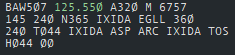
\includegraphics[width=0.65\textwidth]{img/labelsel.png}};
  %0,0-10.4-2.6

  \drawtag{2.3cm}{1.35,2.15}{callsign};
  \drawtagdesc{4cm}{0,4}{lcallsign}{L: Open \winref{menu:cs} \\R: Open Extended Tag};
  \draw[red,very thick] (callsign) -- (lcallsign);
  
  \drawtag{0.7cm}{3,2.15}{si};
  \drawtagdesc{2cm}{3.5,4}{lsi}{L: Open SI Menu\\R: Toggle SI Frequency};
  \draw[red,very thick] (si) -- (lsi);
  
  \drawtag{1.3cm}{4.3,2.15}{atyp};
  \drawtagdesc{3cm}{6.5,4}{latyp}{L: Toggle ATYP highlight\\R: Toggle ATYP display};
  \draw[red,very thick] (atyp) -- (latyp);

  \drawtag{0.4cm}{5.35,2.15}{wtc};
  \drawtagdesc{3cm}{10,4}{lwtc}{L: Toggle WTC highlight\\R: Toggle WTC display};
  \draw[red,very thick] (wtc.south east) -- (lwtc);
\end{tikzpicture}
\caption{Line 1 label Interaction}
\end{figure}

\note{Not shown in the above example: When \tagref{tag:PFREQ} is displayed R: Acknowledge PFREQ warning}

\subsubsection{Line 2}

\begin{figure}[H]
  \centering
\begin{tikzpicture}
  \node[anchor=south west,inner sep=0] at (0,0) {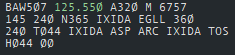
\includegraphics[width=0.65\textwidth]{img/labelsel.png}};

  \drawtag{1cm}{0.7,1.6}{afl};
  \drawtagdesc{2cm}{-1.5,1.6}{lafl}{L:Open \winref{menu:afl}};
  \draw[red,very thick] (afl) -- (lafl);

  \drawtag{1cm}{2,1.6}{cfl};
  \drawtagdesc{2cm}{-2,3.2}{lcfl}{L:Open \winref{menu:cfl}};
  \draw[red,very thick] (cfl) -- (lcfl);

  \drawtag{1.35cm}{3.35,1.6}{gs};
  \drawtagdesc{2cm}{0.5,4}{lgs}{L: Toggle GS highlight\\R: Toggle GS display};
  \draw[red,very thick] (gs) -- (lgs);

  \drawtag{1.7cm}{5.1,1.6}{NPT};
  \drawtagdesc{3cm}{3.5,4}{lnpt}{L: Open \winref{menu:wpt}\\R: Open \winref{win:dlcmw}};
  \draw[red,very thick] (NPT) -- (lnpt);

  \drawtag{1.35cm}{6.8,1.6}{ades};
  \drawtagdesc{3cm}{7,4}{lades}{L: Open \winref{win:fpw}\\R: Toggle ADES display};
  \draw[red,very thick] (ades) -- (lades);

  \drawtag{1cm}{8.2,1.6}{rfl};
  \drawtagdesc{3cm}{10.5,4}{lrfl}{L: Open \winref{menu:rfl}\\R: Open \winref{win:dlcmw}};
  \draw[red,very thick] (rfl) -- (lrfl);
\end{tikzpicture}
\caption{Line 2 label Interaction}
\end{figure}

\subsubsection{Line 3}

\begin{figure}[H]
  \centering
\begin{tikzpicture}
  \node[anchor=south west,inner sep=0] at (0,0) {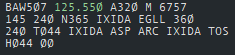
\includegraphics[width=0.65\textwidth]{img/labelsel.png}};

  \drawtag{1cm}{0.7,1.05}{xfl};
  \drawtagdesc{2cm}{-1.5,1.05}{lxfl}{L:Open XFL Menu};
  \draw[red,very thick] (xfl) -- (lxfl);

  \drawtag{1.35cm}{3.65,1.05}{ahdg};
  \drawtagdesc{2cm}{0.5,4}{lahdg}{L: Open \winref{menu:ahdg}};
  \draw[red,very thick] (ahdg) -- (lahdg);

  \drawtag{1cm}{5,1.05}{asp};
  \drawtagdesc{3cm}{3.5,4}{lasp}{L: Open \winref{menu:asp}\\R: Clear ASP value};
  \draw[red,very thick] (asp) -- (lasp);

  \drawtag{1cm}{6.25,1.05}{arc};
  \drawtagdesc{3cm}{7,4}{larc}{L: Open \winref{menu:arc}};
  \draw[red,very thick] (arc) -- (larc);

  \drawtag{1.35cm}{7.7,1.05}{copn};
  \drawtagdesc{3cm}{10.5,4}{lcopn}{L: Open \winref{menu:wpt}\\R: Toggle Flight Leg display};
  \draw[red,very thick] (copn) -- (lcopn);

  \drawtag{1.7cm}{9.4,1.05}{fcopx};
  \drawtagdesc{2cm}{12,1.05}{lfcopx}{R: Toggle Flight Leg display};
  \draw[red,very thick] (fcopx) -- (lfcopx);
\end{tikzpicture}
\caption{Line 3 label Interaction}
\end{figure}

\subsubsection{Line 4}

\begin{figure}[H]
  \centering
\begin{tikzpicture}
  \node[anchor=south west,inner sep=0] at (0,0) {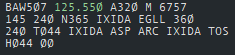
\includegraphics[width=0.65\textwidth]{img/labelsel.png}};

  \drawtag{1.35cm}{0.85,0.5}{dhdg};
  \drawtag{0.7cm}{2.1,0.5}{drc};
  \drawtagdesc{2cm}{1.5,-1}{ldap}{R: Toggle associated DAP display};
  \draw[red,very thick] (dhdg) -- (ldap);
  \draw[red,very thick] (drc) -- (ldap);
\end{tikzpicture}
\caption{Line 4 label Interaction}
\end{figure}

\subsubsection{Extended Label}

The Extended label is constructed of extra elements when compared to a Standard Selected label, some of which are interactable. These extra elements that are interactable are detailed below. The remaining elements function the same as in the Standard Selected label.

\begin{figure}[H]
  \centering
\begin{tikzpicture}
  \node[anchor=south west,inner sep=0] at (0,0) {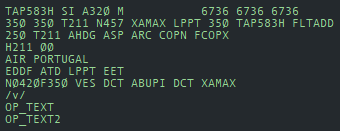
\includegraphics[width=0.65\textwidth]{img/labelext.png}};

  \drawtag{1cm}{7.65,3.7}{assr};
  \drawtagdesc{4cm}{10,5.5}{lassr}{L: Open \winref{menu:assr} \\R: Send Squawk CPDLC message};
  \draw[red,very thick] (assr) -- (lassr);
  
  \drawtag{0.7cm}{1.5,1.8}{atd};
  \drawtagdesc{2cm}{-2,4}{latd}{L: Open \winref{menu:tm}};
  \draw[red,very thick] (atd) -- (latd);
  
  \drawtag{1cm}{2.5,1.8}{ades};
  \drawtagdesc{3cm}{1.5,5.5}{lades}{L: Open \winref{win:fpw}\\R: Toggle ADES display};
  \draw[red,very thick] (ades) -- (lades);

  \drawtag{0.7cm}{3.5,1.8}{wtc};
  \drawtagdesc{3cm}{5.5,5.5}{lwtc}{L: Open \winref{win:fpw}};
  \draw[red,very thick] (wtc) -- (lwtc);

  \drawtag{1.7cm}{0.9,0.8}{opt};
  \drawtagdesc{3cm}{-2,2}{lopt}{L: Edit OP\_TEXT};
  \draw[red,very thick] (opt) -- (lopt);

  \drawtag{2cm}{1,0.25}{opt2};
  \drawtagdesc{2cm}{-2,0.6}{lopt2}{L: Edit OP\_TEXT2};
  \draw[red,very thick] (opt2) -- (lopt2);
\end{tikzpicture}
\caption{Extended Label Interaction}
\end{figure}

\subsubsection{Uncoupled Label}

\begin{figure}[H]
\centering
\begin{tikzpicture}
  \node[anchor=south west,inner sep=0] at (0,0) {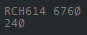
\includegraphics[width=0.2\textwidth]{img/labelunc.png}};

  \drawtag{1.2cm}{2.5,0.9}{callsign};
  \drawtagdesc{3.8cm}{1.6,2.3}{lcallsign}{L: Open \winref{menu:cs}};
  \draw[red,very thick] (callsign) -- (lcallsign);
  
  \drawtag{1.6cm}{0.95,0.9}{tssr};
  \draw[red,very thick] (tssr) -- (lcallsign);

\end{tikzpicture}
\caption{Uncoupled Label Interaction}
\end{figure}


\subsection{Label Compaction}
\label{tlabel:comp}

Label fields may be automatically supressed in certain conditions. This is called Label Compaction.

Label Compaction only occurs in unselected labels. When a field is supressed, the remaining fields to the right will move left to the supressed field position. If all fields in a line are supressed, the next line is moved up to the supressed line position. Values being coordinated are exempted from Label Compaction.

\bigskip

The following Label Compaction rules are in place:

\begin{itemize}
  \item If a field is empty it is supressed
  \item If AFL is the same as CFL, CFL is supressed
  \item If AFL is the same as CFL and XFL, CFL and XFL are supressed
  \item If AFL is the same as CFL, but different from XFL, only CFL is supressed
  \item If AFL is different from CFL, and CFL is the same as XFL, XFL is supressed
  \item If AFL is different from CFL, and CFL is different from XFL, no field is supressed
  \item If FCOPX is the same as NPT, NPT is supressed
\end{itemize}

\section{Track Label Menus}

These menus are opened from track label fields or flight lists. Except for the confirmation windows, they are closed automatically when a menu option is chosen or the mouse cursor leaves the menu area. Menu items shown with (X) represent an item that has an activated and a deactivated state. With the item activated, the item name is shown prefixed with the letter “X”. The mouse wheel can be used to scroll the selection lists in the menus.

\bigskip

Many of the menus have a default item or value, displayed with inverse video. The menu usually opens so that the default value is located under the mouse cursor for easy selection. Some menus contain items that open folders within the menu. They show a filled triangle before the item name (upright if the folder is closed, inverted if the folder is open). The “More” folder is opened automatically when the mouse cursor is placed over it or if the default item is in the “More” folder, other folders must be left-clicked to open.

\subsection{Callsign Menu}
\label{menu:cs}

\subsection*{Controlled Track}

\capdimage{img/cm.png}{Callsign Menu}

\begin{longtable}{p{5cm} p{7.5cm}}
Assume                    & Assumes track\\
Refuse                    & Refuses the incoming transfer\\
Transfer                  & Initiates a transfer to the next sector\\
Trf \& Release            & Opens the \winref{menu:xfrrel}\\
ROF                       & Sends a \winref{menu:rof}\\
(X)Freq                   & Toggles the \tagref{tag:Frequency dot}\\
(X)Highlight              & Toggles the Callsign highlight\\
(X)S-Highlight            & Toggles the Callsign+AFL fields highlight\\
PRL                       & Opens the \winref{menu:prl}\\
(X)Hold                   & “Hold” opens the \winref{menu:hold}, “XHold” cancels a given holding clearance\\
$\blacktriangledown$ More & Shows additional less frequently used options\\
Manual Transfer           & Opens the \winref{menu:mxfr}\\
(X)Inbound Est            & Toggles the “Inbound Est” manual alert\\
HOP                       & Initiates a \winref{win:hop}\\
(X)Mark                   & Toggles the \tagref{tag:Mark dot}\\
(X)Couple                 & Uncorrelates/correlates the flight plan\\
FPL…                      & Opens the \winref{win:fpw}\\
(X)Irregular              & Toggles the “Irregular” manual alert\\
Start/End CPDLC           & Starts/Ends CPDLC connection with the aircraft\\
VCI                       & Opens the \winref{menu:vci}\\
Squawk Ident              & Sends a “SQUAWK IDENT” CPDLC message to the aircraft\\
CPDLC Free Text           & Opens the \winref{menu:dlftm}\\
Free                      & Releases track\\
On Contact                & Sets track \stateref{On Contact}\footnotemark[1]\\
(X)Missed App             & Toggles the “Missed App” manual alert\\
\end{longtable}

\footnotetext[1]{Clicking “On Contact” for a track with “Y” or “Z” flight rules will also automatically change the flight rules in the VATSIM flight plan to VFR in order to make it uncontrolled. The displayed flight rules are not affected.}

\bigskip

Besides the manual alerts, none of the selectable toggle options in this menu will be transmitted to other controllers, but the “Mark”, “Freq” and highlight selections will be seen in your other EuroScope instances. A holding clearance is transmitted to the next controller when transferring the track. To correlate a flight plan, first click on the “Correlate” item, and then click on the radar position symbol of the desired radar track.

\bigskip

\subsection*{Uncontrolled Track}

\capdimage{img/cmuncon.png}{Uncontrolled Track Callsign Menu}

\begin{tabular}{l l l}
On Contact        & Sets track \stateref{On Contact} \\
Free              & Releases track\\
Assume            & Assumes track\footnotemark[1]\\
(X)Highlight      & Toggles the Callsign highlight\\
(X)S-Highlight    & Toggles the Callsign+AFL fields highlight\\
(X)Couple         & Uncorrelates/correlates the flight plan\\
(X)Hold           & “Hold” opens the \winref{menu:hold}, “XHold” cancels a given holding clearance\\
FPL...            & Opens the \winref{win:fpw}\\
PRL               & Opens the \winref{menu:prl}\\
\end{tabular}

\footnotetext[1]{Clicking “Assume” for a track with “Y” or “Z” flight rules will also automatically change the flight rules in the VATSIM flight plan to IFR in order to make it controlled. The displayed flight rules are not affected.}


\subsection*{Uncorrelated Track}

\capdimage{img/cmuncor.png}{Uncorrelated Track Callsign Menu}

\begin{tabular}{l l l}
Correlate       & Correlates the radar track with the next clicked “Callsign” field
\\Create APL    & Opens the \winref{win:apl}
\\PRL           & Opens the \winref{menu:prl}
\end{tabular}
\medskip

\subsection{Transfer menu}
\label{menu:xfr}

\capdimage{img/xfr.png}{Transfer Menu}

For CPDLC connected aircraft, the menu contains options related to the transfer. Left clicking on the frequency button initiates the transfer (and sends the CPDLC message if selected).

\bigskip

“Monitor” / “Contact” select which of the two CPDLC message types will be sent.

\bigskip

“R/T” / “CPDLC” select whether the transfer instruction is given via radio or as a CPDLC message.

\subsection{Transfer Confirmation Window}
\label{win:xfrconfirm}

\capdimage{img/xfrconfirm.png}{Transfer Confirmation Window}

If an aircraft has a defined XFL value and hasn’t been cleared to it (CFL is not equal to XFL), attempting to transfer the aircraft will open a Transfer Confirmation Window in the middle of the radar screen. While the window is open it will block all other attempts to click on items elsewhere on the radar screen. Either click on “Transfer” to transfer the aircraft regardless of the situation, or “Cancel” to cancel the transfer.

\subsection{Transfer \& Release menu}
\label{menu:xfrrel}

\capdimage{img/xfrrel.png}{Transfer \& Release menu}

The Transfer \& Release menu allows specifying a release condition for a track to be transferred. The transfer is initiated after selecting the desired condition (climb, descent, turn or full). The release will be shown on line 0 of the track label (C for climb, D for descent, T for turn and F for full). The transferring controller will see the label item until the track becomes unconcerned. The receiving controller will see the item for 3 minutes after the track is assumed.

\capdimage{img/xfrreldl.png}{CPDLC Transfer \& Release menu}

For CPDLC connected aircraft, the menu contains options related to the transfer:

\bigskip

“Monitor” / “Contact” select which of the two CPDLC message types will be sent.

\bigskip

“R/T” / “CPDLC” select whether the transfer instruction is given via radio or as a CPDLC message.

\warn{The “Trf \& Release” option will show the release condition on the downstream side only if the next controller is using this plugin, in other cases the transfer will be shown as a normal transfer.}

\subsection{Request On Frequency message}
\label{menu:rof}

See \winref{coo:rof}. For the message to succeed, you must be seen as the next controller for the tracking controller. When sent, the text “ROF” is displayed in the track label on the tracking controller’s screen.

\warn{The “ROF” message is a feature specific to this plugin. It is an experimental feature and is not guaranteed to work all the time. When you send the message, check that it’s sent properly.
\begin{enumerate}
        \item A successfully sent message will be displayed in the \winref{win:mow}
        \item If there is an error or the message fails to go through, a message will be put into the \winref{win:pqw}
\end{enumerate}}

\subsection{Hold Menu}
\label{menu:hold}

\capdimage{img/hold.png}{Hold Menu}

The Hold menu allows you to enter a holding clearance, adding the aircraft to the \winref{list:hold}. It displays for selection the points in the aircraft’s route that are ahead of its current position.

\bigskip

Left-clicking the empty box below the waypoint list opens a text entry box to enter any holding point name.

\bigskip

Left-clicking “Here” enters the present position coordinates as the holding point.

\bigskip

The holding point is automatically sent to your other EuroScope instances with a small delay and can be sent to other controllers by pushing the flight strip as the information is stored there.

\subsection{Manual Transfer Menu}
\label{menu:mxfr}

\capdimage{img/mxfr.png}{Manual Transfer Menu}

The Manual Transfer menu allows transferring the aircraft to any controller. In the SCHEDULED list are the controllers that are in the current sector sequence sorted in the order the aircraft is planned to enter the controllers’ sectors, with the next controller being the default item.

\bigskip

When opened, the “More” list displays all the other controllers for selection. Click on a controller ID to start the transfer. For CPDLC connected aircraft, clicking on a controller ID opens the \winref{menu:xfr}

\subsection{VCI Menu}
\label{menu:vci}

\capdimage{img/vci.png}{VCI Menu}

Available only for CPDLC-connected aircraft and when more than one frequency has been set up by the controller, the VCI menu allows sending a CPDLC “contact” or “monitor” message without initiating a transfer.

\bigskip

The first button displays the primary frequency, left-clicking it will send the message with that frequency.

\bigskip

Left-clicking the “Select Freq” button will open a text entry box to enter any other frequency. If a valid frequency (set up as XMT TXT in EuroScope’s Voice communication setup dialog) is entered, the message will be sent with that frequency.

\bigskip

“Monitor” and “Contact” are used to select the type of message to be sent.

\subsection{CPDLC Free Text Menu}
\label{menu:dlftm}

See \winref{cpdlc:freetext}. Left-clicking on a message sends it.

\bigskip

The menu closes when a message is sent or the cursor leaves the menu area.

\subsection{Prediction Line Menu}
\label{menu:prl}

\capdimage{img/prl.png}{Prediction Line Menu}

The Prediction Line menu allows displaying a PRL with a specific length for each aircraft even if the PRL selection is off in the Radar Menu.

\bigskip

The default value is the set PRL value if available, otherwise the PRL length value from the Track Control Window. Changing the PRL length value in the \winref{win:tcw} or changing the PRL setting in the \winref{menu:radarm} will delete all manually set PRL lengths.

\subsection{Sequence Number Menu}
\label{menu:seq}

\capdimage{img/seq.png}{Sequence Number Menu}

This menu is used to set an arrival sequence number. Values from 1 to 50 are available.

\bigskip

\warn{The sequence number will not be transmitted to other controllers except the next controller (during transfer) unless the flight strip is manually sent.}

\subsection{Waypoint Menu}
\label{menu:wpt}

\capdimage{img/wpt.png}{Waypoint Menu}

\begin{longtable}{p{5cm} p{7.5cm}}
$\blacktriangle$  Routing & Opens the “COPN point” or “COPX point” submenu (EuroScope default item)\\
$\blacktriangle$ Arrival & Opens the “Assign STAR” submenu (EuroScope default item)\\
$\blacktriangle$ Departure & Opens the “Assign SID” submenu (EuroScope default item)\\
$\blacktriangle$ TSA Hold & Opens the TSA Hold submenu (not available if a holding clearance is active)\\
$\blacktriangle$ Hold & Opens the Hold submenu (not available if a TSA holding clearance is active)\\
\end{longtable}

\bigskip

This menu gives access to functions related to the route of the aircraft. It is used to assign direct-to clearances, departure and arrival routes, holding clearances, and to coordinate the sector entry/exit point.

\capdimage{img/wptyn.png}{Waypoint Menu in Coordination}

When an entry or exit coordination has been received, the menu opens looking like this instead. The options are:

\begin{longtable}{p{5cm} p{7.5cm}}
$\blacktriangle$ Routing    & Opens the “COPN point” or “COPX point” submenu (EuroScope default item)
\\Accept                      & Accepts the coordination
\\Reject                      & Rejects the coordination
\end{longtable}

The submenu opened with “Routing” offers the same possibilities to accept or reject the coordination, but also the possibility to counter-propose a different point.

\capdimage{img/wptdl.png}{CPDLC DCT Request Downlink Waypoint Menu}

When the aircraft is CPDLC-connected and the coordination is an exit coordination, the menu offers a choice between “R/T” and “CPDLC”. The chosen option decides how an accepted coordination is communicated to the aircraft.

\bigskip

With “CPDLC” selected, when “Accept” is clicked, in addition to the coordination being accepted, a “PROCEED DIRECT TO <point>” CPDLC message is sent to the aircraft.

\capdimage{img/wptroute.png}{CPDLC Waypoint Menu}

When a direct-to downlink request has been received, the menu can be used to answer it.

\bigskip

\begin{longtable}{p{5cm} p{7.5cm}}
Point name  & Sends a “PROCEED DIRECT TO <point>” CPDLC message\\
SBY         & Sends a “STANDBY” CPDLC message\\
UNABLE      & Sends an “UNABLE” CPDLC message\\
\end{longtable}   

\bigskip

The “R/T” / “CPDLC” selection is fixed to “CPDLC”.

\warn{Clicking the point name will set the direct-to clearance without coordination}

When there is no request in process and the aircraft has a direct-to point set, the menu can be used to send the clearance via CPDLC. In this case the menu opens like this except without the “SBY” and “UNABLE” buttons. Clicking the point name will send the “PROCEED DIRECT TO <point>” CPDLC message.

\subsection*{TSA Hold Submenu}

The TSA Hold submenu allows you to enter a clearance to enter an active military area. It displays the active and preactive TSA type areas. If a clearance already exists, the menu will only give the option to remove it with the “XHold” item.

\bigskip

The clearance is automatically sent to your other EuroScope instances with a small delay and can be sent to other controllers by pushing the flight strip as the information is stored there. A TSA hold clearance will exclude the aircraft from all APW and SAP processing.

\subsection*{TSA Hold Submenu}

If a holding clearance already exists, the menu will only give the option to remove it with the “XHold” item.
See \winref{menu:hold} for other details.

\subsection{AFL Menu}
\label{menu:afl}

\begin{center}
  \begin{minipage}[b]{0.14\textwidth}\end{minipage}\hfill 
  \begin{minipage}[b]{0.14\textwidth}\capdimage{img/afl.png}{AFL Menu nautical units}\end{minipage}\hfill 
  \begin{minipage}[b]{0.14\textwidth}\capdimage{img/aflm.png}{AFL Menu metric units}\end{minipage}\hfill  
  \begin{minipage}[b]{0.14\textwidth}\capdimage{img/kbd.png}{AFL Menu keyboard}\end{minipage}\hfill 
  \begin{minipage}[b]{0.14\textwidth}\end{minipage}\hfill 
\end{center}  

This menu can be used to set the AFL value for aircraft that don’t have an altitude reporting transponder.

\bigskip

The default value is the previously set manual AFL value if set, otherwise the CFL value.

\bigskip

By default, the menu (as well as the AFL label item) is always showing nautical units, regardless of the system units or the selected units for the aircraft. If this behavior is selected off, the list units can be toggled with the “NAUTICAL” / “METRIC” item. There are three ways to set the AFL using this menu:

\bigskip

\begin{itemize}
        \item Clicking a level value in the list
        \item Clicking the text entry box below the level list and entering the value there
        \item Clicking the right-pointing triangle to open a keyboard that can be used to type in the value using the mouse. “C” clears the entry and “Ok” sets the value.
\end{itemize}

\bigskip

Entering a metric value will also set the aircraft’s units to metric; a nautical value will set nautical units.

\bigskip

The accepted manual level entry formats for the AFL, CFL and RFL menus are as follows (“n” is a number):

\bigskip

\begin{longtable}{p{5cm} p{7.5cm}}
“Annn” or “nnn”         & Altitude in hundreds of feet\\
“Mnnnn” or “nnnn”       & Altitude in tens of meters\\
“Mnnnnn” or “nnnnn”     & Altitude in meters\\
“Ennn”                  & Height in hundreds of feet above aerodrome elevation\\
“Ennnn”                 & Height in tens of meters above aerodrome elevation\\
“Ennnnn”                & Height in meters above aerodrome elevation\\
\end{longtable}    

\bigskip

Regardless of whether the entered value is in meters or feet, and altitude or height, it will be converted to altitude in feet and the result is then rounded to the nearest 100 feet.

\subsection{CFL Menu}
\label{menu:cfl}
\capdimage{img/cfl.png}{CFL Menu}

In the track label the CFL menu is combined with the COPN altitude coordination menu and the CFL menu opens only when the aircraft is assumed. The default value is by default the XFL, but it can be changed to the current CFL or the RFL in the \winref{menu:localset}. Altitudes up to the transition altitude are prefixed with “A” in the nautical units list and with “M” in the metric units list. QFE heights are prefixed with “E” in both lists. Selectable values are from 500ft to FL650 with 500ft intervals up to the transition altitude, then 1000ft intervals up to FL410 and 2000ft intervals above it. 

\bigskip

“Visual App” / “VA” and “Clear for App” / “CA” set the corresponding approach clearances.

\bigskip

The list units can be toggled with the “NAUTICAL” / “METRIC” item. There are three ways to set the CFL using this menu:

\bigskip

\begin{itemize}
        \item Clicking a level value in the list or one of the two approach clearance items
        \item Clicking the text entry box between the level list and the approach clearance item and entering the value there
        \item Clicking the right-pointing triangle to open a keyboard that can be used to type in the value using the mouse. “C” clears the entry and “Ok” sets the value.
\end{itemize}

\bigskip

Entering a metric value will set the aircraft’s units to metric; a nautical value will set nautical units.

\bigskip

The aircraft’s RFL is displayed in the place of the “NAUTICAL”/”METRIC” item with format “R<RFL>”. Left-clicking the button still has the same effect (changes the displayed units).

\capdimage{img/cfldl.png}{CPDLC CFL Menu}

For CPDLC connected aircraft, the menu contains “R/T” and “CPDLC” options to select whether a level clearance is to be sent via radio or as a CPDLC message.

\bigskip

If a level request has been received from the aircraft, there are also “SBY” and “UNABLE” buttons to send those messages as a reply.

\bigskip

- When a level request downlink has been received, the “R/T” option is deselected and cannot be selected. The request must be replied to using CPDLC.

\bigskip

- When a level clearance uplink has been sent, the “CPDLC” option is deselected and cannot be selected. If a new level clearance must be sent before there is an answer to the uplink, it must be given via radio (doing so also closes the open uplink message).

\subsection{RFL Menu}
\label{menu:rfl}

The RFL menu allows setting the requested flight level. The operation is similar to the AFL and CFL menus. The function for the “NEXT” button is not implemented.

\subsection{AHDG Menu}
\label{menu:ahdg}

\capdimage{img/ahdg.png}{AHDG Menu}

This menu includes items to set or clear an assigned heading or a direct route and to send a HOP. The initially highlighted heading value will be the closest one to the assigned heading if the aircraft has one, otherwise the closest one to the aircraft ground track, or the departure runway heading if the menu is opened from the \winref{list:dep}. Clicking on a heading value will set it as the assigned heading. The assigned heading can also be set by typing it into the entry box, using the pop-up keyboard or by using the AHDG vector.

\bigskip

“Clear” removes an assigned heading or a direct route. For CPDLC connected aircraft, it sends the “RESUME OWN NAVIGATION” CPDLC message if the “CPDLC” option is selected.

\bigskip

“Point” lets you pick a direct-to point from the radar screen. Left-click on any point to set it as the direct-to point (available points are VORs, NDBs and waypoints, in that priority order). Pressing the [Esc] key or clicking on any clickable data field will abort the operation.

\bigskip

“HOP”, “RTI” and “TIP” are coordination functions (see \winref{win:hop}, \winref{win:rti}). To use them, first click on the function’s button and then select the desired value from the list (for HOP also “Point” is available).

\bigskip

\capdimage{img/ahdgdl.png}{CPDLC AHDG Menu}

\bigskip

For CPDLC connected aircraft, the menu contains additional buttons:

\bigskip

“R/T” and “CPDLC” select whether a heading/direct-to clearance is to be sent via radio or as a CPDLC message.

\bigskip

\begin{itemize}
        \item When a heading request downlink has been received, the “R/T” option is deselected
    and cannot be selected. The request must be replied to using CPDLC.
        \item When a heading/direct-to clearance uplink has been sent, the “CPDLC” option is deselected and cannot be selected. If a new heading/direct-to clearance must be sent before there is an answer to the uplink, it must be given via radio (doing so also closes the open uplink message).
\end{itemize}

\bigskip

“SBY” and “UNABLE” send the corresponding answers to a downlink heading request
message.

\warn{Clicking a point on the radar screen will set the direct-to clearance without coordination }

\subsection{Handover Proposal (HOP)}
\label{win:hop}

See \winref{coo:hop}. For the receiving controller a HOP is identified by coloring the \tagref{tag:CALLSIGN} field with \colorref{Proposition In} color in the label. For the sending controller the \tagref{tag:CALLSIGN} field remains \colorref{Assumed} color and the \tagref{tag:SI} field is shown in \colorref{Proposition In} color. Additionally, if there are proposed parameters they are also colored \colorref{Proposition In} in both controllers’ labels.

\bigskip

There are three ways to answer a HOP and all of them involve accepting all proposed parameters. If one or more parameters are not acceptable, coordination must be done to find acceptable parameters or to revert to standard ones. The available ways, in order of preference, to accept the proposed parameters are:

\bigskip

\begin{longtable}{p{5cm} p{7.5cm}}
  \winref{menu:cs} -> “ROF”               & Sends a Request On Frequency message\\
  \winref{menu:ctm} -> “Accept”      & Sends an Accept message\\
  \winref{menu:cs} -> “Assume”            & Assumes the track\\
\end{longtable}

\bigskip

If the parameters are unacceptable to the receiving controller, the sending controller has the possibility to modify or clear them using the appropriate menus, or to cancel the whole HOP by assuming the track.

\warn{A HOP will only be shown correctly for controllers using this plugin. To other controllers it will be shown as a normal transfer without any special coloring of any data fields. This combined with the three possible ways to answer the HOP require the sending controller to pay special attention to the track to see what the result is.}

\warn{If a HOP is sent to a manually selected controller, the next controller selection will be reset to the automatically calculated controller when an “ROF” or “Accept” answer is received. The correct controller must then be manually selected again for the transfer.}

\subsection{Request Tactical Instructions (RTI) / Tactical Instructions Proposal (TIP)}
\label{win:rti}
\label{win:tip}

Certain tactical data (AHDG, ASP and ARC) can be coordinated using the \winref{coo:rti} functions. Their only difference is that RTI is used for requesting the parameters when the aircraft is inbound to your sector and your sector is the next in the sector sequence, and TIP to propose the parameters to the next sector when the aircraft is assumed. Contrary to the \winref{win:hop} function, these coordinations can be refused using the system, and they do not offer the aircraft for transfer.

\bigskip

When sent, the RTI/TIP is displayed on both controllers’ screens by displaying the requested parameter on line 0 of the track label in \colorref{Proposition In} color.

\bigskip

To answer the RTI/TIP, left-click on the requested parameter on line 0 of the track label or the corresponding message in the \winref{win:miw}. This will open the \winref{menu:ttm}.

\warn{The “RTI” and “TIP” messages are features specific to this plugin. They are experimental features not guaranteed to work all the time. When you send these messages, check that they are sent properly.

\bigskip

\begin{itemize}
        \item A successfully sent message will be displayed in the \winref{win:mow} and the requested parameter being shown above the track label
        \item If there is an error or the message fails to go through, a message will be put into the \winref{win:pqw}.
\end{itemize}}

\subsection{AHDG Vector}
\label{menu:ahdgv}
The AHDG vector is another way of setting an assigned heading for an aircraft. To use the vector, left-click on the radar position symbol of the aircraft. This will start drawing the vector. When you’re satisfied with the heading value, left-click again to set it. Right-clicking will abort drawing the vector.

\bigskip

When the cursor is over a known point (VOR, NDB or waypoint), the name of that point is displayed instead of the heading value, and left-clicking will set a direct-to clearance to that point. To temporarily disable the known points functionality, keep the <ALT> key pressed while using the vector.

\subsection{ARC Menu}
\label{menu:arc}

\capdimage{img/arc.png}{ARC Menu}

The ARC menu allows assigning a rate of climb or descent to the flight plan. Selectable rates are 500-5000 ft/min (displayed in 100’s of ft/min), or 5-25 m/s. The menu units are always the same as the units used for the aircraft in general.

\bigskip

Left-clicking on a value assigns it. An assigned rate can be cleared by selecting the “Resume” item.

\bigskip

By default, the “+” option is selected, meaning that the clearance is a minimum rate of climb or descent. Deselecting the “+” makes the clearance an exact rate, and selecting the “-” option makes the clearance a maximum rate.

\bigskip

“RTI” and “TIP” are coordination functions (see \winref{win:rti}). To use them, first click on the function’s button and then select the desired value from the list.

\warn{The exact and maximum rate clearances are a feature specific to this plugin (the additional information is stored in the flight strip). To controllers not using TopSky, all assigned rate clearances will only show the rate value.

Assigned rate clearances given by controllers not using TopSky will be displayed as minimum rate clearances. }

\subsection{ASP Menu}
\label{menu:asp}

\begin{center}
  \begin{minipage}[b]{0.14\textwidth}\end{minipage}\hfill 
  \begin{minipage}[b]{0.14\textwidth}\capdimage{img/asp.png}{ASP Menu}\end{minipage}\hfill 
  \begin{minipage}[b]{0.14\textwidth}\capdimage{img/aspmach.png}{ASP Menu Mach option}\end{minipage}\hfill  
  \begin{minipage}[b]{0.14\textwidth}\end{minipage}\hfill 
\end{center} 

\bigskip

The ASP menu allows setting an assigned speed or Mach number. The default value will be the closest value to the assigned one if set, otherwise TopSky will suggest the closest value to the aircraft’s present speed based on the ground speed (zero wind will be assumed). The menu will initially open in IAS mode if the aircraft’s CFL is below FL285, and in Mach mode if above it. The selectable values range from 100 to 400 knots and from M0.50 to M1.00.

\bigskip

The “+” and “-” options can be used to specify the clearance
as a minimum/maximum speed.

\bigskip

The “Resume” item clears an assigned value. For CPDLC connected aircraft, it sends the “RESUME NORMAL SPEED” CPDLC message if the “CPDLC” option is selected.

\bigskip

When the “Resume” button below the list is replaced by a “HS” button, clicking it will set a clearance for “high speed”, displayed as “HS” in the ASP label field. For CPDLC connected aircraft, it sends the “NO SPEED RESTRICTION” CPDLC message if the “CPDLC” option is selected. The “Resume” button can be found at the bottom of the “More” list.

\bigskip

“HOP”, “RTI” and “TIP” are coordination functions (see \winref{win:hop}, \winref{win:rti}). To use them, first click on the function’s button and then select the desired value from the list (for HOP also “Point” is available).

\bigskip

Entering a metric value will set the aircraft’s units to metric, a nautical value will set nautical units.

\bigskip

\capdimage{img/aspmachdl.png}{CPDLC ASP Menu}
For CPDLC connected aircraft, the menu contains additional buttons:

\bigskip

R/T” and “CPDLC” select whether a speed clearance is to be sent via radio or as a
CPDLC message.

\bigskip

\begin{itemize}
    \item When a speed request downlink has been received, the “R/T” option is deselected and cannot be selected. The request must be replied to using CPDLC.
    \item When a speed clearance uplink has been sent, the “CPDLC” option is selected and cannot be deselected. If a new speed clearance must be sent before there is an answer to the uplink, it must be given via radio (doing so also closes the open uplink message).
\end{itemize}

\bigskip

SBY” and “UNABLE” send the corresponding answers to a downlink speed request.

\warn{The minimum and maximum speed clearances are a feature specific to this plugin (the additional information is stored in the flight strip). To controllers not using TopSky, all assigned speed clearances will only show the speed value. Assigned speed clearances given by controllers not using TopSky will be displayed as exact speed clearances.}

\subsection{ASSR Menu}
\label{menu:assr}
\capdimage{img/assr.png}{ASSR Menu}

The ASSR menu allows assigning an SSR code to the flight plan. To enter a new code, type it by left-clicking the numbers. “C” clears the entered value and “Ok” assigns the code if it’s a valid one. To get an automatically assigned code, clear the value and then left-click on “Ok” with the entry box left empty.

%\bigskip
%
%Depending on the configuration, the assigned code may be a mode S conspicuity code. To force a discrete code, make a new assignment – either manual or automatic. If an automatic assignment is requested for a flight with the conspicuity code currently assigned, the new assignment will be a discrete code.
%
\subsection{Combined Transfer Menu}
\label{menu:ctm}
\capdimage{img/ctm.png}{Combined Transfer Menu}

The Combined Transfer menu displays the proposed transfer parameters for a \winref{coo:hop}. It is opened by clicking on the \tagref{tag:AHDG}, \tagref{tag:ASP} or \tagref{tag:COPN/COPX} items in the track label or flight list, or the list row displaying the HOP message in the \winref{win:miw}.

\bigskip

From top to bottom, the displayed values are the direct-to point, speed/Mach value, and the assigned heading value. If one or more of them are not proposed, the value will be replaced by the string “none” (the image above shows the menu for a HOP without any proposed parameters). Clicking on “Accept” will send a message to the upstream controller that the proposed parameters, if any, are all acceptable.

\subsection{Tactical Transfer Menu}
\label{menu:ttm}
\capdimage{img/ttm.png}{Tactical Transfer Menu}

The Tactical Transfer menu is used to accept, reject or apply tactical data (\tagref{tag:AHDG}, \tagref{tag:ASP} and/or \tagref{tag:ARC}). It is opened by left-clicking on a proposed or accepted parameter in the track label. The menu displays all proposed (in \colorref{Proposition In} color) and accepted (in sector state color) values.

\bigskip

Clicking on “Accept” will accept all proposed values and “Reject” will reject them. The menu is then closed.

\bigskip

Once a value is accepted, the respective label field will be colored \colorref{Information} until the value is set to the accepted one.
\bigskip

Note that the menu displays both sent and received coordinations, but you can naturally only accept/reject the received ones and apply values for aircraft that are assumed.

\bigskip

All tactical data coordinations (also any rejected ones) can be viewed in the \winref{win:tiw}, but they cannot be answered or applied there.

\subsection{Aerodrome Menu}
\label{menu:ad}
\capdimage{img/ad.png}{Aerodrome Menu}

The Aerodrome menu is used to select the aerodrome(s) for aerodrome related windows and functions. The list contains all aerodromes with runways defined in the active sector file. To select an aerodrome, left-click on it or type its identifier into the text entry box below the list.

\bigskip

Selection of more than one aerodrome is possible when the menu was opened from the \winref{win:wxmw}. In this case the “All” button is available and clicking on it will select all the aerodromes in the list.

\bigskip

Clicking on “Ok” will confirm the selection(s) and close the menu.

\subsection{NPT Menu}
\label{menu:npt}
\capdimage{img/npt.png}{NPT Menu}

The NPT menu is used to answer a direct-to downlink request using CPDLC. The menu
contains three options:

\bigskip

\begin{longtable}{p{5cm} p{7.5cm}}
Point name  & Sends a “PROCEED DIRECT TO <point>” CPDLC message\\
SBY         & Sends a “STANDBY” CPDLC message\\
UNABLE      & Sends an “UNABLE” CPDLC message\\   
\end{longtable}

\bigskip

The menu closes when an option is selected or the cursor leaves the menu area. If the aircraft cannot be cleared direct to the requested point but to another one, the request must be answered with “UNABLE” and a separate direct-to clearance must be given.

\warn{Clicking the point name will set the direct-to clearance without coordination}

\subsection{CPDLC Emergency Acknowledgement Menu}
\label{menu:dleam}
\capdimage{img/dlmayday.png}{CPDLC Emergency Acknowledgement Menu}

When a CPDLC emergency message has been received, this menu is used to respond to it (if applicable), and then acknowledge the situation. When a reply is required, the menu button will read “ROGER”. Left-clicking on it will send the “ROGER” CPDLC message and close the menu. When opening the menu again (or when a reply was not required), the button reads “Ack”. Left-clicking on it will acknowledge the emergency. 

\bigskip

The menu is closed when the “ROGER”/“Ack” button is clicked or the cursor leaves the menu area.

\subsection{CPDLC Pilot Late Acknowledgement Menu}
\label{menu:dlplam}
\capdimage{img/dlplate.png}{CPDLC Pilot Late Acknowledgement Menu}

When there is no answer to a CPDLC uplink clearance, this menu can be used to resolve the situation. “Abort” discards the uplink and “Manual WILCO” simulates reception of a WILCO message.

\subsection{Time Menu}
\label{menu:tm}
\capdimage{img/etd.png}{Time Menu}

The Time menu is used to set/change the time value for ATD, EOBT, ETD and SLOT fields.
Default values are:

\begin{longtable}{p{5cm} p{7.5cm}}
ATD     & Current time\\
EOBT    & Current time\\
ETD     & Current field value\\
SLOT    & Current field value if any (ATD if different from ETD), current time otherwise\\
\end{longtable}

The up/down arrows are used to change the value, “Ok” sets the time.

\subsection{Departure Sequence Menu}
\label{menu:dqm}
\capdimage{img/dsq.png}{Departure Sequence Menu}

The DSQ menu is used to select a specific departure sequence number to a flight. The list includes the possible numbers, and the current number is highlighted. Left-clicking on a number sets it, “Clear” removes the flight from the departure sequence.

\note{The departure sequence number is only stored locally, it is not sent to other controllers or even to other EuroScope instances.}

\section{Aircraft Lists}

\subsection{Departure List}
\label{list:dep}

The Departure List contains all departures still on the ground of the controlled aerodromes.

\begin{longtable}{|p{0.25\textwidth}|p{0.25\textwidth}|p{0.25\textwidth}|p{0.10\textwidth}|} \hline
  \textbf{Item}                 & \textbf{Left Mouse}                 & \textbf{Right Mouse}      & \textbf{Default Visibility}  \endhead \hline
  \tagref{tag:CALLSIGN}         & Open \winref{menu:cs}               & Toggle Flight Leg display & \usym{2713}         \\ \hline
  \tagref{tag:EOBT}             & Edit EOBT                           & Edit EOBT                 &                     \\ \hline
  \tagref{tag:TOBT}             & Edit TOBT                           & Edit TOBT                 & \usym{2713}         \\ \hline
  \tagref{tag:TSAT}             & Ready TOBT                          & Set TOBT to now           & \usym{2713}         \\ \hline
  \tagref{tag:TSAC}             & Add TSAT to TSAC                    & Edit TSAC                 &                     \\ \hline
  \tagref{tag:ASRT}             & Toggle ASRT                         & Toggle ASRT               &                     \\ \hline
  \tagref{tag:ASAT}             &                                     &                           &                     \\ \hline
  \tagref{tag:TTOT}             &                                     &                           &                     \\ \hline
  \tagref{tag:CTOT}             & Open CTOT Option list               & Open CTOT Option list     &                     \\ \hline
  \tagref{tag:Flow Message}     & Open \winref{menu:ahdg}             &                           &                     \\ \hline
  \tagref{tag:Ready}            & Toggle Ready                        &                           &                     \\ \hline
  \tagref{tag:ATYP}             &                                     &                           & \usym{2713}         \\ \hline
  \tagref{tag:WTC}              &                                     &                           & \usym{2713}         \\ \hline
  \tagref{tag:V}                &                                     &                           & \usym{2713}         \\ \hline
  \tagref{tag:Departure stand}  &                                     &                           & \usym{2713}         \\ \hline
  QNH                           & Edit OP TEXT                        & Edit OP TEXT              &                     \\ \hline
  \tagref{tag:ADEP}             & Open \winref{win:fpw}               & Toggle Flight Leg display & \usym{2713}         \\ \hline
  \tagref{tag:ADES}             & Open \winref{win:fpw}               & Toggle Flight Leg display & \usym{2713}         \\ \hline
  \tagref{tag:DRWY}             & Open \winref{win:dlpdcw}            & Open \winref{win:dlpdcw}  & \usym{2713}         \\ \hline
  \tagref{tag:SID}              & Open \winref{win:dlpdcw}            & Open \winref{win:dlpdcw}  & \usym{2713}         \\ \hline
  \tagref{tag:ASSR}             & Open \winref{menu:assr}             & Open \winref{menu:assr}   & \usym{2713}         \\ \hline
  \tagref{tag:CFL}              & Open \winref{menu:cfl}              & Open \winref{menu:cfl}    & \usym{2713}         \\ \hline
  \tagref{tag:RFL}              & Open \winref{menu:rfl}              & Open \winref{menu:rfl}    & \usym{2713}         \\ \hline
  \tagref{tag:CLR}              & Toggle Clearance Acknowledged flag  &                           & \usym{2713}         \\ \hline
  \tagref{tag:Ground state}     & Open Ground State Menu              & Open Ground State Menu    & \usym{2713}         \\ \hline
  \tagref{tag:OP TEXT2}         & Edit OP TEXT2                       & Edit OP TEXT2             & \usym{2713}         \\ \hline
  \caption{Departure List Construction}
\end{longtable}

\subsection{Sector List}
\label{list:sector}

\winref{menu:global} Tools -> Flight Plan Lists -> Sector List…

The Sector List contains all departed controlled aircraft in the following states:

\bigskip

\begin{itemize}
    \item Informed\footnotemark[1]
    \item Concerned\footnotemark[1]\footnotemark[2]
    \item Coordinated
    \item Transfer to me initiated
    \item Assumed
    \item Transfer from me initiated
    \item Redundant\footnotemark[1]
\end{itemize}

\footnotetext[1]{If corresponding selection made in the Global menu}

\footnotetext[2]{The display of concerned aircraft is limited to those entering the sector within 60 minutes}

\begin{longtable}{|p{0.25\textwidth}|p{0.25\textwidth}|p{0.25\textwidth}|p{0.10\textwidth}|} \hline
  \textbf{Item}         & \textbf{Left Mouse}     & \textbf{Right Mouse}      & \textbf{Default Visibility}  \endhead \hline
  \tagref{tag:CALLSIGN} & Open \winref{menu:cs}   & Open Extended Label       & \usym{2713}         \\ \hline
  \tagref{tag:ETN}      &                         &                           & \usym{2713}         \\ \hline
  \tagref{tag:PEL}      & Open PEL Menu           &                           & \usym{2713}         \\ \hline
  \tagref{tag:COPN}     & Open \winref{menu:wpt}  & Toggle Flight Leg display & \usym{2713}         \\ \hline
  \tagref{tag:NRAC}     &                         &                           &                     \\ \hline
  \tagref{tag:ATYP}     &                         &                           & \usym{2713}         \\ \hline
  \tagref{tag:WTC}      &                         &                           &                     \\ \hline
  \tagref{tag:V}        &                         &                           &                     \\ \hline
  \tagref{tag:CFL}      & Open \winref{menu:cfl}  &                           & \usym{2713}         \\ \hline
  \tagref{tag:AHDG}     & Open \winref{menu:ahdg} &                           &                     \\ \hline
  \tagref{tag:ASP}      & Open \winref{menu:asp}  & Clear ASP value           &                     \\ \hline
  \tagref{tag:TAS}      &                         &                           &                     \\ \hline
  \tagref{tag:ETX}      &                         &                           &                     \\ \hline
  \tagref{tag:XFL}      & Open XFL Menu           &                           &                     \\ \hline
  \tagref{tag:COPX}     & Open \winref{menu:wpt}  &                           &                     \\ \hline
  \tagref{tag:RFL}      & Open \winref{menu:rfl}  &                           &                     \\ \hline
  \tagref{tag:ASSR}     & Open \winref{menu:assr} & Send CPDLC Squawk message &                     \\ \hline
  \tagref{tag:NSSR}     & Open \winref{menu:assr} & Send CPDLC Squawk message &                     \\ \hline
  \tagref{tag:ADEP}     &                         &                           &                     \\ \hline
  \tagref{tag:SID}      & Open SID list           &                           & \usym{2713}         \\ \hline
  \tagref{tag:DRWY}     & Open Runway list        &                           &                     \\ \hline
  \tagref{tag:FCOPX}    &                         & Toggle Flight Leg display &                     \\ \hline
  \tagref{tag:ETX}      &                         &                           &                     \\ \hline
  \tagref{tag:ADES}     & Open \winref{win:fpw}   &                           & \usym{2713}         \\ \hline
  \tagref{tag:SI}       & Open SI list            & Toggle SI frequency       &                     \\ \hline
  \tagref{tag:ADES}     & Open \winref{win:fpw}   &                           & \usym{2713}         \\ \hline
  \tagref{tag:ETA}      &                         &                           & \usym{2713}         \\ \hline
  \tagref{tag:STAR}     & Open STAR list          &                           & \usym{2713}         \\ \hline
  \tagref{tag:ARWY}     & Open Runway list        &                           & \usym{2713}         \\ \hline
  \tagref{tag:OP TEXT}  & Edit OP\_TEXT           &                           & \usym{2713}         \\ \hline
  \tagref{tag:OP TEXT2} & Edit OP\_TEXT2          &                           & \usym{2713}         \\ \hline
  \caption{Sector List Construction}
\end{longtable}

\subsection{Load Factor List}
\label{list:load}

\winref{menu:global} Tools -> Flight Plan Lists -> Load Factor List…

\bigskip

The Load Factor List contains all departed controlled aircraft in the concerned state and all non-departed controlled aircraft in the concerned and coordinated states expected to enter the sector within 4 hours.

\begin{longtable}{|p{0.25\textwidth}|p{0.25\textwidth}|p{0.25\textwidth}|p{0.10\textwidth}|} \hline
  \textbf{Item}         & \textbf{Left Mouse}     & \textbf{Right Mouse}      & \textbf{Default Visibility}  \endhead \hline
  \tagref{tag:CALLSIGN} & Open \winref{menu:cs}   & Open Extended Label       & \usym{2713}         \\ \hline
  \tagref{tag:ETN}      &                         &                           & \usym{2713}         \\ \hline
  \tagref{tag:PEL}      & Open PEL Menu           &                           & \usym{2713}         \\ \hline
  \tagref{tag:COPN}     & Open \winref{menu:wpt}  & Toggle Flight Leg display & \usym{2713}         \\ \hline
  \tagref{tag:ADEP}     &                         &                           & \usym{2713}         \\ \hline
  \tagref{tag:ADES}     & Open \winref{win:fpw}   &                           & \usym{2713}         \\ \hline
  \tagref{tag:RFL}      & Open \winref{menu:rfl}  & Open \winref{win:dlcmw}   & \usym{2713}         \\ \hline
  \tagref{tag:ASSR}     & Open \winref{menu:assr} & Send CPDLC Squawk message & \usym{2713}         \\ \hline
  \caption{Load Factor List Construction}
\end{longtable}  

\subsection{Uncontrolled Lists}
\label{list:uncon}

\winref{menu:global} Tools -> Flight Plan Lists -> Uncontrolled List 1/2…

\bigskip

The Uncontrolled List contains all or a subset of Uncontrolled aircraft, depending on whether filters are set up.

\bigskip

Up to 2 lists can be displayed. Each list may be configured with different filtering options.

\begin{longtable}{|p{0.25\textwidth}|p{0.25\textwidth}|p{0.25\textwidth}|p{0.10\textwidth}|} \hline
  \textbf{Item}         & \textbf{Left Mouse}           & \textbf{Right Mouse}      & \textbf{Default Visibility}  \endhead \hline
  \tagref{tag:CALLSIGN} & Open \winref{menu:cs}         & Open Extended Label       & \usym{2713}         \\ \hline
  \tagref{tag:ASSR}     & Open \winref{menu:assr}       & Send CPDLC Squawk message & \usym{2713}         \\ \hline
  \tagref{tag:ADEP}     &                               &                           & \usym{2713}         \\ \hline
  \tagref{tag:ATD}      & Open \winref{menu:tm}         &                           & \usym{2713}         \\ \hline
  \tagref{tag:ADES}     & Open \winref{win:fpw}         & Toggle Flight Leg display & \usym{2713}         \\ \hline
  \tagref{tag:SI}\footnotemark[1] & Open SI list              & Toggle SI frequency       & \usym{2713}         \\ \hline
  \tagref{tag:OP TEXT2} & Edit OP\_TEXT2                &                           & \usym{2713}         \\ \hline
  \tagref{tag:C}        & Toggle Inbound clearance flag &                           &                     \\ \hline
  \caption{Uncontrolled List Construction}
\end{longtable} 

\footnotetext[1]{Labeled as LFUNC}

\subsection{ETWR List}
\label{list:etwr}

\winref{menu:global} Tools -> Flight Plan Lists -> ETWR List...

\bigskip

The ETWR List contains notified and coordinated flights departing from specified airports

\begin{longtable}{|p{0.25\textwidth}|p{0.25\textwidth}|p{0.25\textwidth}|p{0.10\textwidth}|} \hline
  \textbf{Item}         & \textbf{Left Mouse}     & \textbf{Right Mouse}      & \textbf{Default Visibility}  \endhead \hline
  \tagref{tag:CALLSIGN} & Open \winref{menu:cs}     & Open Extended Label       & \usym{2713}         \\ \hline
  \tagref{tag:ETN}      &                           &                           & \usym{2713}         \\ \hline
  \tagref{tag:PEL}      & Open PEL Menu             &                           & \usym{2713}         \\ \hline
  \tagref{tag:COPN}     & Open \winref{menu:wpt}    & Toggle Flight Leg display & \usym{2713}         \\ \hline
  \tagref{tag:SID}      & Open \winref{win:dlpdcw}  &                           & \usym{2713}         \\ \hline
  \tagref{tag:DRWY}     & Open \winref{win:dlpdcw}  &                           & \usym{2713}         \\ \hline
  \tagref{tag:ATYP}     &                           &                           & \usym{2713}         \\ \hline
  \tagref{tag:RFL}      & Open \winref{menu:rfl}    & Open \winref{win:dlcmw}   & \usym{2713}         \\ \hline
  \tagref{tag:ASSR}     & Open \winref{menu:assr}   & Send CPDLC Squawk message & \usym{2713}         \\ \hline
  \tagref{tag:ADEP}     &                           &                           & \usym{2713}         \\ \hline
  \tagref{tag:ADES}     & Open \winref{win:fpw}     &                           & \usym{2713}         \\ \hline
  \caption{ETWR List Construction}
\end{longtable}  

\subsection{Resectorisation List}
\label{list:resec}

\winref{menu:global} Tools -> Flight Plan Lists -> Resectorisation List…

\bigskip

The Resectorisation List contains all flights assumed or on-contact with specified LFUNCs.

\begin{longtable}{|p{0.25\textwidth}|p{0.25\textwidth}|p{0.25\textwidth}|p{0.10\textwidth}|} \hline
  \textbf{Item}         & \textbf{Left Mouse}     & \textbf{Right Mouse}      & \textbf{Default Visibility}  \endhead \hline
  \tagref{tag:CALLSIGN} & Open \winref{menu:cs}     &                           & \usym{2713}         \\ \hline
  \tagref{tag:CFL}      & Open \winref{menu:cfl}    & Toggle Flight Leg display & \usym{2713}         \\ \hline
  \caption{Resectorisation List Construction}
\end{longtable}  

\subsection{Traffic Management Lists}
\label{list:tml}

\winref{menu:global} Tools -> Flight Plan Lists -> Traffic Management List 1/2…

\bigskip

The Traffic Management List contains all Uncontrolled and Controlled flights at least in Coordinated State with specified destinations, and routing via specified points. The ETO over the point (or ETA if no point specified) must be within 30 minutes, and the destination must be specified to include uncontrolled flights in the list.

\bigskip

Up to 2 lists can be displayed. Each list may be configured with different filtering options.

\begin{longtable}{|p{0.25\textwidth}|p{0.25\textwidth}|p{0.25\textwidth}|p{0.10\textwidth}|} \hline
  \textbf{Item}         & \textbf{Left Mouse}     & \textbf{Right Mouse}      & \textbf{Default Visibility}  \endhead \hline
  \tagref{tag:COPN}     & Open \winref{menu:wpt}  & Toggle Flight Leg display &                     \\ \hline
  \tagref{tag:PEL}      & Open PEL Menu           &                           &                     \\ \hline
  \tagref{tag:SI}       & Open SI List            & Toggle SI frequency       &                     \\ \hline
  \tagref{tag:CALLSIGN} & Open \winref{menu:cs}   & Open Extended Label       & \usym{2713}         \\ \hline
  \tagref{tag:ASSR}     & Open \winref{menu:assr} & Send CPDLC Squawk message &                     \\ \hline
  \tagref{tag:AFL}      & Open \winref{menu:afl}  &                           & \usym{2713}         \\ \hline
  \tagref{tag:a}        &                         &                           &                     \\ \hline
  \tagref{tag:CFL}      & Open \winref{menu:cfl}  &                           &                     \\ \hline
  \tagref{tag:ATYP}     &                         &                           & \usym{2713}         \\ \hline
  \tagref{tag:WTC}      &                         &                           & \usym{2713}         \\ \hline
  \tagref{tag:TAS}      &                         &                           &                     \\ \hline
  \tagref{tag:RFL}      & Open \winref{menu:rfl}  & Open \winref{win:dlcmw}   &                     \\ \hline
  \tagref{tag:ETOHP}\footnotemark[1]    &                         &                           & \usym{2713}         \\ \hline
  \tagref{tag:OP TEXT2}\footnotemark[2]   & Edit OP\_TEXT2          &                           & \usym{2713}         \\ \hline
  \tagref{tag:STAR}     & Open STAR list          &                           & \usym{2713}         \\ \hline
  \tagref{tag:ARWY}     & Open Runway list        &                           & \usym{2713}         \\ \hline
  \tagref{tag:HP}       & Open \winref{menu:wpt}  &                           & \usym{2713}         \\ \hline
  \caption{Traffic Management List Construction}
\end{longtable}

\footnotetext[1]{Labeled as ETO}
\footnotetext[2]{Labeled as EAT}

\subsection{Lost List}
\label{list:lost}

\winref{menu:global} Tools -> Flight Plan Lists -> Lost List…

\bigskip

The list includes assumed flights that have previously been correlated to a radar track but radar contact has been lost. The list opens automatically whenever a flight is added into it, and will be closed automatically when empty. If manually opened, the list cannot be manually closed until it is empty.

\bigskip

\capdimage{img/llist.png}{Lost List}

\begin{longtable}{|p{0.25\textwidth}|p{0.25\textwidth}|p{0.25\textwidth}|p{0.10\textwidth}|} \hline
    \textbf{Item}          & \textbf{Type} & \textbf{Left Mouse}                     & \textbf{Right Mouse} \endhead \hline
    Callsign                & mandatory     & Open \winref{menu:cs}                   &                           \\ \hline
    N/ATYP                  & optional      &                                         &                           \\ \hline
    AFL (last received)     & optional      &                                         & Toggle Flight Leg display \\ \hline
    CFL                     & optional      & Open \winref{menu:cfl}                  & Toggle Flight Leg display \\ \hline
    ASSR                    & mandatory     & Open \winref{menu:assr}                 &                           \\ \hline
    FPASD                   & optional      & Toggle FPASD track (when globally off)  &                           \\ \hline
    Lost (time)             & optional      &                                         &                           \\ \hline
    \caption{Lost List Construction}
  \end{longtable}

“View” opens the View menu:

\bigskip

\begin{longtable}{p{5cm} p{7.5cm}}
    Header      & Toggle visibility of the list header line                   \\
    Standard    & Set the list in Standard mode (only mandatory fields shown) \\
    Extended    & Set the list in Extended mode                               \\
\end{longtable}

\bigskip

“Options” opens the Options menu to select which optional fields are shown in Extended mode. The “All” selection shows all fields without affecting the individual selections.

\bigskip

The rows are sorted based on “Lost” time in descending order.

\bigskip

When a flight is added into the Lost List, its FPASD selection is initially set to “on” regardless of the FPASD setting in the \winref{menu:global}.

\subsection{Holding List}
\label{list:hold}

The Holding List contains aircraft in the \stateref{Assumed}, \stateref{Transfer Initiated} and \stateref{On Contact} states that have been given a holding clearance. The list is automatically displayed whenever there is at least one aircraft in the list.

\capdimage{img/hlist.png}{Holding List}

“View” opens the View menu which contains only one item, “Header”. It toggles the visibility of the list’s header line.

\bigskip

“Options” is inaccessible as there are no selectable options in the holding list.

\bigskip

The list sorting option is displayed next to the “Options” label. Clicking on it opens a menu to select between the following sorting options:

\bigskip

\begin{longtable}{p{5cm} p{7.5cm}}
    “ETO on Holding point”  & ETO at the holding point -> Holding point name -> Callsign\\
    “Holding point”         & Holding point name -> CFL -> Callsign\\
\end{longtable}

\bigskip

The ETO column initially displays the estimated time over the holding fix. Once the aircraft enters the holding, the displayed time is fixed to the holding start time. For present position holds and holding points whose positions are unknown, the time when the holding clearance was given is displayed.

\bigskip

\begin{longtable}{|p{0.25\textwidth}|p{0.25\textwidth}|p{0.25\textwidth}|} \hline
    \textbf{Item}           & \textbf{Left mouse}                 & \textbf{Right mouse} \endhead \hline 
    Label                   & Hide/display track label            & \\ \hline
    Callsign                & Open \winref{menu:cs}    & \\ \hline
    AFL                     & Open \winref{menu:afl}   & Toggle Flight Leg display\\ \hline
    (attitude indicator)    &                                     & \\ \hline
    CFL                     & Open \winref{menu:cfl}   & Toggle Flight Leg display\\ \hline
    HPT                     & Open \winref{win:smw}    & \\ \hline
    ETO                     &                                     & \\ \hline
    \caption{Holding List Construction}
  \end{longtable}

\bigskip

If a track label has been hidden, it will be automatically unhidden if the aircraft is cleared to leave the holding or an incoming coordination message for the flight is received.

\subsection{Unsupported Lists}
\label{list:unsup}

EuroScope's default Sector Inbound, Sector Exit, Arrival, Startup, Taxi Out, Take-Off, ADC Sector, Taxi In, Flight Plan, and Conflict lists are not supported and should not be used.

\section{Windows}
TopSky includes a number of windows that are discussed in this chapter. All windows have the following common features:

\bigskip

\begin{itemize}
    \item Dragging the title bar using the left mouse button will move the window
    \item Dragging the box in the bottom right corner with the left mouse button will resize the window
    \item Left-clicking the top right corner will close the window
    \item Left-clicking the title bar will position the window on the top of other windows
    \item Right-clicking the title bar will position the window below other windows
\end{itemize}

\bigskip

While resizing the windows always starts from the bottom right corner, it is also possible to resize the window to the direction of the top and/or left edges. To do this, continue dragging the bottom right corner until the cursor goes past the top or left edge. As all windows have a defined minimum size, nothing will seem to happen once you reach the minimum size until the cursor crosses the opposite edge, but then the resize operation will continue normally.

\bigskip

Some windows contain scrollbars to select values or change the items that are displayed:

\bigskip

\begin{itemize}
    \item Dragging a scroll bar slider using the left mouse button will move the slider
    \item Left-clicking on the scrollbar background area outside the slider will move the slider by a predefined amount (in list windows, the view will be scrolled by the number of visible items)
    \item Right-clicking on the scrollbar background area outside the slider will position the slider to the clicked position
    \item Left-clicking on the arrow at the end of the slider will scroll the list by one line
    \item The mouse wheel can be used to scroll some scrollbars (most of the ones that have defined steps for scrolling, i.e. those with the arrows at the ends)
\end{itemize}

\bigskip

Other window-specific mouse function areas are explained below. All functions use the left mouse button unless otherwise specified. For each window, the way(s) to open it are listed below the chapter title.

\subsection{Radar Menu}
\label{menu:radarm}

<ALT> + Right-click anywhere on the radar screen background

\capdimage{img/radarmenu.png}{Radar Menu}

\begin{longtable}{p{5cm} p{7.5cm}}
    Radar Menu          & Toggles keeping the menu permanently displayed\\
    Vector On/Off       & Toggles all prediction lines on/off\\
    QDM                 & Starts a new \winref{tool:qdm}\\
    SEP                 & Starts a new \winref{tool:mst}\\
    Quick Look          & Toggles function to bypass all filters and show all track labels\\
    Maps…               & Opens the \winref{win:mapsw}\\
    Track Control…      & Opens the \winref{win:tcw}\\
    View…               & Opens the \winref{win:view}\\
    Range XXX           & Opens the \winref{win:zoom} (XXX = distance: center -> right edge)\\
    Altitude Filter X…  & Opens the \winref{win:afw}, displays the filter status\\
    SSR Filter X…       & Opens the \winref{win:ssr}, displays the filter status\\
    CJI Filter X…       & Opens the \winref{win:cji}, displays the filter status\\
    LAT/LONG…           & Opens the \winref{win:latlon}\\
    Find Track          & Not implemented\\
    Scale Marker        & Toggles the Scale Marker on/off\\
    Direction Finder    & Toggles the Direction Finder position circles or lines on/off\\
\end{longtable}

\bigskip

The Radar Menu closes when a selection is made or the mouse cursor leaves the menu area (unless the “Radar Menu” option is selected on).

\bigskip

For all the filters, it is only possible to filter out \stateref{Unconcerned} tracks. Aircraft with transponder codes 7500, 7600 and 7700 and tracks with an active STCA, MSAW, APW or DUPE alert are also excluded from filtering. If a filter is active, the filter title in the Radar Menu will be shown in \colorref{Selected} color.

\subsection{QDM Vector}
\label{tool:qdm}

To draw a new QDM vector:
\begin{itemize}
    \item Left-click on the “QDM” menu item
    \item Left-click on the desired start point (radar track or fixed position)
    \item Left-click on the desired end point (radar track or fixed position)
\end{itemize}

\bigskip

The vector’s data label is located at the end of the line. The available click spots for a radar track are the radar track position symbol and all its label items that have a mouse function.
The line end positions will attach to defined points more easily than for a random position (there is a small click area centered on the defined points). The defined points are the following, and are searched in this order:

\begin{itemize}
    \item Radar track position symbols
    \item VORs in the active sector file
    \item NDBs in the active sector file
    \item Fixes in the active sector file
    \item Airports in the active sector file
\end{itemize}

\bigskip

Right-clicking will abort drawing the vector.
To remove a QDM vector:

\begin{itemize}
    \item Right-click on either end point of the line (midpoint of the line for lines between two radar tracks)
\end{itemize}

\bigskip

To adjust a QDM vector:

\begin{itemize}
    \item Left-click on either end point. The selected end of the line will then attach to the mouse cursor.
    \item Left-click on the new desired end point (radar track or fixed position)
\end{itemize}

\subsection{Scale Marker}
\label{scale}

\winref{menu:radarm} -> Scale Marker

\capdimage{img/scale.png}{Scale Marker}

Displays a range scale in the bottom right corner of the radar screen.

\subsection{Minimum Separation Tool}
\label{tool:mst}

The minimum separation tool displays the predicted minimum lateral separation between two radar tracks within the next 30 minutes, assuming both of them maintain their present ground tracks and speeds. Lines are drawn from the tracks’ present positions to the positions where the tracks are predicted to be at the time of the minimum separation.

To draw minimum separation lines between two radar tracks:
\begin{itemize}
    \item Left-click on the “SEP” menu item
    \item Left-click on the first radar track
    \item Left-click on the second radar track
\end{itemize}

\bigskip

Right-clicking will abort drawing the lines. The available click spots for a radar track are the radar track position symbol and all its label items that have a mouse function.

\bigskip

The minimum separation distance is by default displayed near the end of one of those lines. If the tracks are not converging, the lines will be drawn with an offline-defined length, and the label will display “DIV”.

\bigskip

7 sets of lines can be simultaneously drawn (plus one from the \winref{win:card}). When at least one set is drawn, a SEP List Window is opened:

\bigskip

\capdimage{img/seplist.png}{SEP List}

The window lists the tracks, the minimum predicted separation, the time to the minimum separation, the line color and a locked/unlocked indicator for each set of lines.
To remove the minimum separation lines:

\begin{itemize}
    \item Left-click on the colored box for that set of lines in the SEP List Window
    \item Right-click on a line’s end point
    \item Close the SEP List Window (this removes all minimum separation lines)
\end{itemize}

The lines will be automatically removed if one of the tracks is no longer available, or for unlocked lines, if the tracks start to diverge. If the tracks are diverging at the time the lines are created, they will be automatically locked.

\bigskip

To lock/unlock a set of lines:

\begin{itemize}
    \item Left-click on the box right of the color indicator for that set of lines to toggle the locked/unlocked status. For a locked set of lines, the box will be filled.
\end{itemize}

\bigskip

To display vertical separation information on the lines:

\begin{itemize}
    \item Right-click on the colored box for a set of lines to enable vertical separation display.
    \item Right-click again to hide the vertical separation labels
    \item Right-click once again to disable the vertical separation display
\end{itemize}

\bigskip

The letter “V” is shown inside the box when activated (“v” when labels have been hidden), and on both lines, two points are displayed, the first showing the point where the tracks’ vertical separation is calculated to become smaller than an offline-defined value, and the second the point after that where it is calculated to become greater. 

\bigskip

The calculation is done using the tracks’ current vertical speeds.

\begin{itemize}
    \item The vertical separation labels, when displayed, are similar to the minimum separation label but prefixed with “V”.
    \item If one or both points are beyond the minimum separation point, their calculation is extended forward up to an offline-defined time value.
    \item If a point is already passed or beyond the maximum displayed time, it will not be drawn.
    \item If the end point is beyond the maximum displayed time, a line will be drawn using \colorref{SEP Vert} color from the CPA to the end point or the maximum displayed time whichever is earlier.
    \item If the tracks are not predicted to be separated by less than the defined value within the prediction time, “V=” is displayed left of the minimum separation label.
\end{itemize}

\subsection{View Window}
\label{win:view}
\winref{menu:radarm} -> View...

\bigskip

\capdimage{img/viewmenu.png}{View Window}

The View Window lists the available views. To select a view, left-click on it. The radar screen will be refreshed to show the required area. The first three views, labeled “1”, “2” and “3” are views that can be defined on the fly. To define a view for one of them, set the screen area as desired and then right-click on the number. The number will then change to \colorref{Foreground} color to indicate that it has a view defined for it. An already defined view (“1”, “2” or “3”) can be redefined to show a different screen area just by defining it again with a right-click.

\subsection{Zoom Window}
\label{win:zoom}
\winref{menu:radarm} -> Range XXX

\capdimage{img/zoom.png}{Zoom Window}

\bigskip

The Zoom Window displays and enables to change the radar screen range.

\subsection{Maps Windows}
\label{win:mapsw}

\winref{menu:radarm} -> Maps...

\bigskip

\capdimage{img/mapsmenu.png}{Maps Windows}

The Maps Window closes when the mouse cursor leaves the window area. If this is not desired, there is a
hidden click spot in the top right corner of the menu (where the “close” button would be). Left-clicking in
that area will disable the automatic closure of the menu and display the close button, which is then used to
close the menu.

\bigskip

The Maps Window enables the display of predefined maps on the radar screen, some of which may be set
up with automatic activation rules. The maps are arranged to folders. Clicking on a folder name shows the
maps in that folder below the folder list.

\bigskip

The map names are displayed with the following colors (automatic options only available for maps with
that capability):

\bigskip

\begin{longtable}{p{2.5cm} p{7.5cm} p{2.5cm}}
    \image{img/mapoff.png}  & Not displayed\\
    \image{img/mapauto.png} & Automatic (not displayed)\\
    \image{img/mapon.png}   & Displayed\\
\end{longtable}

\bigskip

Left-clicking on a map name will change the state of a map one step

not displayed --> automatic (if applicable) --> displayed

\bigskip

Right-clicking in the other direction. Left or right double-clicking on any map name will change the states of all maps in that folder.

\subsection{Track Control Window}
\label{win:tcw}

\winref{menu:radarm} -> Track Control...

\bigskip

The Track Control Window is used to set track and track label related options. Note that the PRL/Vector selection must be on in the Radar Menu to see the prediction lines. The Track Control Window closes when the mouse cursor leaves the window area. The selections are specific to the radar screen they are made on but whenever TopSky settings are reloaded either automatically (sign in/out, login callsign change when signed in) or manually the selections on all radar screens will revert to the default values.

\capdimage{img/trackctl.png}{Track Control Window}

\begin{longtable}{p{2.5cm} p{10cm}}
    Vector          & Sets the length of the prediction line in minutes\\
    History         & Sets the number of history dots\\
    Text            & Changes the track label text size\\
    X Label Fields  & Opens/closes the corresponding Label Fields section\\
\end{longtable}

\bigskip

The Label Fields sections allow controlling the visibility of certain track label fields in the unselected label, and for DAP items, also in the selected label. The visibility can be set depending on the state of the fight plan (\stateref{Coordinated}, \stateref{Assumed}, \stateref{Redundant} or \stateref{Notified}/\stateref{Unconcerned}).

\bigskip

The “All” buttons toggle all the state buttons for that field on/off.

\bigskip

Regardless of the settings here, the necessary label fields will be displayed in certain cases (for example in case of a COPX coordination request, the COPX field will be displayed).

\subsection{Altitude Filtering Window}
\label{win:afw}

\winref{menu:radarm} -> Altitude Filter [ON/OFF]...

\bigskip

The Altitude Filtering Window is used to filter the displayed track labels based on the aircrafts’ altitudes. It closes when the mouse cursor leaves the window area.

\capdimage{img/altfil.png}{Altitude Filtering Window}

To set the filtering limits, values from -1200ft to FL660 are available with 100ft steps up to 5000ft, then with 500ft steps up to FL660. Select the level and click on the filter on/off button to activate the limit. There are separate on/off buttons for the upper and lower limits, and it is possible to activate either one or both of them. Values at or below the transition altitude are considered to be altitudes (for example with a transition altitude of 5000ft, “050” means 5000ft and “055” means FL55).

\subsection{CJI Filtering Window}
\label{win:cji}

\winref{menu:radarm} -> CJI Filter [ON/OFF]...

\bigskip

\capdimage{img/cji.png}{CJI Filtering Window}

The CJI Filtering Window closes when the mouse cursor leaves the window area.

\bigskip

The CJI Filtering Window is used to filter the displayed track labels based on controller ID’s. The window shows the currently online controllers. To filter a controller’s tracks, click on the controller ID in the list. A filtered ID will be shown in inverse video.

\bigskip

Clicking “All” will filter all controllers, and clicking “None” will clear all controller ID filters.

\subsection{SSR Code Filtering Window}
\label{win:ssr}

\winref{menu:radarm} -> SSR Filter [ON/OFF]...

\bigskip

\capdimage{img/ssrfil.png}{SSR Code Filtering Window}

The SSR Code Filtering Window is used to filter the displayed track labels based on the aircrafts’ SSR codes. Four different codes or code ranges can be set. The boxes on the left side of the window are the code range start boxes. The input syntax is a valid SSR code to be filtered. If filtering a range of codes is needed, enter the last two digits of the last code in the range to the box on the right. Entering an empty string will clear the box. For example, to filter codes 1400-1427, enter “1400” into one of the four boxes on the left and then “27” into the box next to it. Set the filter on by clicking on the filter on/off button.

\bigskip

All changes to the window must be applied using the buttons in the bottom of the window to take effect.

\bigskip

\begin{longtable}{p{2.5cm} p{10cm}}
    Ok      & Applies the changes, closes the window\\
    Apply   & Applies the changes\\
    Cancel  & Cancels the changes\\
\end{longtable}

\subsection{Brightness Control Window}
\label{win:bcw}

\winref{menu:global} Setup -> Brightness Control...

\bigskip

\capdimage{img/bright.png}{Brightness Control Window}

The Brightness Control Window allows setting the brightness for some screen colors. The Map background slider only controls TopSky created maps.

\subsection{CPDLC Setting Window}
\label{win:dls}

\winref{menu:global} Setup -> CPDLC Setting...

\bigskip

\capdimage{img/dlsetup.png}{CPDLC Setting Window}

The CPDLC Setting Window is used to begin/end the connection to the CPDLC network, and change some CPDLC related settings.

\bigskip

The “Connect” button becomes available once you are connected to the VATSIM network as a controller and both the Login (four-character callsign used for the CPDLC connection) and the Logon Code (your personal password to the Hoppie network) have been entered. Left-clicking on it connects TopSky to the CPDLC network. Once a connection has been established, the button background color changes to Information and the button text changes to “Online”. Once connected, left-clicking on the button disconnects TopSky from the CPDLC network.

\bigskip

\note{  It is possible to have the Logon Code pre-filled by creating a text file called “TopSkyCPDLChoppieCode.txt” in the same folder as the plugin dll (TopSky.dll). The file should contain only the logon code, nothing else. As the file contains your personal logon code, do not share it.}

\bigskip

If the VATSIM callsign is known when the window is opened, the CPDLC login callsign is pre-selected based on it. If necessary, the CPDLC login can be changed.

\bigskip

The “CPDLC” and “DCL” selections are used to define the offered services.

\bigskip

Sending a clearance via CPDLC can be the default setting in some of TopSky menus. For this to happen, the aircraft must be above the “Min Level” (FL) specified here, the selection button for the menu in question must be on, and the CPDLC Default Status (in \winref{menu:global}->\winref{menu:sts}) must be “On”. The “DCT” option does not do anything at the moment (DCT clearance via CPDLC is given using the “Point” option in the AHDG menu, so the “AHDG” option controls that as well). “Auto-accept logon” automatically accepts valid logon requests from tracks above “Min Level”.

\bigskip

When making changes to the “Min Level” or the menu selections, the “Ok” and “Cancel” buttons become active. Left-click on “Ok” to apply the changes or “Cancel” to abort.

\subsection{Raw Video Control Window}
\label{win:rvcw}

\winref{menu:global} Setup -> Raw Video Control...

\bigskip

\capdimage{img/rawvideo.png}{Raw Video Control Window}

The Raw Video Control Window closes when the mouse cursor leaves the window area.

\bigskip

The Raw Video Control Window controls the brightness (in general) and afterglow (how fast the radar returns fade) of the raw video radar data.

\subsection{Airspace Management Window}
\label{win:amw}

\winref{menu:global} AMS -> TSA...

\bigskip

\capdimage{img/tsa.png}{Airspace Management Window}

This window is used for the activation and deactivation of the areas for the APW and SAP functionality. Each area can have a start time and/or an end time defined for its activation, or it can be activated without any time limits, making it active until deactivated manually. Additionally, lower and upper altitude limits are given. An area can have activation schedules defined in the area data file. Such areas will be automatically activated as long as their “Auto” option is selected ( “A” in the “Auto” column). The “Auto” option cannot be selected for areas that don’t have an activation schedule defined in the area data file.

\bigskip

Dates will be shown in the format “yymmdd” and times in “hh:mm” and they must be entered in the same format. Entering an empty string for a date will clear it and the related time value and vice versa. When entering a time or date value to an empty field, the other value is automatically set to the current time/date value. Entering an empty string to the Map Text, Lower or Upper fields will reset the value to the default one from the data file.

\bigskip

Altitudes are shown in hundreds of feet if at or below the transition altitude, otherwise in flight levels. They must be entered in the same format.

\bigskip

An area’s activation status can be inactive, pre-active or active. A pre-active area is an area that will become active within 30 minutes and is shown in \colorref{Selected Period} text on a \colorref{TSA Preactive} background. An active area is shown with \colorref{Selected Period} text on a \colorref{TSA Active} background. The APW system will not alert for a pre-active area, but for the SAP system a pre-active area is considered as being active.

\bigskip

The mouse click areas of the Airspace Management Window:


\begin{itemize} 
        \item Sorting option text (e.g. “Start date/time”) Opens a pop-up menu to select a sorting option for the list 
        \item Right-click to open an area pop-up menu
        \item Other fields Left-click to edit field (when edit function active)
        \item “Ok” button Applies the changes, closes the window
        \item “Apply” button Applies the changes
        \item “Cancel” button Cancels the changes 
\end{itemize}

\bigskip

The sorting pop-up menu contains the following items:

\begin{itemize}
        \item Start Date Sorts based on the Start Date/Time, earliest first
        \item Name Sorts alphabetically based on the Name field
        \item Map Text Sorts alphabetically based on the Map Text field 
\end{itemize}

\bigskip

With the area pop-up menu opened, the area text row background changes to black. The menu contains the following items:

\begin{itemize}
        \item ACTIVATE Clears any activation times and activates the area
        \item DEACTIVATE Clears any activation times and deactivates the area
        \item AUTO If an activation schedule is found in the area data file, sets the area to be activated automatically
        \item VALIDATE Not implemented
        \item EDIT Allows to change the area parameters
        \item COPY Not implemented
        \item DELETE Clears any activation times, returns label and altitude limits to their default values and deactivates the area
\end{itemize}

\bigskip

After any selection from the pop-up menu, “Ok”, “Apply” or “Cancel” must be selected to apply or cancel the selection. 

\bigskip

Preactive and active areas are displayed on the radar screen. A preactive area border is drawn in \colorref{Preactive Map}. An active area border is drawn in \colorref{Active Map Type 4} border and, for areas with high operational impact, filled in a transparent \colorref{Active RD Infill Map}. 

\capdimage{img/tsapre.png}{Preactive Area} \capdimage{img/tsaact.png}{Active Area} \capdimage{img/tsafill.png}{Active High Operational Impact Area}

\bigskip

A predefined text label may also be displayed, showing information about the area. A very small “+” symbol will be drawn at that location. By holding the left mouse button down on that symbol, a full area label will be displayed, showing:

\begin{center}
        Name\\ 
        Map text\\
        Upper level limit\\
        Start time --------- End time\\
        Lower level limit\\
        time in minutes until the area becomes active\\
\end{center}

\subsection{Flight Plan Selection Window}
\label{win:fpsw}

\winref{menu:global} FlightData/FData -> Flight Plan Selection...

\bigskip

\capdimage{img/fpsel.png}{Flight Plan Selection Window}

The Flight Plan Selection window is used to search for flight plans based on any combination of callsign, assigned transponder code and departure airport. All flight plans that are a match with all given information will be listed in the \winref{win:fpw}. and can be viewed using its “Prev” and “Next” buttons.

\bigskip

Clicking “Ok” will do the search and open the Flight Plan Window if it was closed, “Cancel” will clear the fields as well as any previously created flight plan list for the Flight Plan Window.

\subsection{Flight Plan Window}
\label{win:fpw}

\winref{menu:global} FData -> Flight Plan Window… 

\winref{win:fpsw} -> Create a list of one or more flight plans 

\winref{menu:cs} -> More -> FPL… 

“Open FPL Window” label function

\bigskip

\capdimage{img/fpl.png}{Flight Plan Window}

The Flight Plan Window displays flight plan data as well as some system data related to the flight plan. It also allows creating new flight plans and modifying existing ones. The data in the window is not refreshed automatically; the time when the data was fetched is displayed in the top left corner.

\bigskip

The data fields show the following information:

\bigskip

\begin{longtable}{p{2.5cm} p{10cm}}
    Callsign    & Callsign of the aircraft\\
    FRUL        & Flight rules (I, V, Y or Z)\\
    FTYP        & not available\\
    NRAC        & Number of aircraft\\
    ATYP/W      & Aircraft type and wake turbulence category\\
    EQCST       & Displays aircraft equipment status for certain equipment (W, Y, U, R and P) - “EQ” equipped, “NO” not equipped, “UN” unknown.\\
    EOBD        & Estimated Off-Block Date\\
    EOBT        & Estimated Off-Block Time\\
    EQUIP       & Equipment list - For flight plans with FAA equipment codes, a rough conversion to ICAO is shown in parentheses\\
    ADEP        & Departure aerodrome\\
    ADES        & Destination aerodrome\\
    EET         & Estimated Elapsed Time\\
    ALTN        & Alternate aerodrome(s)\\
    ETD         & Estimated Time of Departure\\
    ETB         & Estimated time to enter your sector\\
    TAS         & True Air Speed\\
    RFL         & Requested Flight Level\\
    RTE         & Route\\
    Other       & Flight plan remarks field\\
    SUP         & Supplementary information (endurance, PIC name)\\
\end{longtable}

\bigskip

The following system information regarding the flight plan is shown unless the initial plan is displayed:

\bigskip

\begin{longtable}{p{2.5cm} p{10cm}}
    PSSR    & Previous SSR code\\
    ASSR    & Assigned SSR code\\
    PEL/CFL & Planned Entry Level or Cleared Flight Level, depending on the flight’s state\\
    Type    & Type of flight plan (APL or FPL)\\
    Status  & Status of the flight plan\\
    ETN     & Estimated time to COPN\\
    COPN    & Entry coordination point\\
    ETX     & Estimated time to COPX\\
    COPX    & Exit coordination point\\
    LFUNC   & Controller who is currently tracking the aircraft\\
    0/0     & Number of the displayed FPL in the list / total number of flight plans in the list\\
\end{longtable}

\bigskip

The following buttons are available:

\bigskip

\begin{longtable}{p{1.5cm} p{11cm}}
    CRE         & Create a new full flight plan (FPL)\\
                & Editable fields will be highlighted\\
                & If a flight plan is being displayed, all data fields keep their values so a new flight plan can be created using an existing one as a base. If not, default values will be set to FRUL, NRAC, EQUIP and Other fields\\
                & “Apply” creates the FPL, “Cancel” aborts the operation\\
    MOD         & Modify the currently displayed FPL\\
                & Available fields will be highlighted\\
                & “Apply” modifies the FPL, “Cancel” aborts the operation\\
    Find        & Find a flight plan\\
                & Enter Callsign to find the flight plan, “Cancel” aborts the operation\\
    Probe       & Not implemented\\
    Force       & Force this aircraft to be included in the MTCD and SAP processing regardless of its sector state or any inhibition settings in the MTCD Status Window\\
    ACT         & Not implemented\\
    SAC         & Enter a slot time\\
                & Enter the time to the ETD field, “Cancel” aborts the operation\\
    CREAPL      & Create a new abbreviated flight plan (APL)\\
                & Editable fields will be highlighted\\
                & “Apply” creates the APL, “Cancel” aborts the operation\\
    MODAPL      & Modify the currently displayed APL\\
                & Editable fields will be highlighted\\
                & “Apply” modifies the APL, “Cancel” aborts the operation\\
    CONV        & Convert an APL to an FPL\\
                & Editable fields will be highlighted\\
                & Default values will be set to FRUL, NRAC, EQUIP and Other fields\\
                & “Apply” converts the APL, “Cancel” aborts the operation\\
    Unforce     & Cancel the forced inclusion of this aircraft in the MTCD and SAP processing\\
    Terminate   & Not implemented\\
    CNL         & Not implemented\\
    RTE         & Opens the Complete Route Window\\
    Prev        & Selects the previous flight plan in the list (see Flight Plan Selection Window)\\
    Next        & Selects the next flight plan in the list (see Flight Plan Selection Window)\\
    INI         & View the initial flight plan\\
                & Complete Route Window is closed if it was opened\\
                & Flight plan refresh time and system information will not be shown\\
                & “CRE” starts to create a new flight plan based on the displayed initial flight plan, “Refresh” or “Cancel” shows the current flight plan again\\
    Refresh     & Refreshes the displayed information\\
    Apply       & Apply changes that were made\\
                & Any errors will be displayed in the bottom row of the window\\
    Cancel      & Cancel any changes and quit the current operation\\
\end{longtable}

\bigskip

In TopSky the only difference between an APL and an FPL is that an APL can only contain the Callsign. If it contains any other information (controller-assigned values such as ASSR, CFL, etc. are not taken into account), it will be considered to be an FPL.

\bigskip

For the accepted CFL entry formats, see \winref{menu:afl}.

\subsection{Complete Route Window}
\label{win:crw}

Flight Plan Window -> “RTE” button

\bigskip

\capdimage{img/route.png}{Complete Route Window}

Displays the expanded route of the FPL currently shown in the \winref{win:fpw}. Already passed points are shown with \colorref{Overflown} color background. Points still ahead show the estimated time over the point and the calculated flight level below the point name.

\subsection{Create APL Window}
\label{win:apl}

\winref{menu:cs} (uncorrelated track only) -> “Create APL” item

\capdimage{img/apl2.png}{Create APL Window}

\bigskip

The bottom area of the window will show status and error messages.

\bigskip

Enter all the available information (the only required field is the callsign) and click “Ok” to create the APL. “Cancel” will clear all the fields.

\bigskip

If the SSR field is left empty, a code will be automatically assigned from a dedicated APL code range. If no codes are available, an error message will be shown and a code must be manually entered.

\bigskip

For the accepted CFL entry formats, see \winref{menu:afl}.

\bigskip

Left-clicking on the FRUL field toggles the flight rules between “I” (IFR) and “V” (VFR).
When the APL is successfully created, it is automatically assumed.

\subsection{Stack Manager Window}
\label{win:smw}
Holding List... -> “HPT” item

\bigskip

\capdimage{img/stackman.png}{Stack Manager Window}

The Stack Manager Windows give a quick look into the vertical positions of aircraft that have been given a holding clearance to the holding fix associated with the window in question.

\bigskip

The window is split into three columns:

\bigskip

\begin{longtable}{p{2.5cm} p{10cm}}
    Approaching Hold:   & Aircraft approaching the holding area
    
                          (more than 5 minutes flying time away from the holding fix)\\
    Hold:               & Aircraft in the holding area\\
    Leave Hold:         & Aircraft cleared to leave the holding\\   
\end{longtable}

\bigskip

The window displays the aircraft labels at their cleared flight levels. For each aircraft the callsign, the vertical speed arrow if not in level flight (“\#” in \colorref{Warning} color for aircraft without altitude information), the RVSM capability indicator if applicable, and the \tagref{tag:CFL} is displayed. If there are more than one aircraft with the same \tagref{tag:CFL}, only one callsign will be shown. A “+” symbol in \colorref{SMW Overlap Box} color after the \tagref{tag:CFL} value indicates that there are more flights to be displayed. Clicking on the symbol will display a window with all the callsigns with that \tagref{tag:CFL}.

\bigskip

For each aircraft an altitude box will be drawn that extends from \tagref{tag:AFL} to \tagref{tag:CFL}. Normally the color of the box is \colorref{SMW Level Band}, but in the Hold and Leave Hold columns if it is closer than 300ft or overlaps any other aircraft’s box, the color will be \colorref{SMW Overlap}. For an aircraft with a CLAM alert, the box will be in \colorref{SMW Overshoot} color. A flight level reserved for an overflight is shown in \colorref{SMW Overflight} color. The altitude box of aircraft in the Leave Hold column extends into the Hold column as well.

\warn{If two Hold volumes overlap (such as PILIM and ABUSU), each Stack Manager Window will show only it's own traffic, the adjacent interfering traffic will not be displayed}

\bigskip

Aircraft will be automatically removed from the Leave Hold column after 10 minutes, but they can also be manually removed by right-clicking the callsign.

\bigskip

Any number of Stack Manager Windows can be opened to monitor multiple holdings at the same time. For \tagref{tag:CFL} at or below the transition altitude, the aircraft label is placed on the numerical value of the \tagref{tag:CFL}, but the altitude box is always based on flight levels.

\bigskip

The mouse click areas of the Stack Manager Window:

\bigskip

\begin{longtable}{p{5.5cm} p{7cm}}
    Slider or view background area  & Drag to adjust the lowest shown FL\\
    Aircraft callsigns              & Open \winref{menu:cs} \footnotemark[1]\\
    CFL                             & Open \winref{menu:cfl} \footnotemark[2]\\
    + symbol                        & Open window to view all callsigns with that \tagref{tag:CFL}\\
    FL numbers                      & Toggle overflight status for that level\\   
\end{longtable}

\footnotetext[1]{Right-clicking a callsign in the Leave Hold column immediately removes the aircraft from display.}
\footnotetext[2]{When opened from a Stack Manager Window, the default value in the CFL menu is the current CFL regardless of the setting in the \winref{menu:localset}.}

\subsection{CARD}
\label{win:card}

\winref{menu:global} Tools -> CARD..

\bigskip

\capdimage{img/card.png}{CARD}

See \winref{tool:MTCD}. The CARD window presents the MTCD conflicts and conflict risks. It also allows setting some of the related parameters. It is divided into two parts:

\bigskip

On the left is the list area which includes all the detected conflicts and shows the concerned aircrafts’ callsigns. A conflict or potential predicted conflict has an \colorref{Urgency} colored label and a risk or potential risk of conflict has a \colorref{Warning} one. Potential conflicts are displayed with \colorref{Potential} colored labels. The conflict numbers are shown in \colorref{CARD Conflict Number} color. An \colorref{Urgency} colored background on a callsign means that the aircraft also has a Short Term Conflict Alert. A highlighted callsign will be highlighted in this list as well. An acknowledged conflict (shown in \colorref{Unconcerned} color) will not display the MTCD warning in the track label. An acknowledged problem will be automatically de-acknowledged if the predicted minimum separation decreases by 1nm.

\bigskip

Hovering the mouse cursor over a conflict label will display the conflict on the radar screen.

\bigskip

On the right is the graphical display area that gives an overview to the severity and timeframe for each conflict. On the vertical (distance) axis the conflicts are placed to the predicted minimum separation and on the horizontal (time) axis the label is placed so that the left edge of the conflict number is at the time of closest point of approach. A line in \colorref{CARD Time Vector} color, extending to the left from the label, marks the time when the separation will decrease below the prediction distance. For fast closure rates the time from prediction distance to CPA may be too short to display the line. The conflict labels have the same mouse functions as the ones in the list area. If the label position would be outside the maximum time displayed in the window, the label is positioned at the maximum displayed time with a \colorref{Foreground} colored edge.
The area below 5nm distance is drawn in \colorref{Field Highlight} color.

\bigskip

The mouse click areas of the CARD window:

\bigskip

\begin{longtable}{p{5.5cm} p{7cm}}
    “Timeloss” / “Distance”     & Opens a pop-up menu to select the sorting option
                                  
                                  (Time to start of conflict / Predicted minimum separation)\\
    “View” menu label           & Toggle the View menu.\\
    Vertical slider             & Drag to adjust the distance scale\\
    Horizontal slider           & Drag to adjust the time scale\\
    Diamond on vertical axis    & Drag to adjust prediction distance    \\
    Diamond on horizontal axis  & Drag to adjust prediction time\\
    Triangle on horizontal axis & Drag to adjust warning time\\
    Conflict number labels      & Left-click to open Mark/ACK menu
                                  
                                  Right-click to toggle SEP (minimum separation lines)\\
\end{longtable}

\bigskip

From the “View” menu it is possible to toggle various MTCD related options:

\bigskip

\begin{longtable}{p{5.5cm} p{7cm}}
    List                & Toggles display of the list area\\
    Graphic             & Toggles display of the graphical area\\
    Grid                & Toggles a nm/min grid on the graphical area\\
    Risk                & Toggles display of MTCD risks of conflict\\
    Potential Predicted & Toggles display of MTCD potential predicted conflicts \\
    Potential Risk      & Toggles display of MTCD potential risks of conflict \\
    Potential           & Toggles display of MTCD potential conflicts \\
    PLC                 & Toggles display of planner controller conflicts
    
                          (conflict starts later than the triangle displayed on the time axis)\\
    MTCD Ind            & Toggles the display of the \tagref{tag:MTCD} Mark on the track label\\
    Notif               & Toggles whether tracks in the \stateref{Notified} state are considered for MTCD\\
    Unco                & Toggles whether \stateref{Unconcerned} tracks are considered for MTCD\\
    Future              & Toggles whether FPASD tracks are considered for MTCD (flight plan tracks must be at least in the \stateref{Coordinated} state regardless of the “Notif” and “Unco" selections)\\
\end{longtable}

\bigskip

From the “Mark/ACK” menu it is possible to toggle conflict-specific options:

\bigskip

\begin{longtable}{p{2.5cm} p{10cm}}
    Mark All    & Toggles marking the \tagref{tag:CALLSIGN} and \tagref{tag:AFL}’s of the concerned tracks with \colorref{CARD Mark All} color\\
    Mark Own    & Toggles marking the Callsigns of the concerned tracks with \colorref{CARD Mark Own} color\\
    ACK         & Toggles acknowledgement status\\
    Address     & Not implemented\\
\end{longtable}

\subsection{SAP Window}
\label{win:sap}

\winref{menu:global} Tools -> SAP...

\bigskip

\capdimage{img/sap.png}{SAP Window}

See \winref{tool:SAP}. The SAP window lists the aircraft that have SAP conflicts. The list shows the aircraft callsign, the area it will enter and the coordinates and the time when it will enter it. Only the first entered area will be shown if the aircraft is predicted to enter more than one active area. Placing the mouse cursor over an aircraft line will show the aircraft’s route on the radar screen up to the first point of entering an active area or the first point where there is a risk of doing so if risks are selected to be displayed on the window. The list is sorted according to the entry time field, with the earliest time on top.

\subsection{Vertical Aid Window}
\label{win:vaw}

\winref{menu:global} Tools -> Vertical Aid Window...

\bigskip

\capdimage{img/vaw.png}{Vertical Aid Window}

The Vertical Aid Window shows the predicted vertical trajectory of the selected aircraft (ASEL), starting from its current position (marked with a dot in \colorref{VAW Track Position} color), and the trajectories of all aircraft conflicting with it. The trajectories are displayed as calculated by EuroScope. The background color of the path area is by default the \colorref{Inactive Sector} color, but for the time the aircraft is predicted to be inside your sector the color will be the \colorref{Active Sector} color. Other sector boundary crossings are displayed with vertical lines in \colorref{VAW Sector Limits} color. The trajectory of the ASEL aircraft is drawn in \colorref{VAW Profile} color and the conflicting aircrafts’ trajectories in \colorref{Urgency} (conflict or potential predicted conflict), \colorref{Warning} (risk or potential risk of conflict) or \colorref{Potential} (potential).

\bigskip

It is also possible to send PEL and XFL coordinations and set the CFL from this window using the two buttons:

\bigskip

\begin{longtable}{p{2.5cm} p{10cm}}
    CFL/PEL     & Opens the PEL or \winref{menu:cfl} depending on sector state\\
    View        & Toggles the View menu\\
    XFL         & Opens the XFL menu\\
\end{longtable}

\bigskip

From the “View” menu it is possible to toggle various MTCD related:

\bigskip

\begin{longtable}{p{2.5cm} p{10cm}}
    Risk                    & Toggles display of MTCD risks\\
    Potential Predicted     & Toggles display of MTCD potential predicted conflicts\\
    Potential Risk          & Toggles display of MTCD potential risks of conflict\\
    Potential               & Toggles display of potential conflicts\\
    Notif                   & Toggles whether \stateref{Notified} tracks are shown\\
    Unco                    & Toggles whether \stateref{Unconcerned} tracks are shown\\
\end{longtable}

\bigskip

The PEL and XFL values are displayed in \colorref{Coordination} color, or in \colorref{Proposition In} if being coordinated. After a refused coordination, the original value is shown in \colorref{Warning} color. The CFL value is displayed as a horizontal line across the screen.

\subsection{Message In Window}
\label{win:miw}

\winref{menu:global} Tools -> Message In...

\capdimage{img/miw.png}{Message In Window}

The Message In Window shows received coordination messages, sorted by time, with the newest ones at the top of the list. For the ones requiring an answer, it is possible to send it either from this window, the aircraft track label or any aircraft list where the relevant items are displayed. The messages will be automatically removed from the list when the track becomes \stateref{Unconcerned}, or for some messages, also based on a specific event.

\bigskip

The available message types are:

\bigskip

\begin{itemize} 
    \item “From <SI> proposes: <Callsign> is coming to your frequency”
         \begin{itemize} 
            \item Displayed when the track is being transferred to you
            \item Removed when the transfer is complete or cancelled
         \end{itemize}
    \item “From <SI> for <Callsign> proposes Request on downstream frequency”
         \begin{itemize}
            \item Displayed when the next controller has sent a \winref{coo:rof} message
            \item Left-clicking on the line manually removed
            \item Removed when a transfer is started
         \end{itemize} 
    \item “From <SI> for <Callsign> proposes Handover [HDG xxx] [DCT xxxxx] [SP xxx]”
        \begin{itemize}
            \item Displayed when there is a \winref{coo:hop} in progress
            \item Left-clicking on the line opens the \winref{menu:ctm}
            \item Removed when the transfer is complete or cancelled
        \end{itemize} 
    \item “From <SI> for <Callsign> RTI [HDG xxx] [SP xxx] [ARC xx]”
        \begin{itemize}
            \item Displayed when an \winref{coo:rti} message has been received
            \item Left-clicking on the line opens the \winref{menu:ttm}
        \end{itemize} 
    \item “From <SI> for <Callsign> TIP [HDG xxx] [SP xxx] [ARC xx]”
        \begin{itemize}
            \item Displayed when a \winref{coo:tip} message has been received
            \item Left-clicking on the line opens the \winref{menu:ttm}
            \item Removed when the track becomes \stateref{Assumed}
        \end{itemize} 
    \item “From <SI> for <Callsign> proposes HOP/RTI/TIP Accepted”
        \begin{itemize}
            \item Displayed when an Accept message has been received to HOP, RTI or TIP
            \item Left-clicking on the line manually removes it
        \end{itemize} 
    \item “From <SI> for <Callsign> proposes RTI/TIP rejected [by timeout]”
        \begin{itemize}
            \item Displayed when a reject message has been received to RTI or TIP
            \item Left-clicking on the line manually removes it
        \end{itemize} 
    \item “From <SI> for <Callsign> proposes [COPN xxxxx] [PEL xxx]”
        \begin{itemize}
            \item Displayed when an entry coordination has been received
            \item Left-clicking on a value opens the EuroScope default menu to answer
            \item Removed when the track becomes Assumed
        \end{itemize} 
    \item “From <SI> for <Callsign> proposes [COPX xxxxx] [XFL xxx]”
        \begin{itemize}
            \item Displayed when an exit coordination has been received
            \item Left-clicking on a value opens the EuroScope default menu to answer an active coordination
        \end{itemize} 
    \item “From <SI>: <Callsign> will be squawking <ASSR>”
        \begin{itemize}
            \item Displayed when a previous controller assigns a new SSR code for a track
            \item Left-clicking on the line manually removes it
        \end{itemize}     
\end{itemize}


\subsection{Message Out Window}
\label{win:mow}

\winref{menu:global} Tools -> Message Out...

\bigskip

\capdimage{img/mow.png}{Message Out Window}

The Message Out Window shows the coordination messages you have sent, sorted by time, with the newest ones at the top of the list. The messages will be automatically removed when the track becomes Unconcerned. To manually remove a line, left-click on it.

\bigskip

The available message types are:

\bigskip

\begin{itemize}
    \item“To <SI> for <Callsign> proposes goes to your frequency”
        \begin{itemize}
             \item Displayed when you transfer a track
        \end{itemize}
    \item“To <SI> Request <Callsign> on frequency”
        \begin{itemize}
             \item Displayed when you have sent a \winref{coo:rof} message
        \end{itemize}
    \item“To <SI> for <Callsign> proposes Handover [HDG xxx] [DCT xxxxx] [SP xxx]”
        \begin{itemize}
             \item Displayed when you have sent a \winref{coo:hop}
        \end{itemize}
    \item“To <SI> for <Callsign> RTI [HDG xxx] [SP xxx] [ARC xx]”
        \begin{itemize}
             \item Displayed when you have sent an \winref{coo:rti} message
        \end{itemize}
    \item“To <SI> for <Callsign> TIP [HDG xxx] [SP xxx] [ARC xx]”
        \begin{itemize}
             \item Displayed when you have sent a \winref{coo:tip} message
        \end{itemize}
    \item“To <SI> for <Callsign> proposes HOP/RTI/TIP Accepted”
        \begin{itemize}
             \item Displayed when you have sent an Accept message to HOP, RTI or TIP
        \end{itemize}
    \item“To <SI> for <Callsign> proposes RTI/TIP rejected [by timeout]”
        \begin{itemize}
             \item Displayed when you have sent a Reject message to RTI or TIP. “Rejected by timeout” will be sent automatically if the coordination is not answered within a specified time.
        \end{itemize}
    \item“To <SI> for <Callsign> proposes [COPN xxxxx] [PEL xxx]”
        \begin{itemize}
             \item Displayed when you have sent an entry coordination
        \end{itemize}
    \item“To <SI> for <Callsign> proposes [COPX xxxxx] [XFL xxx]”
        \begin{itemize}
             \item Displayed when you have sent an exit coordination
        \end{itemize}
    \item“To <SI> for <Callsign> proposes will squawk <ASSR>”
        \begin{itemize}
             \item Displayed when you have assigned a new SSR code and there is a next controller online for the track
        \end{itemize}
\end{itemize}
    
\subsection{Microphone Check Menu}
\label{menu:dlmcm}

\winref{menu:global} Tools -> CPDLC -> Microphone Check

\bigskip

\capdimage{img/dlmicchk.png}{Microphone Check Menu}

The Microphone Check menu is used to send a “CHECK STUCK MICROPHONE <frequency>” CPDLC message to all CPDLC connected aircraft when a stuck mic is suspected. The menu lists all frequencies selected for XMT TXT in EuroScope. Left-clicking on one sends the messages. Manual frequency entry is not available.

\bigskip

The menu closes when a frequency is selected or the cursor leaves the menu area.

\subsection{CPDLC Current Message Window}
\label{win:dlcmw}

\winref{menu:global} Tools -> CPDLC -> Current Messages...

\bigskip

\capdimage{img/dlcmw.png}{CPDLC Current Message Window}

The \winref{win:dlcmw} displays all sent and received CPDLC messages that have not been archived. Each line corresponds to one message, and contains the time the message was sent/received, the callsign of the aircraft, a filled triangle (pointing upward for uplink messages, downward for downlink messages) and the message text. If the message is too long to fit in the window, “…” is used to mark that there is more text in the message. Right-clicking on the message will open a small window that displays the entire message. The window will close automatically when the mouse cursor leaves its area.

\bigskip

The messages (for uplink clearances, also the responses) are color coded to display their status:

\begin{itemize}
    \item \colorref{Urgency} for CPDLC emergency messages that have not been replied to
    \item \colorref{CPDLC Failed} for failed uplink messages
    \item \colorref{CPDLC Unable} for uplink clearances replied to with “UNABLE”
    \item \colorref{CPDLC Standby} for uplink clearances replied to with “STANDBY”, and not timed out
    \item \colorref{CPDLC UM Clearance} for uplink clearances waiting for reply, and not timed out
    \item \colorref{CPDLC Pilot Late} for timed out uplink clearances
    \item \colorref{CPDLC Discarded} for discarded messages
    \item \colorref{CPDLC DM Request} for downlink requests waiting for controller reply, and not timed out
    \item \colorref{CPDLC Controller Late} for timed out downlink requests
    \item \colorref{Foreground} for other messages
\end{itemize}

\bigskip

Left-clicking on the current sorting option opens a popup to select the sorting order:

\begin{longtable}{p{2.5cm} p{10cm}}
    TIME/CS     & Messages sorted according to send/receive time (default option)\\
    DIALOG/CS   & Messages grouped to dialogues, dialogues sorted by time of first message\\
    CS/DIALOG   & Messages sorted by callsign, messages with same callsign sorted by time\\
\end{longtable}

\bigskip

Left-clicking on a message opens a popup to select some actions for the message:

\begin{longtable}{p{2.5cm} p{10cm}}
    Archive & Closes the message dialogue if open, archives all messages in that dialogue\\
    Discard & Closes the message dialogue and discards all the messages in it\\
\end{longtable}

\bigskip

If the message is “REQUEST LOGON”:

\begin{longtable}{p{2.5cm} p{10cm}}
    ACCEPT & Accepts the logon request\\
    UNABLE & Denies the logon request\\
\end{longtable}

\bigskip

For other messages:

\begin{longtable}{p{2.5cm} p{10cm}}
    Manual & Reply Opens \winref{win:dlmrw}\\
\end{longtable}

\bigskip

Dialogues are never archived automatically, so make sure to manually archive dialogues when they are no longer relevant to keep the window from getting cluttered with messages.

\bigskip

Always reply to downlink requests using the relevant menu as it ensures correct formatting and type of message, and keeps the track label indications correct. The reply options here should only be used when a menu cannot be used, for example when the downlink was not parsed correctly and the request is therefore not shown on the track label.

\subsection{Manual Reply Window}
\label{win:dlmrw}

This window is used to send a manually composed reply to a CPDLC message (max 99 characters). Left-click on the area below the “Message text” label to enter the message and select one of the “Expected reply” options. Then left-click on “Send” to send the message.

\bigskip

The window closes automatically when the message is sent or the mouse cursor leaves the window area.

\warn{  When replying to a downlink request using the Manual Reply Window, the track label is not updated accordingly. If the downlink had been recognized as a request, the request information is removed from the label, and if the reply is a clearance, it is not shown on the label, and the label values are not updated. Always use the label menus to answer a recognized downlink}

\subsection{CPDLC History Message Window}
\label{win:dlhmw}

\winref{menu:global} Tools -> CPDLC -> History Messages...

\bigskip

\capdimage{img/dlhmw.png}{CPDLC History Message Window}

The CPDLC History Message Window contains CPDLC messages that have been archived from the \winref{win:dlcmw}.

\subsection{Cursor Lat/Long Window}
\label{win:latlon}

\winref{menu:global} Tools -> LAT/LONG...

\bigskip

\capdimage{img/latlon.png}{Cursor Lat/Long Window}

Displays the latitude and longitude values of the cursor position.

\subsection{Weather Messages Window}
\label{win:wxmw}

\winref{menu:global} MET -> Messages...

\bigskip

\capdimage{img/wxmsg.png}{Weather Messages Window}

The Weather Messages Window displays weather related messages. By default, METAR/SPECI messages are shown. To view other types of messages, left-click on the desired option button (the “LLF” and “AIREP” options are not available).

\bigskip

By default, with the “METAR/SPECI” option button chosen, this window displays the METARs you have requested to TopSky. Whenever a new METAR is received from the server it is added to the list (an old METAR is removed when a newer one is received from the same station). New METARs and TAFs are displayed in \colorref{Warning} color until the mouse cursor is positioned on them (for the decoded METAR, this applies only for the first row).

\bigskip

In addition, the window can display SIGMETs, SNOWTAMs and TAFs. The SIGMETs are retrieved when the “SIGMET” button is selected for the first time. Selecting the “SNOWTAM” or “TAF” option will open the \winref{menu:ad} where the desired stations must be selected. Messages are automatically updated at 15 minute intervals - the status bar at the bottom displays the remaining time to the next automatic update when the mouse cursor is over the window area.

\bigskip

The messages are sorted alphabetically by the station identifier in the list.

\bigskip

The messages can be viewed in three modes (decoded only available for METARs):

\begin{itemize}
    \item List (the default mode, showing one message per line)
    \item Single (showing only a single message)
    \item Single decoded (showing a single METAR in a decoded format)
\end{itemize}

\bigskip

To view a single message:

\begin{itemize}
    \item Left-click on a METAR/SIGMET/SNOWTAM/TAF in the list
    \item Left-click on a decoded METAR
\end{itemize}

\bigskip

To view a single METAR in the decoded format:

\begin{itemize}
    \item Right-click on a METAR in the list
    \item Right-click on a single METAR
\end{itemize}

\bigskip

To return to the list view:

\begin{itemize}
    \item Left-click on a single METAR/SIGMET/SNOWTAM/TAF
    \item Right-click on a decoded METAR
\end{itemize}

\bigskip

To remove a METAR/SIGMET/TAF from the window:

\begin{itemize}
    \item Display the METAR/SIGMET/TAF in the single or decoded mode
    \item Left-click on the “Del” button
    \item Left-click “Yes” in the confirmation window that opens (“No” cancels the operation)
\end{itemize}

\subsection{QNH/TL Window}
\label{win:qnhtl}

\winref{menu:global} MET -> QNH/TL...

\bigskip

\capdimage{img/qnhtl.png}{QNH/TL Window}

The window displays the QNH values and corresponding transition levels for those airports that have a METAR displayed in the \winref{win:wxmw}. The transition level tables are defined in a data file, and if a table can’t be found for an airport in the list, a transition level will not be shown. The buttons in the window have no functionality.

\subsection{General Information Window}
\label{win:geninfo}

\bigskip

\capdimage{img/geninfo.png}{General Information Window}

The General Information Window displays basic information on the system state. The following functionality is implemented in TopSky:

\begin{longtable}{p{2.5cm} p{10cm}}
    mode                & “Free”, “Operational”, “Proxy”, “Replay” or “Training” depending on the connection method \\
    role                & Own controller ID (between the mode and the “Normal” item)\\
    QNH                 & Shows the local QNH value (below the “Normal” item when available)\\
    CPDLC Def           & Displays the state of the CPDLC Default setting\\
    FPASD               & Displays the state of the FPASD setting \\
    Alert functions     & Status of the alert functions. The function name is shown in \colorref{Warning} color if selected off or there’s a fault in the data file.\\
    CCAMS               & Plugin selected as the code source:\\
                        & $\bullet$ \colorref{Urgency} color if the SSR data file contains no codes\\
                        & $\bullet$ \colorref{Warning} color if simulated traffic is not downloaded or ESE file or fixed range selected as the code source\\
    AGCS                & \colorref{Warning} color if Hoppie datalink comms are failed\\
    MTCD                & \colorref{Warning} color if prediction time is set to zero    \\
\end{longtable}

\subsection{Document Viewer Window}
\label{win:dvw}

\winref{menu:global} -> Info -> Document Viewer...

\bigskip

\capdimage{img/doc.png}{Document Viewer Window}

The Document Viewer Window is used to browse and search for information in specific data files

\begin{itemize}
    \item Aircraft - Information about aircraft types
    \begin{itemize}
        \item Type designator
        \item Wake turbulence category
        \item Description (Amphibian, Gyrocopter, Helicopter, Landplane, Seaplane, Tiltrotor)
        \item Engine count and type (Electric, Jet, Piston, Rocket, Turboprop/turboshaft)
        \item Manufacturer and model
    \end{itemize}
    \item Locations - Information about aerodromes
    \begin{itemize}
        \item Location indicator
        \item Location name
        \item (State/Territory)
    \end{itemize}
    \item Callsigns - Information about aircraft operators
    \begin{itemize}
        \item Three-letter designator
        \item Telephony designator
        \item (Aircraft operating agency and notifying state)
    \end{itemize}   
    \item Operators - Information about aircraft operators
    \begin{itemize}
        \item Three-letter designator
        \item Aircraft operating agency and notifying state
        \item (Telephony designator)
    \end{itemize}
\end{itemize}

\bigskip

The information can be filtered using the “Filter” box. The list will only display lines containing the entered text string (case insensitive).

\subsection{NOTAM List Window}
\label{win:notamlw}

\winref{menu:global} -> Info -> NOTAM...

\bigskip

\capdimage{img/notamlist.png}{NOTAM List Window}

The NOTAM List Window displays a list of received NOTAMs. The NOTAMs are retrieved when the window is first opened and the list will take a couple of seconds to populate. The NOTAMs are automatically updated every two hours. Each NOTAM shows the following information:

\begin{itemize}
    \item Location ID (ICAO designator)
    \item Serial number
    \item Type (“N” = new, “R” = replaces earlier NOTAM, “C” = cancels earlier NOTAM)
    \item Abbreviated form of the NOTAM message contents
\end{itemize}

\bigskip

To see the actual NOTAM contents, left-click on a NOTAM line. To return back to the NOTAM list, left-click on the single NOTAM.

\bigskip

By default, the window displays all received NOTAMs. Left-clicking on the “All” label opens a menu where the displayed NOTAMs can be filtered by their validity periods. The other available options are “Today” and “Tomorrow”.

\bigskip

The NOTAM List is automatically displayed at startup in order to fetch the current FUA. It may be closed after loading.

\subsection{Aerodrome Window}
\label{win:adw}

\winref{menu:global} -> Info -> Aerodrome...

\bigskip

\capdimage{img/adinfo.png}{Aerodrome Window}

The Aerodrome Window displays information about the selected airport.

\bigskip

Left-clicking on the airport ICAO code opens the \winref{menu:ad} to select another airport, and left-clicking on the “NOTAM” button opens the \winref{win:notamlw}, showing only the NOTAMs for the selected airport.

\bigskip

Below the header, the latest METAR and TAF for the airport are displayed. The QNH and TRL in the header are based on the METAR data.

\bigskip

The bottom part of the window displays the arrival and departure runway allocation at the selected airport. The runway selections are read-only in this window.

\subsection{LFUNC Frequency Plan Window}
\label{win:lfunc}

\winref{menu:global} -> Info -> LFUNC Frequency Plan...

\bigskip

\capdimage{img/lfunc.png}{LFUNC Frequency Plan Window}

The LFUNC Frequency Plan Window displays the currently online controllers and their primary frequencies as well as their CPDLC logon callsigns where applicable.

\subsection{Notepad Window}
\label{win:note}

\winref{menu:global} MSG -> Notepad...

\bigskip

\capdimage{img/note.png}{Notepad Window}

The Notepad Windows can be used to display any user entered text. Multiple Notepad Windows can be opened simultaneously. To enter new text or edit the existing one, click on the window area. The text will be automatically wrapped, and if necessary, the “|” character can be used to force a line break. If the window is not large enough to fit all the entered text, it will display “…” in the end to indicate that there is more information.

\subsection{Personal Queue Window}
\label{win:pqw}

\winref{menu:global} MSG -> Personal Queue...

\bigskip

\capdimage{img/pq.png}{Personal Queue Window}

The Personal Queue Window displays warning messages related to TopSky’s operation: high priority messages informing about potential critical failures in TopSky code, and low priority messages informing about faults in TopSky’s external data files or timeout alerts for coordination messages.

\bigskip

The window currently only displays “ALERT” type messages, and the origin for them is always empty. The time field displays the UTC time when the currently viewed message was created.

\bigskip

The high priority messages are always displayed first. Only when there are no more high priority messages in the list, are the low priority ones shown. To acknowledge a message, click on the “ACK” button. This removes the message from the list and displays the next one. The “Next” button moves the currently viewed message to the back of the list and displays the next message of the same priority.

\subsection{ATC / Primary Frequency Messages Window}
\label{win:atcmw}
\label{win:pfmw}

\winref{menu:global} MSG -> ATC Messages...

\winref{menu:global} MSG -> Prim Freq Messages...

\bigskip

\capdimage{img/atc.png}{ATC / Primary Frequency Messages Window}

These windows display up to 99 last messages transmitted on the relevant text channel (“ATC” or the primary frequency). Each message line displays a time stamp, the sender callsign (blank if you) and the message itself.

\bigskip

New incoming messages are displayed in \colorref{Warning} color until left-clicked to mark them as read. Left-double-clicking on any message will mark all messages in the window read. The windows do not resize automatically to show all the messages in them, but the number in the title bar shows the total number of messages in the window. If the window is not wide enough to fit a complete message, it will display “…” in the end to indicate that there is more information. Holding a mouse button down on a message will display the entire message.

\subsection{NAT Track Messages Window}
\label{win:nattmw}

\winref{menu:global} MSG -> NAT Track Messages...

\bigskip

\capdimage{img/nat.png}{NAT Track Messages Window}

The NAT Track Messages Window displays the downloaded track messages. The messages are downloaded when the window is opened the first time and then updated hourly. The tracks extracted from the messages can be displayed on the radar screen – they are placed to a “NAT” folder in the \winref{win:mapsw}. Any named waypoints in the tracks that cannot be found in the active sector file are just skipped so the displayed tracks may not be accurate. The track letter is added to the name of the first and last waypoints in parentheses, so a missing track letter is a sure sign of at least some waypoints missing.

\subsection{Safety Nets Status Window}
\label{win:snsw}

\winref{menu:global} STS -> Safety Nets Status...

\bigskip

\capdimage{img/snets.png}{Safety Nets Status Window}

Allows setting the status for the \winref{tool:STCA}, \winref{tool:MSAW}, \winref{tool:APW} and \winref{tool:AIW} systems. The “On/Off” buttons control the corresponding system’s status.

\bigskip

Below them, there are four entry boxes for callsigns to exclude specific callsigns from all the safety nets. The “*” wildcard can be used to match multiple callsigns. It causes all the callsigns that match up to the “*” to be a match (i.e. “ABC*” will match all callsigns that start with “ABC”, but “*ABC” will match all callsigns as any characters after the “*” will be ignored).

\bigskip

Below the callsign fields, there are four SSR code boxes that can be used to exclude specific SSR codes from all the safety nets. The entered values must be 1-4 octal digits, and the system will match the number of digits entered (i.e. “2000” will match only code 2000, whereas “20” will match all codes in the range 2000-2077).

\bigskip

If there are STCA inhibition areas defined in the area data file, they will be listed in the area in the bottom part of the window. The area vertical limits (displayed in 100’s of feet or meters+“m” depending on system units) can be edited by clicking on the values, and the area activation can be toggled by clicking on the area status.

\bigskip

All changes to the window must be applied using the buttons in the bottom of the window to take effect.

\bigskip

\begin{longtable}{p{2.5cm} p{10cm}}
    Ok      & Applies the changes if any, closes the window\\
    Apply   & Applies the changes\\
    Cancel  & Cancels the changes\\
\end{longtable}

\subsection{Divergence Detection Status Window}
\label{win:ddsw}

\winref{menu:global} STS -> Divergence Detection Status...

\bigskip

\capdimage{img/divsts.png}{Divergence Detection Status Window}

Allows setting the status for the \winref{tool:RAM} and \winref{tool:CLAM} alerting. The “On/Off” buttons control the corresponding system’s status. All changes must be applied using the buttons below to take effect.

\begin{longtable}{p{2.5cm} p{10cm}}
    Ok      & Applies the changes if any, closes the window\\
    Apply   & Applies the changes\\
    Cancel  & Cancels the changes\\
\end{longtable}

\subsection{MTCD Status Window}
\label{win:mtcdsw}

\winref{menu:global} STS -> MTCD Status...

\bigskip

\capdimage{img/mtcd.png}{MTCD Status Window}

Allows setting the status for the \winref{tool:MTCD} system. The “On/Off” button controls the system’s status.

\bigskip

If there are MTCD inhibition areas defined in the area data file, they will be listed in the area below the “On/Off” button. The area vertical limits (displayed in 100’s of feet or meters+”m” depending on system units) can be edited by clicking on the values, and the area activation can be toggled by clicking on the area status.

\bigskip

The rest of the inhibition settings affect both \winref{tool:MTCD} and \winref{tool:SAP} systems:

\bigskip

Below the inhibit areas, there are four SSR code boxes that can be used to exclude specific SSR codes from MTCD/SAP processing. The entered values must be 1-2 octal digits, and the system will match the number of digits entered (i.e. “2” will match codes 2000-2777, whereas “20” will match codes 2000-2077).

\bigskip

Below the SSR codes, there are four ATYP boxes to exclude specific aircraft types. The entered text strings must be exact ICAO aircraft type designators (no partial matches or wildcards).

\bigskip

The flight type inhibit is not available due to network restrictions.

\bigskip

VFR or IFR flights can be excluded by selecting the respective “Inhibited Flight Rules” button to “On”.

\bigskip

Finally, there are four entry boxes to exclude specific callsigns. The “*” wildcard can be used to match multiple callsigns. It causes all the callsigns that match up to the “*” to be a match (i.e. “ABC*” will match all callsigns that start with “ABC”, but “*ABC” will match all callsigns as any characters after the “*” will be ignored).

\bigskip

All changes must be applied using the buttons below to take effect.

\bigskip

\begin{longtable}{p{2.5cm} p{10cm}}
    Ok      & Applies the changes if any, closes the window\\
    Apply   & Applies the changes\\
    Cancel  & Cancels the changes\\
\end{longtable}

\subsection{Runway in Use Window}
\label{win:riuw}

\winref{menu:global} STS -> Runway In Use...

\bigskip

\capdimage{img/rwy.png}{Runway in Use Window}

The Runway In Use Window displays the arrival and departure runway allocation at the selected airport. Left-clicking on the airport ICAO code opens the \winref{menu:ad} to select another airport. The runway selections are read-only in this window.

\subsection{Operations Rate Window}
\label{win:orw}

\bigskip

\capdimage{img/opsrate.png}{Runway in Use Window}

The Operations Rate Window displays the predicted hourly operations rate at a specified airport. The data is displayed in 5-minute steps and shown up to 5 hours into the future. The arrival prediction is based on aircraft tracks as calculated by EuroScope. The departures are predicted to depart immediately if their ground status is set to “DEPA”, earliest in 5 minutes if “TAXI” and earliest in 10 minutes if “PUSH”, with a maximum departure rate of one aircraft per minute.

\bigskip

A number of these windows can be opened to simultaneously view multiple combinations of airport, departure/arrival state and runway(s).

\bigskip

In the area below the title bar, on the left is the ICAO identifier of the airport whose traffic is being monitored (a gray label “ICAO” is shown if no airport is selected yet).

\bigskip

The “Dep” and “Arr” buttons control whether departures and/or arrivals should be shown on the display (button background is shown in \colorref{Selected} color if selected on).

\bigskip

The “RWY” label allows entering one or more runway identifiers to filter traffic based on the assigned runway.

\bigskip

The numbers on the right side are the caution and warning limits. The rates are color coded so that a rate at or below the caution limit will be shown in \colorref{Information} color, a rate above that but at or below the warning limit in \colorref{Warning} and a rate above that in \colorref{Urgency}. When both arrivals and departures are selected for display, the departures are shown with a hatched color.

\begin{longtable}{p{2.5cm} p{10cm}}
    ICAO        & Enter airport identifier\\
    Dep         & Toggle departures on/off\\
    Arr         & Toggle arrivals on/off\\
    RWY         & Enter runways\\
    XX / XX     & Enter caution and warning limits\\
    Sliders     & Change the rate number and time scales  \\  
\end{longtable}

\subsection{Predicted Traffic Window}
\label{win:ptw}

\winref{menu:global} STS -> Supervisory -> Predicted Traffic...

\bigskip

The Predicted Traffic Window shows the number of aircraft that are predicted to be inside a specified controller’s airspace. The data is displayed in 5-minute steps and shown up to 5 hours into the future. The prediction is based on the sector ownership and the aircraft tracks are as calculated by EuroScope.

\bigskip

A number of these windows can be opened to simultaneously view multiple controllers’ situation. In the area below the title bar, the left side shows the controller ID whose traffic is being monitored (a gray label “ID” is shown if no controller ID is selected yet). Left-click on the text to enter a new ID.

\bigskip

The numbers on the right side are the caution and warning limits. To change them, left-click on them and re-enter in the same format (warning can’t be lower than caution, numbers must be separated by a forward slash). The traffic numbers are color coded so that a number at or below the caution limit will be shown in \colorref{Information} color, a number above that but at or below the warning limit in \colorref{Warning} and a number above that in \colorref{Urgency}.

\bigskip

The two sliders change the traffic number and time scales.

\subsection{Runway Approach Line Window}
\label{win:ralw}

\winref{menu:global} STS -> RWY line display... (opens the \winref{menu:ad} for airport selection)

\bigskip

\capdimage{img/rwydsp.png}{Runway Approach Line Window}

The window contains selection buttons to toggle the display of the approach lines for the airport’s runways, and a listing of the currently active runways for the airport. The “ARR RWL DISPLAY” option toggles the automatic display of all approach lines for runways that are selected active for arrival. The setting is global for all airports. The runway approach line is by default 20nm long and has 5 distance markers at 2nm intervals. The color of the line is different depending on whether the runway is active for arrivals or not.

\subsection{Tactical Info Window}
\label{win:tiw}

“Open Tactical Info Window” tag function

\bigskip

\capdimage{img/tiw.png}{Tactical Info Window}

The Tactical Info Window displays coordinated tactical data (AHDG, ASP and/or ARC). Proposed data is in \colorref{Proposition In}, rejected data in \colorref{Warning} and accepted data in sector state color. This window only displays the information, to answer or apply the data use the \winref{menu:ttm}.

\subsection{Pre-Departure Clearance Window}
\label{win:dlpdcw}

“Open PDC Window” tag function

\bigskip

\capdimage{img/dcl.png}{Pre-Departure Clearance Window}

The Pre-Departure Clearance Window is used to issue departure clearances, either via R/T or datalink. The following data fields are displayed for review:

\bigskip

\begin{longtable}{p{2.5cm} p{10cm}}
    RWY     & Departure runway (left-click to open RWY setup popup list)\\
    SID     & Assigned SID (left-click to open SID setup popup list)\\
    AHDG    & Assigned heading (left-click to open \winref{menu:ahdg})\\
    NPT     & Next route point (left-click to edit)\\
    CFL     & Cleared level (left-click to open \winref{menu:cfl})\\
    ASSR    & Assigned transponder code (left-click to open \winref{menu:assr})\\
    START   & Start-up clearance (left-click to toggle between “YES” and “NO”)\\
    NFREQ   & Next frequency (left-click to edit)\\
    DFREQ   & Departure frequency (left-click to edit)\\
    RMK     & Free text remarks to send with a datalink clearance (left-click to edit)\\
\end{longtable}

\bigskip

The NPT, NFREQ, DFREQ, START and RMK fields are only displayed if a datalink clearance has been requested and the clearance format (defined in the CPDLC data file) includes them.

\bigskip

The RWY field text is displayed in \colorref{Proposition In} color if the clearance has not yet been issued and the selected runway is not active for departure. The CFL level background is displayed in \colorref{Warning} color for DEL/GND/TWR/APP/DEP controllers when it is above XFL, and for CTR/FSS controllers when it is above PEL.

\bigskip

When the datalink clearance format includes the possibility to switch between “track” and “heading” modes, the “AHDG” label is displayed as a button. Left-click on it to toggle between “AHDG” and “TRACK”.

\bigskip

When the RMK field contains text, the window displays the full text if it is not longer than 8 characters, otherwise the 7 first characters + “…”. Left-click to edit the text.

\bigskip

When the aircraft has requested a clearance via datalink, the two buttons in the window are:

\begin{longtable}{p{2.5cm} p{10cm}}
    Send DCL    & Sends a departure clearance via datalink, closes the window\\
    Voice       & Sends an error message “REVERT TO VOICE PROCEDURE”, closes the window\\
\end{longtable}

\bigskip

When the aircraft has not requested a clearance via datalink, not enough data is entered, or the controller has used the “Voice” option above to abort the datalink clearance process, the buttons are:

\bigskip

\begin{longtable}{p{2.5cm} p{10cm}}
    Ok      & Sets the clearance flag “On”, closes the window\\
    Cancel  & Sets the clearance flag “Off”, closes the window\\
\end{longtable}

\bigskip

The “Send DCL” and “Ok” buttons are active when at least the “RWY”, “CFL”, “ASSR”, all displayed frequency fields and the “NPT” field, if displayed, contain data.

\subsection{Departure Coordination Window}
\label{win:dcw}

“Toggle EST/DEP/ABT” function (when clearance flag not set and ground state not “DEPA”)

\bigskip

\capdimage{img/dcw.png}{Departure Coordination Window}

The Departure Coordination Window can be used to set the clearance flag. The window displays the aircraft callsign, departure runway and SID and allows setting the \tagref{CFL}, \tagref{ASSR} and \tagref{EOBT} values.

\begin{longtable}{p{2.5cm} p{10cm}}
    CFL     & Opens the \winref{menu:cfl}\\
    ASSR    & Opens the \winref{menu:assr}\\
    EOBT    & Opens the \winref{menu:tm}\\
    Cancel  & Disregards any changes, closes the window\\
    Ok      & Applies any changes, sets the clearance flag and closes the window\\
\end{longtable}

\section{Flight Leg}

The Flight Leg displays the aircraft’s planned track in one-minute steps. Each one-minute-long part of the
path is colored according to the results of the \winref{tool:MTCD} and \winref{tool:SAP} processing. The following colors are possible:

\bigskip

\begin{longtable}{p{2.5cm} p{10cm}}
\colorref{Urgency FL}      & MTCD and/or SAP conflic\\
\colorref{Warning FL}      & MTCD and/or SAP risk\\
\colorref{Potential FL}    & MTCD potential conflict\\
\colorref{Information FL}  & MTCD and/or SAP processing available, no conflicts or risks detected\\
\colorref{Flight Leg}      & No MTCD or SAP processing available for this part of the Flight Leg\\
\end{longtable}

\bigskip

If the aircraft has an assigned heading or is not following its route, the predictions only go up to 10 minutes
and assume the aircraft continues on its present ground track. In this case the predicted track is shown as a
dashed line when the flight leg is displayed.

\bigskip

The Flight Leg is displayed by clicking on various track label and list items depending on the setup and is
either automatically removed from display when the mouse cursor leaves the label area or must be
manually toggled off, depending on the function that was used to display it.

\bigskip

The label that’s shown on each route point includes the following predefined fields

\bigskip

\begin{longtable}{p{2.5cm} p{10cm}}
\image{img/fleto.png}     & Estimated Time Over the point\\
\image{img/fltoc.png}   & Top of Climb\\
\image{img/fltod.png}   & Top of Descent\\
\end{longtable}

\section{Keyboard Shortcuts}

Some TopSky functions can be accessed using a keyboard shortcut. The available shortcuts and their keys are:

\begin{longtable}{p{2.5cm} p{10cm}}
  <ALT+F> & Open FPL Window for the selected flight              \\
  <ALT+E> & Open FPL Selection Window                            \\
  <ALT+Q> & Start new QDM line                                   \\
  <ALT+U> & Inhibit active filters for 5 seconds (Quick Look)    \\
  <ALT+S> & Start a new minimum separation line                  \\
  <ALT+C> & Reposition cursor at the center of the radar screen  \\  
  \caption{keyboard Shortcuts}  
\end{longtable}

“Selected flight” in the above means that the mouse cursor is over that flight’s track label. For the timed functions, activating the shortcut while the timer is running restarts the timer from zero.

\section{Color Values}

\begin{longtable}{|p{4.5cm}|p{1.5cm}|p{4.5cm}|}
  \hline
  \textbf{Color name}                                                  & \textbf{Color}                      & \textbf{Usage}                               \\ \hline
  \endhead
  \textit{\textbf{Aircraft colors}}                                    &                                     &                                              \\ \hline
  \nextrow \label{Assumed} Assumed                               & \cellcolor{Assumed}                 & Labels, Tracks                               \\ \hline
  \nextrow \label{CARD Mark All} CARD Mark All                   & \cellcolor{CARD Mark All}           & Labels                                       \\ \hline
  \nextrow \label{CARD Mark Own} CARD Mark Own                   & \cellcolor{CARD Mark Own}           & Labels                                       \\ \hline
  \nextrow \label{Concerned} Concerned                           & \cellcolor{Concerned}               & Labels, Tracks                               \\ \hline
  \nextrow \label{Coordination} Coordination                     & \cellcolor{Coordination}            & Labels, Tracks                               \\ \hline
  \nextrow \label{Freq Indicator} Freq Indicator                 & \cellcolor{Freq Indicator}          & Labels                                       \\ \hline
  \nextrow \label{Info Coord} Info Coord                         & \cellcolor{Info Coord}              & Labels                                       \\ \hline
  \nextrow \label{Information} Information                       & \cellcolor{Information}             & Labels, Windows                              \\ \hline
  \nextrow \label{Informed 1} Informed 1                         & \cellcolor{Informed 1}              & Labels, Tracks                               \\ \hline
  \nextrow \label{Informed 2} Informed 2                         & \cellcolor{Informed 2}              & Labels, Tracks                               \\ \hline
  \nextrow \label{Informed 3} Informed 3                         & \cellcolor{Informed 3}              & Labels, Tracks                               \\ \hline
  \nextrow \label{Proposition Accepted} Proposition Accepted     & \cellcolor{Proposition Accepted}    & Labels                                       \\ \hline
  \nextrow \label{Proposition In} Proposition In                 & \cellcolor{Proposition In}          & Labels                                       \\ \hline 
  \nextrow \label{Proposition Out} Proposition Out               & \cellcolor{Proposition Out}         & Labels                                       \\ \hline
  \nextrow \label{Redundant} Redundant                           & \cellcolor{Redundant}               & Labels, Tracks                               \\ \hline
  \nextrow \label{Rwy Locked} Rwy Locked                         & \cellcolor{Rwy Locked}              & Labels                                       \\ \hline
  \nextrow \label{Sid Star Allocation} Sid Star Allocation       & \cellcolor{Sid Star Allocation}     & Labels                                       \\ \hline
  \nextrow \label{Sid Star No Allocation} Sid Star No Allocation & \cellcolor{Sid Star No Allocation}  & Labels                                       \\ \hline
  \nextrow \label{Suite Highlight} Suite Highlight               & \cellcolor{Suite Highlight}         & Labels                                       \\ \hline
  \nextrow \label{Track Default} Track Default                   & \cellcolor{Track Default}           & Tracks                                       \\ \hline
  \nextrow \label{Track Highlight} Track Highlight               & \cellcolor{Track Highlight}         & Tracks (when selected)                       \\ \hline
  \nextrow \label{Unconcerned} Unconcerned                       & \cellcolor{Unconcerned}             & Labels, Tracks                               \\ \hline
  \nextrow \label{Unknown} Unknown                               & \cellcolor{Unknown}                 & Labels                                       \\ \hline
  \nextrow \label{Urgency} Urgency                               & \cellcolor{Urgency}                 & Labels, STCA callsign background on plugin windows/lists \\ \hline
  \nextrow \label{VFR} VFR                                       & \cellcolor{VFR}                     & Labels, Tracks                               \\ \hline
  \nextrow \label{Warning} Warning                               & \cellcolor{Warning}                 & Labels, APW callsign background on plugin windows/lists, Windows \\ \hline
  \nextrow \textit{\textbf{CPDLC colors}}                              &                                     &                                              \\ \hline
  \nextrow \label{CPDLC Controller Late} CPDLC Controller Late   & \cellcolor{CPDLC Controller Late}   & Labels, Windows                              \\ \hline
  \nextrow \label{CPDLC Discarded} CPDLC Discarded               & \cellcolor{CPDLC Discarded}         & Windows                                      \\ \hline
  \nextrow \label{CPDLC DM Request} CPDLC DM Request             & \cellcolor{CPDLC DM Request}        & Labels, Windows                              \\ \hline
  \nextrow \label{CPDLC Failed} CPDLC Failed                     & \cellcolor{CPDLC Failed}            & Labels, Windows                              \\ \hline
  \nextrow \label{CPDLC Pilot Late} CPDLC Pilot Late             & \cellcolor{CPDLC Pilot Late}        & Labels, Windows                              \\ \hline
  \nextrow \label{CPDLC Standby} CPDLC Standby                   & \cellcolor{CPDLC Standby}           & Labels, Windows                              \\ \hline
  \nextrow \label{CPDLC UM Clearance} CPDLC UM Clearance         & \cellcolor{CPDLC UM Clearance}      & Labels, Windows                              \\ \hline
  \nextrow \label{CPDLC Unable} CPDLC Unable                     & \cellcolor{CPDLC Unable}            & Labels, Windows                              \\ \hline
  \nextrow \label{CPDLC Urgency} CPDLC Urgency                   & \cellcolor{CPDLC Urgency}           & Labels, Windows                              \\ \hline
  \nextrow \textit{\textbf{Aircraft related items on the radar screen}}&                                     &                                              \\ \hline
  \nextrow \label{AIW intrusion} AIW intrusion                   & \cellcolor{AIW intrusion}           & AIW alert related items                      \\ \hline
  \nextrow \label{CARD Min Sep} CARD Min Sep                     & \cellcolor{CARD Min Sep}            & CARD SEP Tool                                \\ \hline
  \nextrow \label{Flight Leg} Flight Leg                         & \cellcolor{Flight Leg}              & Part of flight leg without MTCD and SAP coverage \\ \hline
  \nextrow \label{FPLSEP Tool 1} FPLSEP Tool 1                   & \cellcolor{FPLSEP Tool 1}           & Flight plan separation tool 1                \\ \hline
  \nextrow \label{FPLSEP Tool 2} FPLSEP Tool 2                   & \cellcolor{FPLSEP Tool 2}           & Flight plan separation tool 2                \\ \hline
  \nextrow \label{FPLSEP Tool 3} FPLSEP Tool 3                   & \cellcolor{FPLSEP Tool 3}           & Flight plan separation tool 3                \\ \hline
  \nextrow \label{FPLSEP Tool 4} FPLSEP Tool 4                   & \cellcolor{FPLSEP Tool 4}           & Flight plan separation tool 4                \\ \hline
  \nextrow \label{FPLSEP Tool 5} FPLSEP Tool 5                   & \cellcolor{FPLSEP Tool 5}           & Flight plan separation tool 5                \\ \hline
  \nextrow \label{Heading Vector} Heading Vector                 & \cellcolor{Heading Vector}          & Heading vector                               \\ \hline
  \nextrow \label{Information FL} Information FL                 & \cellcolor{Information FL}          & Part of flight leg with no MTCD or SAP problems \\ \hline
  \nextrow \label{Potential FL} Potential FL                     & \cellcolor{Potential FL}            & Part of flight leg with MTCD or SAP potential conflict \\ \hline
  \nextrow \label{QDM} QDM                                       & \cellcolor{QDM}                     & QDM vector                                   \\ \hline
  \nextrow \label{SEP Tool 1} SEP Tool 1                         & \cellcolor{SEP Tool 1}              & Minimum separation tool 1                    \\ \hline
  \nextrow \label{SEP Tool 2} SEP Tool 2                         & \cellcolor{SEP Tool 2}              & Minimum separation tool 2                    \\ \hline
  \nextrow \label{SEP Tool 3} SEP Tool 3                         & \cellcolor{SEP Tool 3}              & Minimum separation tool 3                    \\ \hline
  \nextrow \label{SEP Tool 4} SEP Tool 4                         & \cellcolor{SEP Tool 4}              & Minimum separation tool 4                    \\ \hline
  \nextrow \label{SEP Tool 5} SEP Tool 5                         & \cellcolor{SEP Tool 5}              & Minimum separation tool 5                    \\ \hline
  \nextrow \label{SEP Tool 6} SEP Tool 6                         & \cellcolor{SEP Tool 6}              & Minimum separation tool 6                    \\ \hline
  \nextrow \label{SEP Tool 7} SEP Tool 7                         & \cellcolor{SEP Tool 7}              & Minimum separation tool 7                    \\ \hline
  \nextrow \label{SEP Vert} SEP Vert                             & \cellcolor{SEP Vert}                & Extensions of minimum separation tools       \\ \hline
  \nextrow \label{System Calculated TOC} System Calculated TOC   & \cellcolor{System Calculated TOC}   & TOC symbol on flight leg                     \\ \hline
  \nextrow \label{System Calculated TOD} System Calculated TOD   & \cellcolor{System Calculated TOD}   & TOD symbol on flight leg                     \\ \hline
  \nextrow \label{Urgency FL} Urgency FL                         & \cellcolor{Urgency FL}              & Part of flight leg with MTCD or SAP conflict \\ \hline
  \nextrow \label{Warning FL} Warning FL                         & \cellcolor{Warning FL}              & Part of flight leg with MTCD or SAP risk     \\ \hline
  \nextrow \textit{\textbf{Map colors}}                                &                                     &                                              \\ \hline
  \nextrow \label{Active Map} Active Map                         & \cellcolor{Active Map}              & Active TSA map border                        \\ \hline
  \nextrow \label{Active Map Type 1} Active Map Type 1           & \cellcolor{Active Map Type 1}       & TSA map border/fill                          \\ \hline
  \nextrow \label{Active Map Type 2} Active Map Type 2           & \cellcolor{Active Map Type 2}       & TSA map border/fill                          \\ \hline
  \nextrow \label{Active Map Type 3} Active Map Type 3           & \cellcolor{Active Map Type 3}       & TSA map border/fill                          \\ \hline
  \nextrow \label{Active Map Type 4} Active Map Type 4           & \cellcolor{Active Map Type 4}       & TSA map border/fill                          \\ \hline
  \nextrow \label{Active Map Type 5} Active Map Type 5           & \cellcolor{Active Map Type 5}       & TSA map border/fill                          \\ \hline
  \nextrow \label{Active Map Type 6} Active Map Type 6           & \cellcolor{Active Map Type 6}       & TSA map border/fill                          \\ \hline
  \nextrow \label{Active Map Type 7} Active Map Type 7           & \cellcolor{Active Map Type 7}       & TSA map border/fill                          \\ \hline
  \nextrow \label{Active Map Type 8} Active Map Type 8           & \cellcolor{Active Map Type 8}       & TSA map border/fill                          \\ \hline
  \nextrow \label{Active Map Type 9} Active Map Type 9           & \cellcolor{Active Map Type 9}       & TSA map border/fill                          \\ \hline
  \nextrow \label{Active Map Type 10} Active Map Type 10         & \cellcolor{Active Map Type 10}      & TSA map border/fill                          \\ \hline
  \nextrow \label{Active Map Type 11} Active Map Type 11         & \cellcolor{Active Map Type 11}      & TSA map border/fill                          \\ \hline
  \nextrow \label{Active Map Type 12} Active Map Type 12         & \cellcolor{Active Map Type 12}      & TSA map border/fill                          \\ \hline
  \nextrow \label{Active Map Type 13} Active Map Type 13         & \cellcolor{Active Map Type 13}      & TSA map border/fill                          \\ \hline
  \nextrow \label{Active Map Type 14} Active Map Type 14         & \cellcolor{Active Map Type 14}      & TSA map border/fill                          \\ \hline
  \nextrow \label{Active Map Type 15} Active Map Type 15         & \cellcolor{Active Map Type 15}      & TSA map border/fill                          \\ \hline
  \nextrow \label{Active Map Type 16} Active Map Type 16         & \cellcolor{Active Map Type 16}      & TSA map border/fill                          \\ \hline
  \nextrow \label{Active Map Type 17} Active Map Type 17         & \cellcolor{Active Map Type 17}      & TSA map border/fill                          \\ \hline
  \nextrow \label{Active Map Type 18} Active Map Type 18         & \cellcolor{Active Map Type 18}      & TSA map border/fill                          \\ \hline
  \nextrow \label{Active Map Type 19} Active Map Type 19         & \cellcolor{Active Map Type 19}      & TSA map border/fill                          \\ \hline
  \nextrow \label{Active Map Type 20} Active Map Type 20         & \cellcolor{Active Map Type 20}      & TSA map border/fill                          \\ \hline
  \nextrow \label{Active RD Infill Map} Active RD Infill Map     & \cellcolor{Active RD Infill Map}    & Active R or D map fill                       \\ \hline
  \nextrow \label{Active RD Map} Active RD Map                   & \cellcolor{Active RD Map}           & Active R or D map border                     \\ \hline
  \nextrow \label{Active Text Map} Active Text Map               & \cellcolor{Active Text Map}         & Active TSA map text                          \\ \hline
  \nextrow \label{Auto Map Label} Auto Map Label                 & \cellcolor{Auto Map Label}          & Auto-generated maps                          \\ \hline
  \nextrow \label{Auto Map Symbol} Auto Map Symbol               & \cellcolor{Auto Map Symbol}         & Auto-generated maps                          \\ \hline
  \nextrow \label{East NAT Map} East NAT Map                     & \cellcolor{East NAT Map}            & Auto-generated maps, maps                    \\ \hline
  \nextrow \label{Map 1} Map 1                                   & \cellcolor{Map 1}                   & Maps                                         \\ \hline
  \nextrow \label{Map 2} Map 2                                   & \cellcolor{Map 2}                   & Maps                                         \\ \hline
  \nextrow \label{Map 3} Map 3                                   & \cellcolor{Map 3}                   & Maps                                         \\ \hline
  \nextrow \label{Map 4} Map 4                                   & \cellcolor{Map 4}                   & Maps                                         \\ \hline
  \nextrow \label{Map Hotspot} Map Hotspot                       & \cellcolor{Map Hotspot}             & Map hotspots                                 \\ \hline
  \nextrow \label{Map Border} Map Border                         & \cellcolor{Map Border}              & Maps                                         \\ \hline
  \nextrow \label{Map Info} Map Info                             & \cellcolor{Map Info}                & Range rings, range marker                    \\ \hline
  \nextrow \label{Map Land} Map Land                             & \cellcolor{Map Land}                & Maps                                         \\ \hline
  \nextrow \label{Map Symbol} Map Symbol                         & \cellcolor{Map Symbol}              & Maps                                         \\ \hline
  \nextrow \label{Preactive Map} Preactive Map                   & \cellcolor{Preactive Map}           & Pre-active map border                        \\ \hline
  \nextrow \label{Preactive Text Map} Preactive Text Map         & \cellcolor{Preactive Text Map}      & Pre-active map text                          \\ \hline
  \nextrow \label{Predisplay Map} Predisplay Map                 & \cellcolor{Predisplay Map}          & Pre-display map border                       \\ \hline
  \nextrow \label{Rwy App Line Inuse} Rwy App Line Inuse         & \cellcolor{Rwy App Line Inuse}      & Runway approach line for runways in use      \\ \hline
  \nextrow \label{Rwy App Line Not Inuse} Rwy App Line Not Inuse & \cellcolor{Rwy App Line Not Inuse}  & Runway approach line for runways not in use  \\ \hline
  \nextrow \label{TSA Border Highlight} TSA Border Highlight     & \cellcolor{TSA Border Highlight}    & Highlighted TSA map border                   \\ \hline
  \nextrow \label{Weather Map} Weather Map                       & \cellcolor{Weather Map}             & Weather radar data                           \\ \hline
  \nextrow \label{West NAT Map} West NAT Map                     & \cellcolor{West NAT Map}            & Auto-generated maps, maps                    \\ \hline
  \nextrow \textit{\textbf{Window and menu colors}}                    &                                     &                                              \\ \hline
  \nextrow \label{Arm} Arm                                       & \cellcolor{Arm}                     & Inactive window texts                        \\ \hline
  \nextrow \label{Map Bright} Map Bright                         & \cellcolor{Map Bright}              & Stack Manager Window, VAW                    \\ \hline
  \nextrow \label{Background} Background                         & \cellcolor{Background}              & Background                                   \\ \hline
  \nextrow \label{Border} Border                                 & \cellcolor{Border}                  & Various lines in windows                     \\ \hline
  \nextrow \label{BottomShadow} BottomShadow                     & \cellcolor{BottomShadow}            & 3D effects in windows                        \\ \hline
  \nextrow \label{CARD Conflict Number} CARD Conflict Number     & \cellcolor{CARD Conflict Number}    & CARD conflict numbers                        \\ \hline
  \nextrow \label{CARD Time Vector} CARD Time Vector             & \cellcolor{CARD Time Vector}        & CARD time vectors                            \\ \hline
  \nextrow \label{Field Highlight} Field Highlight               & \cellcolor{Field Highlight}         & Selected field                               \\ \hline
  \nextrow \label{Flight Highlight} Flight Highlight             & \cellcolor{Flight Highlight}        & Selected item                                \\ \hline
  \nextrow \label{Foreground} Foreground                         & \cellcolor{Foreground}              & Window titles, menu items, active texts, close/min/resize boxes \\ \hline
  \nextrow \label{Global Menu Highlight} Global Menu Highlight   & \cellcolor{Global Menu Highlight}   & Highlighted items in the Global Menu         \\ \hline
  \nextrow \label{Inactive Sector} Inactive Sector               & \cellcolor{Inactive Sector}         & CARD and VAW background                      \\ \hline
  \nextrow \label{LatLong Info} LatLong Info                     & \cellcolor{LatLong Info}            & Coordinate value in Lat/Long Window          \\ \hline
  \nextrow \label{Overflown} Overflown                           & \cellcolor{Overflown}               & Overflown points in Complete Route Window    \\ \hline
  \nextrow \label{Potential} Potential                           & \cellcolor{Potential}               & Potential conflicts in CARD/VAW              \\ \hline
  \nextrow \label{Select} Select                                 & \cellcolor{Select}                  & Selected radio buttons and selection boxes   \\ \hline
  \nextrow \label{Selected} Selected                             & \cellcolor{Selected}                & Active filters in Radar menu                 \\ \hline
  \nextrow \label{Selected Group} Selected Group                 & \cellcolor{Selected Group}          & Group of TSA areas in multi edit mode        \\ \hline
  \nextrow \label{Selected Period} Selected Period               & \cellcolor{Selected Period}         & Active areas text in area window             \\ \hline
  \nextrow \label{SMW Level Band} SMW Level Band                 & \cellcolor{SMW Level Band}          & AFL-CFL boxes in SMW                         \\ \hline
  \nextrow \label{SMW Overflight} SMW Overflight                 & \cellcolor{SMW Overflight}          & Overflight lines in SMW                      \\ \hline
  \nextrow \label{SMW Overlap} SMW Overlap                       & \cellcolor{SMW Overlap}             & Overlapping AFL-CFL boxes in SMW             \\ \hline
  \nextrow \label{SMW Overlap Box} SMW Overlap Box               & \cellcolor{SMW Overlap Box}         & Multiple same CFL’s box in SMW               \\ \hline
  \nextrow \label{SMW Overshoot} SMW Overshoot                   & \cellcolor{SMW Overshoot}           & Level bust AFL-CFL boxes in SMW              \\ \hline
  \nextrow \label{TopShadow} TopShadow                           & \cellcolor{TopShadow}               & 3D effects in windows                        \\ \hline
  \nextrow \label{Trough} Trough                                 & \cellcolor{Trough}                  & Slider area background                       \\ \hline
  \nextrow \label{TSA Active} TSA Active                         & \cellcolor{TSA Active}              & Active areas background in area window       \\ \hline
  \nextrow \label{TSA Filter} TSA Filter                         & \cellcolor{TSA Filter}              & Active categories in area window             \\ \hline
  \nextrow \label{TSA Preactive} TSA Preactive                   & \cellcolor{TSA Preactive}           & Pre-active areas background in area window   \\ \hline
  \nextrow \label{VAW Profile} VAW Profile                       & \cellcolor{VAW Profile}             & Selected aircraft profile in VAW             \\ \hline
  \nextrow \label{VAW Sector Limits} VAW Sector Limits           & \cellcolor{VAW Sector Limits}       & Sector boundaries in VAW                     \\ \hline
  \nextrow \label{VAW Track Position} VAW Track Position         & \cellcolor{VAW Track Position}      & Selected aircraft position in VAW            \\ \hline
  \nextrow \label{WM Active Fg} WM Active Fg                     & \cellcolor{WM Active Fg}            & Active window title text                     \\ \hline
  \nextrow \label{WM Bg} WM Bg                                   & \cellcolor{WM Bg}                   & Window title bar background                  \\ \hline
  \nextrow \label{WM Border} WM Border                           & \cellcolor{WM Border}               & Window border line                           \\ \hline
  \nextrow \label{WM Fg} WM Fg                                   & \cellcolor{WM Fg}                   & Window texts                                 \\ \hline
  \nextrow \label{WM Frame} WM Frame                             & \cellcolor{WM Frame}                & Window frame when dragging                   \\ \hline
  \nextrow \textit{\textbf{Other colors}}                              &                                     &                                              \\ \hline
  \nextrow \label{Standard Line RDF} Standard Line RDF           & \cellcolor{Standard Line RDF}       & Direction Finder position circle or direction line \\ \hline
  \nextrow \label{Text Notes} Text Notes                         & \cellcolor{Text Notes}              & Text notes                                   \\ \hline
  \nextrow \textit{\textbf{A-CDM colors}}                              &                                     &                                              \\ \hline
  \nextrow \label{color1} color1                                 & \cellcolor{color1}                  &                                              \\ \hline
  \nextrow \label{color2} color2                                 & \cellcolor{color2}                  &                                              \\ \hline
  \nextrow \label{color3} color3                                 & \cellcolor{color3}                  &                                              \\ \hline
  \nextrow \label{color4} color4                                 & \cellcolor{color4}                  &                                              \\ \hline
  \nextrow \label{color5} color5                                 & \cellcolor{color5}                  &                                              \\ \hline
  \nextrow \label{color6} color6                                 & \cellcolor{color6}                  &                                              \\ \hline
  \nextrow \label{color7} color7                                 & \cellcolor{color7}                  &                                              \\ \hline
  \nextrow \label{color8} color8                                 & \cellcolor{color8}                  &                                              \\ \hline
  \nextrow \label{color9} color9                                 & \cellcolor{color9}                  &                                              \\ \hline
  \nextrow \label{color10} color10                               & \cellcolor{color10}                 &                                              \\ \hline
  \nextrow \label{color11} color11                               & \cellcolor{color11}                 &                                              \\ \hline
  \nextrow \label{color12} color12                               & \cellcolor{color12}                 &                                              \\ \hline
  \caption{Color Names}
\end{longtable}

\chapter{Known issues}

\section{GitHub Repository}
TOPLIS is maintained in the \textit{\href{https://github.com/pinatacolada/topskylppc}{topskylppc GitHub repository}}. An up to date list of known issues can be checked on the \textit{\href{https://github.com/pinatacolada/topskylppc/issues}{issues page}}, aswell as reporting new ones.

\section{Airport and area hotspots block screen panning}

If you happen to drag one of the airport or area hotspot symbols when trying to move the screen, the screen will not move.

\section{ROF/RTI/TIP message availability limited}

As there is no real plugin-to-plugin communication available, the availability and success of sending the ROF, RTI and TIP messages is somewhat limited.

\section{Problems opening the Radar Menu}

The default method of opening the Radar Menu (<ALT>+right-click) may not always work on Mac hardware. It’s possible to adjust TopSky settings to try another combination, but the easiest way is to insert the following line to the TopSkySettingsLocal.txt file:

\verb|Shortcut\RadarMenu\Combo=0x00|

The Radar Menu is then opened by right-clicking anywhere on the Global Menu.

\appendix

\chapter{Figures}

\begin{KeepFromToc}
\listoffigures
\end{KeepFromToc}

\chapter{Tables}

\begin{KeepFromToc}
\listoftables
\end{KeepFromToc}

\chapter{Bibliography}
\begin{KeepFromToc}
\nocite{*}
\printbibliography
\end{KeepFromToc}

\end{document}